%% thesis.tex – IITM 2022 template (M.Tech, Industrial AI)
\documentclass[mtech,smplmath]{iitmdissertation}
\usepackage{float}
\PassOptionsToPackage{hyphens}{url} % BEFORE hyperref
\usepackage[hidelinks]{hyperref}
\usepackage{doi}
\usepackage{xurl}     % extends URL breaking
\urlstyle{same}
\AtBeginDocument{%
  \pdfstringdefDisableCommands{%
    \let\MakeUppercase\relax
  }%
}
\usepackage{textcomp}
\usepackage{algorithm}
\usepackage{algorithmic}
\usepackage{cleveref}  % Optional: \Cref{sec:foo}
\usepackage{array} % you already seem to use this for >{\raggedright\arraybackslash}
\usepackage{caption}    % for \captionof outside floats (not needed here, but good to have)
\usepackage{placeins}
\usepackage{scrhack}
\usepackage{pgfplots}
\pgfplotsset{compat=1.18}
\usepackage{multirow}
\usepackage{graphicx}
\usepackage{tikz,pgfplots}
\usetikzlibrary{fit,positioning}
\usetikzlibrary{arrows.meta, positioning, calc, shapes.geometric, bending}
\usetikzlibrary{decorations.pathmorphing}


\tikzset{
  block/.style={
    draw,
    rectangle,
    rounded corners,
    minimum height=1.0cm,
    minimum width=3.4cm,
    align=center,
    font=\small
  },
  smallblock/.style={
    draw,
    rectangle,
    rounded corners,
    minimum height=0.9cm,
    minimum width=3.6cm,
    align=center,
    font=\footnotesize
  },
  arrow/.style={
    -{Latex[length=3mm,width=2mm]},thick}
}
\usepackage{siunitx}
%\usepackage{wasysym}  % for \rupee

% ==============================================================================
% CUSTOM MATH OPERATORS & SYMBOLS FOR THE ENTIRE THESIS
% ==============================================================================
\usepackage{tabularx}
\usepackage{amsmath,amssymb}   % already loaded – needed for \DeclareMathOperator etc.
\usepackage{booktabs}         % for nice tables (already used)

% ----------------------- Physical state variables -----------------------
\newcommand{\SoC}{\mathrm{SoC}}          % State-of-Charge (normalised 0–1)
\newcommand{\Inv}{\mathrm{Inv}}           % On-site diesel inventory (litres)
\newcommand{\Pipe}{\mathrm{Pipe}}         % In-transit diesel pipeline state

% ----------------------- Energy system components -----------------------
\newcommand{\PV}{\mathrm{PV}}             % Solar photovoltaic generation
\newcommand{\Load}{\mathrm{Load}}         % Telecom site load demand
\newcommand{\Bat}{\mathrm{Bat}}           % Battery storage system
\newcommand{\DG}{\mathrm{DG}}             % Diesel generator
\newcommand{\Grid}{\mathrm{Grid}}         % Electricity grid (intermittent)
\newcommand{\Tank}{\mathrm{Tank}}         % Diesel storage tank

% ----------------------- Subscripts for charge/discharge -----------------------
\newcommand{\ch}{\mathrm{ch}}             % charging
\newcommand{\dis}{\mathrm{dis}}           % discharging

% ----------------------- Time/context features -----------------------
\providecommand{\hour}{h}                    % hour-of-day index or feature
\newcommand{\daytype}{d}                  % day-type (weekday / weekend / holiday)

% ----------------------- Distributions -----------------------
\newcommand{\LogNormal}{\mathrm{LogNormal}}     % Log-normal distribution (for lead times)

% ----------------------- Cost and penalty coefficients -----------------------
\newcommand{\COtwo}{\mathrm{CO_2}}        % Carbon dioxide (with proper subscript)
\newcommand{\EF}{\mathrm{EF}}             % Emission factor (kg CO₂e / litre)
\newcommand{\hold}{\mathrm{hold}}         % Inventory holding cost coefficient
\newcommand{\order}{\mathrm{order}}       % Fixed cost per diesel order (truck dispatch)
\newcommand{\degrad}{\mathrm{degrad}}     % Battery degradation cost coefficient (avoids clash with built-in \deg)
\newcommand{\short}{\mathrm{short}}       % Very high penalty for fuel shortage / stockout

% ----------------------- Optional nice-to-have (uncomment if you use them) -------
% \newcommand{\leadtime}{L}               % Lead time in days or timesteps
% \newcommand{\arrival}{A}                 % Diesel arrival at time t
% \newcommand{\uptime}{\mathrm{up}}       % DG minimum up-time constraint

\newcommand{\diesel}{\mathrm{diesel}}     % add this line
\newcommand{\lambdashort}{\lambda_{\short}} % optional, cleaner
\newcommand{\Net}{\mathrm{Net}}       % net load
\newcommand{\rated}{\mathrm{rated}}   % rated power
%% ------------------- METADATA -------------------
\dissertationDepartment      {Department of Chemical Engineering}
\dissertationAuthorName      {Sangeeta Gupta}
\dissertationDateOfBirth     {01 January 1998}
\dissertationDegree          {Master of Technology in Industrial Artificial Intelligence}
\dissertationTitle           {Energy-Aware Telecom Tower Management via Inventory-Inspired Reinforcement Learning}
\dissertationMonth           {July}
\dissertationYear            {2026}
\dissertationCertificateDate {July 2026}
\dissertationType            {Thesis}
\dissertationGuides          {Muthu Murugan Sethuraman}
\dissertationCommitteeName   {Doctoral Committee}
\dissertationImage           {}

% Rupee macro to avoid Unicode ₹ issues
\newcommand{\rupee}{\text{Rs.\,}}

% Glossary / abbreviations / notation setup
\setupGlossaryAbbreviationsDefinitions
\usepackage[most]{tcolorbox}
\usepackage{pgfgantt}
\hyphenation{Sub-proc-Vec-En-v}
\AtBeginDocument{\mathcode`\,="602C}  % allows line break after comma in math
\begin{document}

  % ============== PRE-MATTER (covers + certificate) ==============
  \prematter
  \printCertificate

  % ============== FRONT MATTER (ack, abstract, TOC, etc.) =========
  \begin{FrontMatter}
    \printGlossaryAndAbbreviations
    %\printNotation
    %% ===============================================================
%  Placeholder Figures and Tables for Compilation
% ===============================================================

\begin{figure}[htbp]
  \centering
  \fbox{\rule{0pt}{3in}\rule{0.9\linewidth}{0pt}}
  \caption{Typical Hybrid Telecom Tower Setup (Grid–Solar–Battery–DG)}
  \label{fig:tower-setup}
\end{figure}

\begin{table}[htbp]
  \centering
  \caption{Summary of Energy Challenges in Telecom Towers}
  \begin{tabular}{l l}
  \toprule
  Challenge & Description \\
  \midrule
  Grid unreliability & Frequent outages in rural sites \\
  High diesel use & Increases OPEX and emissions \\
  Battery degradation & Reduces backup reliability \\
  \bottomrule
  \end{tabular}
  \label{tab:tower-challenges}
\end{table}

\begin{figure}[htbp]
  \centering
  \fbox{\rule{0pt}{3in}\rule{0.9\linewidth}{0pt}}
  \caption{Proposed RL System Architecture for Tower Energy Management}
  \label{fig:system-architecture}
\end{figure}

\begin{table}[htbp]
  \centering
  \caption{Hyper-parameters Used for RL Agent Training}
  \begin{tabular}{l c}
  \toprule
  Parameter & Value \\
  \midrule
  Learning rate & $1\times10^{-4}$ \\
  Discount factor $\gamma$ & 0.99 \\
  Batch size & 64 \\
  Replay buffer & $1\times10^{5}$ \\
  \bottomrule
  \end{tabular}
  \label{tab:hyperparameters}
\end{table}

\begin{figure}[htbp]
  \centering
  \fbox{\rule{0pt}{3in}\rule{0.9\linewidth}{0pt}}
  \caption{Training Convergence Curve: Mean Reward vs Episode}
  \label{fig:reward-curve}
\end{figure}

\begin{table}[htbp]
  \centering
  \caption{Performance Comparison of Control Strategies}
  \begin{tabular}{l c c c}
  \toprule
  Metric & Rule-based & Optimization & RL Agent \\
  \midrule
  OPEX Reduction (\%) & – & 8.2 & 18.9 \\
  Fuel Savings (\%) & – & 11.0 & 27.3 \\
  CO$_2$ Reduction (\%) & – & 12.4 & 25.6 \\
  Reliability (\%) & 94.1 & 96.8 & 99.2 \\
  \bottomrule
  \end{tabular}
  \label{tab:performance-comparison}
\end{table}

  \end{FrontMatter}

  % ============== MAIN MATTER (chapters + appendices) =============
  \begin{MainMatter}
    \chapter{Introduction}
\label{chap:introduction}

% ============================================================
\section{Background and Motivation}
% ============================================================

Information and Communication Technology (ICT) has become a foundational
pillar of the global digital economy, supporting mobile connectivity, cloud
services, digital governance, and other critical infrastructure. As of 2025,
mobile networks serve approximately 5.7 billion unique subscribers
worldwide, representing over 70\% of the global population
\citep{gsma2025_mobile_economy}. Continued growth in mobile data demand and
the expansion of 4G and 5G networks are placing increasing pressure on the
energy consumption of telecom infrastructure.

At the core of this infrastructure lies the \textbf{telecom tower site} (or
base transceiver station, BTS site), which must operate continuously to
maintain uninterrupted service. A typical multi-technology tower consumes
2--8\,kW continuously, making the Radio Access Network (RAN) responsible for
60--80\% of a mobile operator's total electricity demand
\citep{americas2023_energy_efficiency}. In developing regions such as India
and Sub-Saharan Africa, unreliable grid access means that many towers rely
heavily on diesel generators and battery banks to maintain service continuity
\citep{gsma2020_tower_esco}. Diesel fuel represents 25--30\% of tower OPEX,
rising to 70\% at remote sites \citep{datoms2024,gsma2020_tower_esco}.

Fuel logistics failures---through pilferage, stockouts, and delivery
disruptions---pose significant risks to tower reliability; the 2025 threat
to 16{,}000 Nigerian sites underscores diesel supply-chain vulnerability
\citep{datoms2024,alton2025}. In weak-grid regions, the resulting reliance
on diesel generators drives both high operating costs and substantial carbon
emissions. In the Indian context, a typical macro BTS site operating a
diesel generator for approximately eight hours per day consumes about
8{,}760\,L of diesel annually, corresponding to approximately
23--24\,t CO\textsubscript{2} per site per year when using a standard
emission factor of 2.68\,kg\,CO\textsubscript{2} per litre of diesel
\citep{trai2011_green_telecom,ghgprotocol2017_emission_factors}.

Global sustainability commitments further increase the need to reduce
diesel dependence. The GSMA Climate Action roadmaps and major operators
target net-zero emissions by 2040--2050, while diesel-powered sites remain
one of the largest controllable sources of Scope\,1 emissions
\citep{gsma2023}. Hybrid renewable systems (solar PV + battery + diesel)
have demonstrated 20--65\% reductions in diesel consumption and
CO\textsubscript{2} emissions in field deployments
\citep{gsma2020_tower_esco,datoms2024}. However, maximising these savings
under stochastic solar irradiance, traffic-driven loads, and grid outages
requires more sophisticated control than current rule-based systems.

In India---the world's second-largest mobile market with over
1.2 billion subscribers and over
800{,}000 tower sites \citep{dot2024_towers}---the challenge is particularly
acute. Rural and semi-urban grid availability often falls below 14 hours per
day, making diesel dominant at many sites \citep{trai2024,datoms2024}.
Aggressive 5G rollout and renewable energy mandates intensify pressure for
low-carbon hybrid transitions while controlling OPEX.


% ============================================================
\section{Current Practices and Their Limitations}
% ============================================================

Industry-standard energy management today relies predominantly on
\textbf{rule-based} or \textbf{threshold-driven controllers} embedded in
Power Management Units (PMUs) or Hybrid Power Controllers (HPCs). Typical
rules include: use solar whenever available; switch to battery when the grid
fails; and start the diesel generator if battery State-of-Charge (SoC) falls
below 30\%.

These heuristics are simple, robust, and inexpensive, but they are
fundamentally \emph{myopic}: they ignore long-term fuel cost, battery
degradation cost, forecasted outages, variable diesel prices, and potential
carbon penalties. Tools such as \textbf{HOMER Pro} are widely used for system
design and planning. They can produce static daily dispatch schedules and size
PV/DG/battery systems that reduce diesel use by 30--58\%, yet they operate
offline, typically under deterministic or average conditions, and cannot adapt
in real time to uncertainty \citep{homer_energy_2020,meena2020_homer_telecom}.

More advanced approaches---such as Model Predictive Control (MPC), stochastic
programming, and classical optimisation---improve performance by explicitly
optimising over a rolling horizon. MPC and related methods require an
explicit system model, suitable forecasts, and repeated online
optimisation; their effectiveness therefore depends on model and forecast
quality as well as the available controller resources.

Reinforcement Learning (RL) has recently shown strong results in microgrids,
electric vehicles, and building energy management, where agents learn to trade
off cost and reliability under uncertainty
\citep{mao2021_inventory_rl,lin_ev_rl_2024,wang2022_building_rl}. Recent
work specifically on telecom base station energy management has demonstrated
18--47\% reductions in operating cost relative to rule-based and MPC baselines
\citep{ma_pan_2025_telecom_ies,yan_2025_safe_marl_bs,alhajhassan_2024_battery_ageing_rl}.
However, an important modelling gap remains across this body of work: diesel fuel is
generally treated as an always-available, unconstrained resource. To the best
of the author's knowledge, no prior RL formulation for telecom towers models
the diesel tank level as a finite depletable stock or treats replenishment
ordering as a control action. Existing formulations also do not account for
stochastic delivery lead times and their interaction with dispatch decisions.
Most existing approaches optimise dispatch and fuel replenishment
independently, despite the operational coupling between diesel consumption
and future inventory availability under uncertain delivery lead times. This
gap motivates the
methodology adopted in this thesis. The following chapter reviews related
work across telecom energy management, microgrid scheduling, and
inventory-aware control, and positions the proposed formulation relative
to existing approaches.


% ============================================================
\section{Research Problem and Objectives}
% ============================================================

The problem addressed here is how to coordinate energy resources
and diesel replenishment in hybrid telecom towers under significant uncertainty
in solar generation, grid availability, and diesel delivery, so as to minimise
unserved energy and operational expenditure while improving service
reliability and respecting operational constraints.

The central research question is:

\begin{quote}
\emph{Does jointly learning diesel ordering and energy dispatch within a single
reinforcement-learning agent reduce unserved energy at remote telecom
base stations relative to approaches that treat these decisions separately ---
including both classical rule-based decomposition and optimisation-based
dispatch?}
\end{quote}

To answer this question, the thesis formulates the problem as a
\textbf{Constrained Markov Decision Process (CMDP)} and evaluates three
hypotheses. The empirical evaluation focuses on reliability
measured through \textbf{Expected Energy Not Served (EENS)} and related
operational metrics, and deliberately includes a Model Predictive Control
(MPC) baseline and a perfect-information Oracle-MPC reference alongside the
reinforcement-learning comparators, so that the effects of replenishment
learning, dispatch quality, forecasting, and action masking can be
examined separately:

\begin{description}
  \item[H1 (Joint ordering).] Does joint learning of dispatch and diesel
  ordering reduce unserved energy relative to a classical $(s,S)$ ordering
  policy, when dispatch policies remain broadly comparable despite the
  reduced action space?
\item[H2 (Action masking).] Does hard action masking improve dispatch-policy
robustness under stressed logistics, and does its effect depend on whether
diesel replenishment is externally managed or learned jointly?
  \item[H3 (Logistics-observation hypothesis).] Does removing the five inventory- and
  delivery-related observation channels reduce reliability relative to the
  full RLInv observation space?
\end{description}

The specific objectives of this work are to:

\begin{enumerate}
  \item Formulate the hybrid telecom tower energy management problem as a CMDP
  that treats battery state-of-charge and diesel fuel level as coupled
  state variables under uncertain supply and demand, with diesel
  modelled as a \textbf{finite replenishable inventory} subject to stochastic
  delivery lead times.

  \item Design and train reinforcement learning agents capable of jointly
  learning energy dispatch and diesel replenishment strategies under
  operational constraints, alongside decomposed control baselines in
  which ordering and dispatch are learned or optimised separately.

  \item Develop a Gymnasium-compatible simulation environment driven by real
  ITU/Zindi telecom site traces that reproduces empirically grounded load,
  PV generation, and grid availability dynamics at hourly resolution.

  \item Benchmark the learned RL policies against rule-based,
  decomposition-based, and optimisation-based baselines --- including MPC and
  a perfect-information Oracle-MPC reference --- across ten sites and four
  delivery-logistics scenarios of increasing severity, with the learned
  policies trained across ten independent seeds. Quantify improvements in
  unserved energy, diesel
  consumption, and operational reliability, with paired seed-level
  statistical analysis for the core policy and ablation comparisons.
\end{enumerate}


% ============================================================
\section{Contributions}
% ============================================================

The main contributions of this thesis are:

\begin{enumerate}
  \item A telecom-tower-specific, inventory-theoretic CMDP formulation that
  explicitly represents battery state-of-charge and diesel fuel volume as
  state variables subject to uncertain demand, stochastic replenishment lead
  times, and operational cost, reliability, and feasibility penalties.

  \item The design and empirical evaluation of a constrained reinforcement
  learning framework---\textbf{RLInv}---for hybrid telecom tower energy
  management, including inventory-aware state and action design with hard
action masking to prevent infeasible control actions. RLInv is benchmarked against
  a dispatch-only RL policy with externally
  managed replenishment (TrackB), optimisation-based dispatch policies
  (MPC and Oracle-MPC), and the A6 ablation. The RLInv--A6
  comparison provides a cleaner practical replenishment comparison than
  TrackB, while the reduced dispatch action space used by A6 remains an
  acknowledged design difference, not present in
  the RL-based telecom energy management literature reviewed in
  Chapter~\ref{chap:literature}.

  \item A reproducible simulation environment and experimental protocol
  integrating the ITU~2024 Smart Energy Scheduling dataset (ten base station
  sites, 60~days each) with a synthetic lead-time overlay, evaluated across
  four delivery-logistics scenarios with the learned policies trained across
  ten independent seeds, with
  paired seed-level statistical analysis for the core policy and ablation
  comparisons.

  \item A scenario-dependent empirical characterisation of when joint
  optimisation is beneficial: the H1 comparison favours RLInv under the Normal
and Extreme logistics scenarios, while no statistically distinguishable advantage
  is observed under Delayed or Monsoon conditions.
  
   \item A larger architecture-dependent gap is observed under stressed
  logistics in the externally managed replenishment comparison
  (A6 vs.\ TrackB), while the cleaner RLInv--A7 comparison finds no
  measurable independent mean-EENS benefit from masking when
  replenishment is already learned jointly.

  \item An exploratory extension investigating explicit delivery-delay
  tracking (RLInv-DA) is also reported: explicit
  delay awareness did not provide a consistent improvement over RLInv under
  the tested conditions.
\end{enumerate}


% ============================================================
\section{Scope and Limitations}
% ============================================================

To maintain focus and analytical tractability, this thesis makes the following
scope choices:

\begin{itemize}
  \item The control problem is formulated at the level of an individual tower
  site; empirical evaluation is conducted across all ten ITU/Zindi sites to
  assess performance across heterogeneous site profiles.
  \item Control decisions are taken at \textbf{hourly resolution}
  ($\Delta t = 1$\,h), consistent with the temporal granularity of the
  ITU/Zindi dataset.
  \item Component sizes (PV, battery, DG rating, tank capacity) are assumed
  given; the focus is on \emph{operational control}, not investment planning.
  \item Battery operation is modelled using engineering constraints on
  state of charge and energy balance; detailed electrochemical
  degradation is outside the scope of this work.
  \item The stochastic diesel-delivery process is the only synthetic stochastic
process introduced into the principal experiments. Load, PV generation, and grid-availability inputs
  are drawn directly from the ITU site traces, while component parameters
  and operational constraints are specified from the adopted engineering
  assumptions.
  \item Statistical comparisons use $n = 10$ independent seeds with paired
  testing across identical site--scenario combinations (an increase from
  an $n=3$ pilot evaluation conducted earlier in the project). This
  improves statistical power considerably, but for some comparisons ---
  particularly the inventory-observability ablation (H3) --- the
  differences remain small and are not statistically distinguishable
  under the final protocol; additional replication could clarify whether
  a small effect exists.
\end{itemize}

Limitations arising from these choices include:

\begin{itemize}
  \item The proposed framework is trained under representative
  delivery-delay regimes defined in the experimental protocol and
  subsequently evaluated across four representative logistics scenarios.
  Chapter~\ref{chap:methodology} describes the training protocol in
  detail, while Chapter~\ref{chap:results} presents the corresponding
  evaluation results. RLInv's advantage over classical ordering is
  scenario-dependent rather than uniform, and narrows at very long delivery
  lead times as physical tank capacity becomes the binding constraint for
  every policy evaluated, not a training-distribution failure specific to
  RLInv (Chapter~\ref{chap:results}).
  \item Multi-site coordination and shared fuel logistics are not modelled.
  \item Integrated forecasting modules for load or solar are not learned jointly
  with the control policy.
  \item The diesel generator is modelled at fixed rated power when ON; continuous
  power setpoint control is left for future work.
\end{itemize}

These aspects are identified as promising directions for future work.
% ============================================================
\section{Thesis Roadmap and Relation Between Chapters}
% ============================================================

To make the logical flow of the thesis explicit,
Fig.~\ref{fig:thesis-roadmap} summarises how the chapters relate to
one another and highlights where the core technical contributions arise. The
thesis progresses from motivation and gap identification, through formal
problem definition and implementation, to empirical evaluation and
conclusions. The main contribution lies in connecting three elements
that are typically treated separately in prior literature:
(i)~telecom tower hybrid-energy dispatch,
(ii)~diesel inventory and replenishment uncertainty, and
(iii)~constrained reinforcement learning for joint operational control.
Chapter~3 formulates the problem, Chapter~4 presents the proposed method,
and Chapter~7 reports the empirical evidence; Chapters~3--7 together form
the core technical workflow of the thesis.

\begin{figure}[H]
\centering
\resizebox{0.82\textwidth}{!}{%
\begin{tikzpicture}[
    node distance=0.4cm and 1.6cm,
    every node/.style={font=\small, align=center},
    box/.style={
        draw, rounded corners, rectangle,
        minimum width=3.4cm, minimum height=1.05cm
    },
    novel/.style={
        draw, rounded corners, rectangle,
        minimum width=3.4cm, minimum height=1.05cm,
        fill=gray!15, thick
    },
    arrow/.style={->, thick},
    xarrow/.style={->, thick, dashed}
]
\node[box]   (c1) {Chapter 1\\Motivation, scope,\\research objectives};
\node[box,   below=of c1] (c2) {Chapter 2\\Literature review\\and research gap};
\node[novel, below=of c2] (c3) {\textbf{Chapter 3}\\CMDP: joint dispatch\\+ inventory formulation};
\node[novel, below=of c3] (c4) {\textbf{Chapter 4}\\Methodology: TelecomEnv,\\RLInv, MaskablePPO};
\node[box,   below=of c4] (c5) {Chapter 5\\Dataset, EDA, site\\difficulty classification};
\node[box,   below=of c5] (c6) {Chapter 6\\Experimental execution\\and training runs};
\node[novel, below=of c6] (c7) {\textbf{Chapter 7}\\Results, ablations,\\robustness analysis};
\node[box,   below=of c7] (c8) {Chapter 8\\Conclusion, limitations,\\future work};

\draw[arrow] (c1) -- (c2);
\draw[arrow] (c2) -- (c3);
\draw[arrow] (c3) -- (c4);
\draw[arrow] (c4) -- (c5);
\draw[arrow] (c5) -- (c6);
\draw[arrow] (c6) -- (c7);
\draw[arrow] (c7) -- (c8);

\draw[xarrow] (c3.east) to[out=0, in=0, looseness=1.4]
    node[right, font=\footnotesize] {CMDP defines\\eval metrics}
    (c7.east);
\draw[xarrow] (c5.east) to[out=0, in=0, looseness=0.9]
    node[right, font=\footnotesize] {ITU data\\grounds results}
    (c7.east);
\end{tikzpicture}%
}
\caption{Thesis roadmap. Shaded boxes (Chapters~3, 4, and~7) mark the
formulation, proposed method, and empirical evidence that together form
the core technical contribution; Chapters~3--7 as a whole constitute the
core technical workflow. Dashed arrows indicate cross-chapter
dependencies. The vertical spine shows the sequential reading order.}
\label{fig:thesis-roadmap}
\end{figure}
\FloatBarrier

% ============================================================
\section{Thesis Organisation}
% ============================================================

Following the roadmap shown in Fig.~\ref{fig:thesis-roadmap}, the
remainder of this thesis elaborates each stage of the research workflow
in detail:

\begin{itemize}
  \item \textbf{Chapter~\ref{chap:literature}} reviews telecom, microgrid,
  and inventory-theoretic literature to identify the gap that motivates
  this work.

  \item \textbf{Chapter~\ref{chap:problem}} formulates the hybrid telecom
  tower system as a constrained Markov decision process, including the
  state and action spaces, cost function, and operational constraints.

  \item \textbf{Chapter~\ref{chap:methodology}} presents the implemented
  solution: the \texttt{TelecomEnv} simulator, the \texttt{MaskablePPO}
  agent, the full comparison-policy set, and the evaluation protocol.

  \item \textbf{Chapter~\ref{chap:datasets-setup}} documents the ITU/Zindi
  dataset and the exploratory analysis that informed simulator design and
  site selection.

  \item \textbf{Chapter~\ref{chap:experimental-execution}} records how the
  experimental plan was executed, from training runs through convergence
  monitoring to the evaluation campaign.

  \item \textbf{Chapter~\ref{chap:results}} presents and interprets the
  full experimental results, including the primary comparison, the H1--H3
  ablations, and the robustness checks.

  \item \textbf{Chapter~\ref{chap:conclusion}} discusses what the results
  mean, summarises the contributions and limitations, and outlines
  directions for future work.
\end{itemize}

\clearpage
    % filename: chap-literature-v2.tex
% Changes from v1 (Phase-I):
%   - Opening thesis-positioning sentence: softened "jointly optimizes" and "controller"
%   - Battery ageing section closing sentence: removed multi-agent + battery ageing combination claim
%   - Gap table: This thesis row corrected — multi-agent ×, battery degradation partial
%   - Core Novelty bullets: rewritten to match actual Phase-II implementation
%   - Chapter 2 conclusion: softened "first comprehensive CMDP"
%   - Literature body (paper summaries, microgrid gap, HOMER, PMU): UNCHANGED
% ============================================================

\chapter{Literature Review}
\label{chap:literature}

\section{Overview of the Literature Review}

The rapid expansion of rural and off-grid telecom networks has established hybrid power systems—consisting of solar PV, battery storage, diesel generators (DG), and unreliable grid supply—as the default architecture for base transceiver station (BTS) power provisioning. Operating these systems amidst stochastic renewable generation, variable traffic loads, frequent grid outages, and highly uncertain diesel delivery poses a severe operational and economic challenge.

Reinforcement Learning (RL) has emerged as the leading paradigm for adaptive control under uncertainty. However, existing telecom-specific RL applications do \textbf{not} incorporate fuel logistics, delivery uncertainty, or inventory depletion risk.

This chapter synthesizes more than 35 high-impact works published between 2013 and 2025 across \textbf{four interconnected domains}:

\begin{enumerate}
    \item RL for telecom tower and base station energy management
    \item RL for microgrid and hybrid energy scheduling
    \item Inventory and replenishment theory in fuel and energy logistics
    \item Battery ageing, safety constraints, and stochastic operation
\end{enumerate}

The synthesis reveals a persistent and decisive gap:

\begin{quote}
\textbf{To the best of the author's knowledge, no prior work models diesel fuel
at telecom towers as a finite, replenishable inventory with stochastic delivery
delays, holding/shortage costs, and telecom-specific QoS-linked outage penalties.}
\end{quote}

% ── REVISED: softened from "jointly optimizes energy dispatch and diesel
%    replenishment decisions" and from "controller" to "framework" ──────────
This thesis addresses this gap through an \textbf{inventory-inspired reinforcement
learning framework} for hybrid telecom-tower energy management, in which diesel
is modelled explicitly as a finite replenishable resource alongside battery and
renewable-energy states. The proposed formulation is designed to support joint
reasoning over energy dispatch and diesel replenishment under stochastic delivery
and outage uncertainty.

\section{Reinforcement Learning for Telecom Tower Energy Management}
\label{sec:rl-telecom-tower}

Recent reinforcement learning research targeted specifically at telecom-tower and base station energy management has demonstrated impressive gains in renewable utilisation and OPEX reduction \cite{ma_pan_2025_telecom_ies, yan_2025_safe_marl_bs, alhajhassan_2024_battery_ageing_rl, deng_2025_5g_microgrid_ka, qi_2025_battery_swapping_inventory, cho_2025_solar_smallcell_ddqn}.
Across these six advanced works (2024--2025), RL controllers achieve:

\begin{itemize}
    \item \textbf{18--42\% reduction in energy cost} vs. rule-based/MPC baselines (Ma \& Pan 2025; Yan 2025)
    \item \textbf{15--35\% diesel consumption reduction} in hybrid scenarios (Al Haj Hassan 2024; Cho 2025)
    \item \textbf{20--30\% improvement in renewable utilization} (Deng 2025)
\end{itemize}

These quantified gains validate the potential of RL for telecom energy management; however, a critical modelling gap persists: \emph{none} incorporate diesel inventory dynamics, replenishment uncertainty, or stockout risk.


These limitations motivate modelling diesel as a stochastic inventory process and formulating telecom-tower energy management as a Constrained Markov Decision Process (CMDP).

\subsubsection{Ma \& Pan (2025)}
\label{sec:ma-pan}
\textit{Smart Energy Supply Scheduling for Green Remote Telecom with Data-Driven Deep Reinforcement Learning} \cite{ma_pan_2025_telecom_ies}.

\textbf{Venue:} \textit{Sustainable Energy, Grids and Networks}, vol.~44, 101974 (2025). DOI: 10.1016/j.segan.2025.101974.

\textbf{System modelled:} Hybrid energy system for remote telecom base stations comprising solar PV, lithium-ion battery storage, diesel generator, and intermittently available grid electricity (Fig.~1; Sec.~3.1). Empirical validation uses real-world operational data from ten remote base stations provided by the ITU 2024 Smart Energy Scheduling Challenge (Sec.~4.1; 10 sites, 60 days, hourly resolution).

\textbf{Method:} Data-driven Proximal Policy Optimisation (PPO) with a state representation that embeds multi-horizon forecasts of load and PV generation. These forecasts are produced by an ensemble of three deep time-series models—NHITS, TCN, and PatchTST—combined via simple averaging (Sec.~3.4; Tabs.~4--5). PPO is trained using a vectorised empirical-risk-minimisation environment that simulates the hybrid system directly from historical trajectories (Algorithm~1; Sec.~3.3).

\textbf{Key results:} On the ITU test set, PPO achieves an average operating cost of 134.05 versus 253.42 for rule-based control and 210.43 for MPC with imperfect forecasts, corresponding to a 36--47\,\% reduction depending on the baseline (Table~8). It also substantially reduces diesel generator runtime (91.4~h~$\rightarrow$~40.8~h) and start-ups (11.3~$\rightarrow$~8), while better utilising available grid power and renewables (Table~8; Figs.~10--12).

\textbf{Relevance and limitations for this thesis:}
\begin{itemize}
    \item Most directly comparable prior work on RL-based hybrid energy scheduling for remote telecom sites; serves as the primary benchmark for this thesis.
    \item Demonstrates the effectiveness of embedding rolling deep forecasts (NHITS--TCN--PatchTST ensemble) into the RL state to manage dual uncertainty in load and solar generation.
    \item \textbf{Critical gap:} The diesel generator is treated as an \emph{always-available, fuel-unconstrained} power source—there is no fuel inventory state, replenishment action, delivery lead time, or stockout risk (absence confirmed in Sec.~3.1--3.2).
    \item Battery degradation, cycle ageing, and replacement costs are not modelled; only SOC bounds and a simple depth-of-discharge constraint are enforced (Sec.~3.1).
    \item Wind power is mentioned conceptually in the introduction, but the implemented model and experiments are strictly solar-only (Fig.~1; Sec.~3.1).
    \item The dataset, while real and multi-site, spans only 60 days per site and does not capture seasonal patterns or extended multi-week outages, limiting insights into long-horizon logistics constraints typical of rural Indian telecom sites.
\end{itemize}

\subsubsection{Yan et al. (2025)}
\label{sec:yan-et-al}
\textit{Trade-Off Between Renewable Energy Utilizing and Communication Quality for Base Stations: A Heterogeneous Multi-Agent Safe RL Method} \cite{yan_2025_safe_marl_bs}.

\textbf{Venue:} \textit{IEEE Transactions on Green Communications and Networking}, vol.~9, no.~1, pp.~83--93 (2025). DOI: 10.1109/TGCN.2024.3415034.

\textbf{System modelled:} An electric--cellular collaborative network (ECCN) integrating a distribution grid, distributed photovoltaic (PV) resources, and ultra-dense cellular clusters (100 BSs per cluster at five nodes of a modified IEEE 33-bus feeder). The electric network enforces voltage, current, and branch-flow safety constraints, while the cellular subsystem models user density, traffic demand, and BS sleep/active probabilities. Experiments use dynamically varying simulated PV generation, electrical loads, and traffic patterns over a 168-hour (7-day) horizon.

\textbf{Method:} A heterogeneous multi-agent safe RL (HMAS-RL) framework cast as a multi-agent constrained MDP (MA-CMDP). Two cooperative agents act simultaneously: (i) a communication-network (CN) agent controlling BS sleep probabilities $\rho_{i,t}$, and (ii) an electric-network (EN) agent dispatching renewable generation $P^{\mathrm{res}}_{i,t}$. Both share joint observations and a team reward under centralized training with decentralized execution. Safety is enforced using a Primal--Dual Deep Deterministic Policy Gradient (PD-DDPG) mechanism, where a reward critic optimises energy/QoS objectives, a cost critic tracks EN safety-constraint violations, and a dual variable $\upsilon$ dynamically balances reward and constraint satisfaction.

\textbf{Key results:} HMAS-RL outperforms independent and unconstrained RL baselines across both EN and CN metrics. Relative to ``Independent RL,'' it reduces EN power-supply cost by 6.93\% and discarded PV energy by 14.55\%, while maintaining safety-constraint violations within a tight tolerance ($d = 0.01$). On the communication side, it lowers BS power consumption by 23.45\% and reduces the failed downlink transmission probability by 1.69\%. Adjusting the QoS coefficient $c_f$ yields a controllable trade-off between EN cost and CN reliability.

\textbf{Relevance and limitations for this thesis:}
\begin{itemize}
    \item Provides a strong methodological precedent for \emph{safe multi-agent RL} in power--communication co-optimisation (MA-CMDP, cost critic, primal--dual updates), conceptually relevant to our constrained RL formulation.
    \item Demonstrates the benefit of heterogeneous agents with centralized training / decentralized execution, highlighting the importance of coordinating multiple subsystems (communication and power).
    \item \textbf{Critical gap:} The model contains \emph{no diesel generators, no batteries, and no fuel logistics}. Energy supply is limited to PV and grid; there is \textbf{no fuel inventory state, no replenishment decision, no delivery lead time}, and \textbf{no stockout or blackout risk}. This differs fundamentally from hybrid telecom tower sites that rely on DG + battery + solar under stochastic outages.
    \item No modelling of battery storage, degradation, or energy shifting; RES curtailment is the main flexibility lever.
    \item Although wind is mentioned conceptually (Sec.~I), all experiments are strictly solar-only; the dataset is purely simulated and lacks multi-site diversity, seasonality, or logistics-related uncertainty typical of rural telecom deployments.
    \item Operates on a stylised IEEE test feeder rather than real telecom power architectures, and optimises QoS metrics (failed DL probability) rather than tower uptime or energy autonomy under supply-chain constraints.
\end{itemize}

\subsubsection{Al Haj Hassan et al. (2024)}
\label{sec:al-haj-hassan-et-al}
\textit{Reinforcement Learning for Radio Resource Management of Hybrid Energy Cellular Networks with Battery Constraints} \cite{alhajhassan_2024_battery_ageing_rl}.

\textbf{Venue:} \textit{Computer Communications}, vol.~213, pp.~135--146 (2024). DOI: 10.1016/j.comcom.2023.10.025.

\textbf{System modelled:} A single macro base station (1200~m coverage radius; 1350~W peak demand; up to 50 resource blocks) powered by solar photovoltaic generation (hourly profile), a battery storage unit (2000--4000~Wh; 90\% efficiency), and the Smart Grid with time-varying prices. The BS serves heterogeneous user classes (hard/soft/best-effort) with sigmoid-type utility functions. The simulation environment incorporates urban path-loss and traffic profiles over daily and yearly horizons. Battery operation enforces SoC bounds (20--90\%) and depth-of-discharge limits to mitigate degradation (Eqs.~10--11).

\textbf{Method:} A discrete Q-learning approach (Algorithm~1) formulated as a Markov decision process in which the action selects the number of active radio resource blocks (0--50). The state space includes discretised battery level, grid price, and traffic load. The reward combines weighted energy-cost minimisation and average user utility, with an optional penalty when battery-aging constraints are violated. Two operating modes are evaluated: unconstrained (no battery degradation protection) and constrained (strict SoC/DoD limits). Training uses $\epsilon$-greedy exploration until convergence, followed by online deployment.

\textbf{Key results:} With $\eta = 0.7$ and a 4000~Wh battery, constrained Q-learning achieves an 82\% average energy-cost metric and 0.79 user utility, compared to 85\% and 0.82 for the unconstrained policy (Table~4), outperforming heuristic baselines (greedy, traffic-aware, RE-aware, and price-aware). Battery constraints increase short-term renewable-energy curtailment (by approximately 22 percentage points) but substantially extend battery lifetime; over a 1-year simulation, the constrained controller yields superior long-term cost--QoS performance (Figs.~17--18). Larger batteries reduce the short-term impact of degradation constraints.

\textbf{Relevance and limitations for this thesis:}
\begin{itemize}
    \item Provides a useful precedent for incorporating \emph{battery degradation constraints (SoC and DoD limits)} into reinforcement learning, complementing this thesis's explicit modelling of ageing and depth-of-discharge.
    \item Illustrates how RL can coordinate \emph{energy state} (renewables, battery, grid price) with \emph{QoS-driven radio decisions}, supporting multi-objective reward design in telecom energy management.
    \item \textbf{Critical gap:} The system includes \emph{no diesel generator and no fuel logistics}. Energy supply is limited to solar and the grid; the environment contains no fuel inventory state, replenishment decisions, delivery lead times, or any stockout/forced-downtime risk.
    \item Battery ageing is represented only via hard constraints, not through explicit cycle/calendar degradation modelling; RL actions adjust radio resources rather than hybrid DG/battery/solar dispatch.
    \item Grid availability is continuous with no outages, and the study focuses on a single BS with synthetic traces---it does not model seasonal dynamics, multi-site variation, or long-horizon supply-chain disruptions typical of rural telecom towers.
\end{itemize}

\subsubsection{Deng et al. (2025)}
\label{sec:deng-et-al}
\textit{Optimal Microgrid Dispatch with 5G Communication Base Stations: A Knowledge-Assist Deep Reinforcement Learning Method} \cite{deng_2025_5g_microgrid_ka}.

\textbf{Venue:} \textit{Electric Power Systems Research}, vol.~248, 111982 (2025). DOI: 10.1016/j.epsr.2025.111982.

\textbf{System modelled:} A low-voltage AC microgrid supplying multiple 5G communication base stations (5G-CBSs) through a common bus. The system comprises photovoltaic (PV) arrays, wind turbines (WTs), a battery energy storage system (BESS), and a bidirectional grid connection (Fig.~1; Sec.~2). The model captures dynamic 5G-CBS load profiles, renewable generation uncertainty, time-of-use grid pricing, and a degradation cost for BESS cycling (Eqs.~23--25). Each 5G-CBS includes an uninterruptible power supply (UPS) for very short-term backup, but UPS capacity is fixed and not part of the dispatch or RL action space (Sec.~2.2).

\textbf{Method:} The dispatch optimisation problem is formulated as a partially observable Markov decision process (POMDP; Eqs.~26--32) and solved using an Actor--Critic (AC) deep reinforcement learning framework augmented with a \emph{knowledge-assist} module (Algorithm~1; Sec.~3). The knowledge module monitors critic-network approximation error and injects domain-informed corrections into the TD-error and actor-gradient updates, substantially improving convergence stability under non-stationary renewable and load dynamics (Fig.~2). The RL agent outputs BESS charge/discharge power, PV/WT curtailment levels, and grid import/export quantities at each time step.

\textbf{Key results:} Across multiple week-long test cases (Figs.~3--7), the knowledge-assist AC consistently outperforms vanilla AC. Cumulative reward improves by up to 9.76\% (Table~3), with markedly smoother convergence, reduced oscillation, and more stable BESS cycling. The method also yields lower operating cost and carbon emissions compared with both traditional AC and deterministic baselines, while satisfying 5G-CBS load requirements with near-zero violation across all cases (Sec.~4).

\textbf{Relevance and limitations for this thesis:}
\begin{itemize}
    \item Provides a strong methodological precedent for enhancing Actor--Critic RL with domain-knowledge corrections to stabilise training under high renewable and telecom-load variability—relevant for constrained RL in hybrid telecom energy systems.
    \item Integrates 5G-CBS load characteristics directly into microgrid dispatch, highlighting the importance of coupling communication demand with energy scheduling decisions.
    \item \textbf{Critical gap:} The system includes \emph{no diesel generator and no fuel logistics}. Energy supply is limited to PV, wind, BESS, and grid; there is \textbf{no fuel inventory state, replenishment decision, delivery lead time}, and \textbf{no stockout or blackout risk} (absent from Secs.~2--3).
    \item Battery degradation is represented only via a cost term (Eqs.~23--25), without detailed cycle/calendar ageing models or operational safety constraints (e.g., minimum DoD reserve).
    \item Assumes continuous grid availability and uses synthetic 5G-CBS load traces; does not model extended grid outages, multi-site heterogeneity, seasonal patterns, or logistics disruptions typical of rural/off-grid telecom tower deployments.
\end{itemize}

\subsubsection{Qi et al. (2025)}
\label{sec:qi-et-al}
\textit{An Optimal Dispatch Strategy for 5G Base Stations Equipped with Battery Swapping Cabinets} \cite{qi_2025_battery_swapping_inventory}.

\textbf{Venue:} \textit{Applied Energy}, vol.~392, 125914 (2025). DOI: 10.1016/j.apenergy.2025.125914.

\textbf{System modelled:} Urban 5G base station equipped with its own backup battery and co-located with a battery swapping cabinet (BSC) containing multiple modular packs that serve external swapping demand while sharing the same grid connection point (Fig.~1; Sec.~2). Key features: time-of-use pricing, demand-response (DR) signals, strict SoC bounds (20--80\%), minimum BS reserve duration $T_{\mathrm{res}}$, stochastic swapping demand $\lambda_{\mathrm{swp\_dmd}}(t)$, and penalties for unmet swaps $\alpha_{\mathrm{rep}}$ (Nomenclature). Hourly dispatch simulated in Python over daily horizons (Sec.~5).

\textbf{Method:} Profit-maximising RL with a single scalar objective (Eq.~20) that balances DR revenue against energy cost and swapping penalties, subject to SoC, DR, reserve, and swapping constraints (Eqs.~1--19). Solved via Soft Actor--Critic (SAC; Algorithm~1). State comprises BS and BSC SoC, electricity price, DR signal, and predicted swapping demand; actions control aggregate charge/discharge power of the BS battery and the BSC storage unit. Entropy regularisation aids exploration (Sec.~4.3).

\textbf{Key results:} SAC increases daily operational profit by 15.2\% versus MILP while satisfying 98.7\% of swapping demands and keeping BS reserve above 95\% (Table~3). Coordinated BS-BSC discharging reduces peak--valley difference by 22.4\%; SAC converges faster and violates constraints less than DDPG and TD3 (Fig.~7; Figs.~8--10).

\textbf{Relevance and limitations for this thesis:}
\begin{itemize}
    \item Strong precedent for RL-based management of a \emph{battery-inventory system} (BSC with stochastic external demand), offering clear parallels to this thesis's diesel-fuel inventory with replenishment uncertainty and availability constraints.
    \item Detailed SoC bounds, reserve requirements, and unmet-demand penalties directly inform our safety and storage modelling for telecom sites.
    \item \textbf{Critical gap:} No diesel generators or fuel logistics are modelled—energy supply is exclusively grid + batteries; there is \textbf{no fuel inventory state, replenishment action, delivery lead time}, or \textbf{stockout risk} (absent from Secs.~2--4).
    \item Battery ageing is only implicitly mitigated via SoC limits; no explicit cycle/calendar degradation cost appears in the reward.
    \item Assumes continuously available urban grid (no outages) and uses single-site simulations, ignoring multi-day autonomy, seasonal variability, or supply-chain disruptions typical of rural/off-grid telecom towers.
\end{itemize}

\subsubsection{Cho et al. (2025)}
\label{sec:cho-et-al}
\textit{Multiagent Distributed DQN and Transfer Learning for Energy-Efficient Power Management in Solar Energy-Harvested Small-Cell Networks} \cite{cho_2025_solar_smallcell_ddqn}.

\textbf{Venue:} \textit{IEEE Internet of Things Journal}, vol.~12, no.~12, pp.~19590--19605 (2025). DOI: 10.1109/JIOT.2025.3545027.

\textbf{System modelled:} Heterogeneous network with one grid-powered macro base station (MBS) and multiple small-cell base stations (SBSs) powered exclusively by solar photovoltaic generation and on-site battery storage (Sec.~II; Fig.~1). Includes inter-cell interference, user mobility, SINR-based association, battery SoC dynamics, and realistic solar irradiance from typical meteorological year (TMY) datasets (Sec.~IV; Fig.~3). Simulated over multi-day horizons in a dense urban layout.

\textbf{Method:} Multiagent distributed deep Q-network (MA-DDQN) framework for decentralized SBS transmit-power control (Sec.~III). Each SBS agent observes local battery SoC, solar harvest, channel quality, and interference; a shared global reward promotes cooperation. Actions adjust transmit power via a discrete three-level change set $\{-\Delta P, 0, +\Delta P\}$ (Eq.~20). Augmented with daily transfer learning: Day~1 pretrained model is fine-tuned on subsequent days to accelerate adaptation to new solar patterns (Sec.~III-C).

\textbf{Key results:} MA-DDQN achieves energy efficiency of 7.88--8.19~Mb/s/W, outperforming the grid-powered Legacy-DQN baseline (2.54~Mb/s/W) by approximately 3.10--3.22$\times$ (Fig.~4). Outage users decrease from 29.23 to 26.54 (9.2\% reduction) at penalty $\rho=0.5$ (Fig.~5). Transfer learning reaches 92--95\% of full retraining performance at under 5\% of the training cost, yielding 1.10--2.87$\times$ higher cumulative reward than direct transfer (Figs.~10--12).

\textbf{Relevance and limitations for this thesis:}
\begin{itemize}
    \item Provides a strong precedent for multiagent distributed RL in purely renewable-powered telecom systems, with transfer learning for solar variability---methodologically relevant to handling seasonal and weather uncertainty.
    \item Demonstrates cooperative MARL for interference-aware power control under strict energy constraints, aligning with our multi-objective hybrid-energy scheduling.
    \item \textbf{Critical gap:} No diesel generators or fuel logistics are modelled---SBSs rely solely on solar + battery (no grid backup); there is \textbf{no fuel inventory state, replenishment action, delivery delay}, or \textbf{stockout risk}.
    \item Battery modelling uses simple SoC dynamics without degradation costs, cycle ageing, or safety constraints.
    \item Focuses on dense urban small-cell networks with reliable macro-grid support; does not address remote/rural outages, multi-site logistics, or long-horizon autonomy typical of telecom towers in developing regions.
\end{itemize}
\noindent Despite advances, \textbf{none of these papers incorporate diesel tank levels, replenishment decisions, or stochastic delivery delays}, a critical omission this thesis addresses.

\section{RL for Microgrid and Hybrid Energy Scheduling}

Reinforcement learning (RL) has been widely studied in isolated and remote microgrids, particularly for photovoltaic (PV)–battery–diesel systems. Across well over one hundred microgrid EMS papers published between 2013 and 2025, diesel generators (DGs) are almost always modelled as \emph{instantaneous cost or emission sources}, with fuel assumed to be continuously available on demand. Neither DG fuel \emph{inventory} nor \emph{replenishment} processes are explicitly represented.

The closest works to inventory-style modelling include:
\begin{itemize}
    \item \textbf{Lei et al. (2021) \citep{lei_2021_drl_microgrid_dispatch}} — RL-based dispatch for isolated microgrids with diesel shortage penalties and DG fuel-consumption constraints. While this introduces ``inventory-like'' behaviour, it does not model fuel stock, ordering decisions, or delivery lead times.
    \item \textbf{Kuznetsova et al. (2013) \citep{kuznetsova_2013_microgrid_rl}} — classical RL for microgrid energy management under stochastic generation. DG availability is uncertain, but fuel logistics and replenishment are not represented.
\end{itemize}

A structured Scopus landscape scan conducted for this thesis—covering 181
papers across three query families on (i) RL-based isolated microgrids,
(ii) indirect fuel and diesel-cost modelling, and (iii) inventory and
lead-time modelling in energy systems—indicates that:
\begin{enumerate}
    \item RL-based microgrid controllers typically represent diesel fuel
    implicitly through generation cost and DG power limits; none of the
    surveyed works treats diesel volume as an explicit state variable.
    \item No surveyed microgrid EMS paper incorporates stochastic diesel
    delivery lead-times, explicit refuelling actions, or fuel-stockout
    dynamics in the control formulation.
    \item Inventory-theoretic models appear mainly in hydrogen, gas, and
    generic energy-storage applications, and have not been transferred to
    diesel–battery microgrids or telecom tower power systems.
\end{enumerate}

\begin{table}[t]
\centering
\caption{Representative RL-based microgrid controllers and diesel-fuel/logistics modelling.}
\label{tab:rl_microgrid_comparison}

\setlength{\tabcolsep}{3pt}
\small

\resizebox{\textwidth}{!}{%
\begin{tabular}{
p{3.4cm}
p{2.9cm}
p{2.6cm}
p{1.5cm}
p{2.4cm}
}
\toprule
\textbf{Paper} & \textbf{System domain} & \textbf{RL method} &
\textbf{DG?} & \textbf{Fuel / logistics model?} \\
\midrule

Tang \emph{et al.} (2025) &
Isolated microgrid &
DQN-based control &
Yes &
None \\

Shen \emph{et al.} (2025) &
Isolated microgrid &
Deep RL LFC &
Optional &
None \\

Jayaraj \emph{et al.} (2025) &
Isolated microgrid &
Q-learning &
Yes &
None \\

Ma \emph{et al.} (2025) &
Islanded microgrid &
DQN-based EMS &
No &
None \\

\bottomrule
\end{tabular}%
}
\end{table}

Thus, despite extensive RL-based work on microgrid scheduling,
fuel-aware economic dispatch, and diesel cost minimisation,
none of the surveyed works couples energy scheduling with explicit
diesel-inventory dynamics, stochastic delivery lead-times, and telecom-grade
uptime constraints. This gap is critical for rural telecom towers, where
multi-week delivery delays and fuel stockouts directly threaten the 99.99\,\%
uptime requirements specified in industry quality-of-service targets.

\subsection{HOMER and Grid Integration Studies}

HOMER and similar tools focus on optimal design and sizing; they do not
explicitly model real-time operational dispatch policies beyond fixed
schedules and simple heuristics \citep{homer_energy_2020}. Studies applying
HOMER to solar/DG sizing for telecom towers treat dispatch control as static
and largely unresolved, focusing instead on capacity mix and cost trade-offs
\citep{meena2020_homer_telecom}.

\subsection{Operational Control and Industry Practice}

Embedded rule-based controllers in tower Power Management Units (PMUs) and
Hybrid Power Controllers (HPCs) follow fixed priority and threshold logic,
typically aligned with guidance such as ITU-T L.1380 and vendor application
notes from commercial PMU suppliers \citep{itut_l1380_green_ict,asentria_pmu_2023}.
These controllers lack predictive or adaptive capabilities and do not account
for long-horizon fuel logistics or battery ageing, reinforcing the need for
RL-based supervisory control.

\section{Inventory and Replenishment Theory in Fuel/Energy Logistics}

Deep RL has matured in inventory-style energy and logistics problems, including
energy storage and battery management \citep{mao2021_inventory_rl},
EV battery-swapping stations \citep{qi_2025_battery_swapping_inventory},
and various fuel-cost-aware microgrid dispatch schemes (2021--2025 literature).

\textbf{Key Distinctions for Telecom Diesel:} Compared to EV stations or urban
microgrids, rural telecom diesel logistics exhibit:
\begin{itemize}
    \item Long (days--weeks) and highly stochastic lead times
    \item Stockouts triggering immediate network downtime and SLA/QoS penalties
    \item Delivery failures cascading across widely dispersed sites
    \item Strict environmental compliance and on-site tank capacity constraints
\end{itemize}

These characteristics make the telecom diesel inventory problem
\textbf{significantly more complex and operationally critical} than
existing energy-inventory applications.

\section{Battery Ageing, Safety Constraints, and Stochastic Operation}

Recent work has advanced RL-based modelling of battery ageing using
rainflow or depth-of-discharge-driven degradation models
\citep{alhajhassan_2024_battery_ageing_rl,deng_2025_5g_microgrid_ka},
safe-RL formulations with Lagrangian safety critics for constrained
operation in power--communication systems \citep{yan_2025_safe_marl_bs},
and advanced forecasting and transfer-learning methods for telecom
energy management \citep{ma_pan_2025_telecom_ies,cho_2025_solar_smallcell_ddqn}.
% ── REVISED: removed the over-claim that "none integrates battery ageing,
%    hard safety, stochastic renewables, AND diesel inventory in a single RL
%    framework" plus "multi-agent" — replaced with a narrower, accurate gap ──
However, none of these works combines explicit diesel-inventory dynamics,
logistics uncertainty, and telecom-specific operational constraints within
a single RL formulation tailored to rural hybrid PV--battery--diesel
dispatch.  Battery safety constraints and operational feasibility are often
treated only partially, and the interaction between long-horizon fuel
logistics and real-time energy control remains largely unaddressed in the
literature.

\section{Identified Research Gap}

% ── REVISED gap table: This thesis row corrected.
%    Multi-agent: × (single-agent PPO, not MARL)
%    Battery degradation: partial (cost term in reward, not explicit
%      cycle/calendar ageing model)
% ─────────────────────────────────────────────────────────────────────────────
\begin{table}[htbp]
\centering
\small
\caption{Comparative overview of representative works across telecom RL,
microgrid RL, and inventory-aware logistics.
(\checkmark{} = fully addressed; \textit{partial} = partially addressed;
\texttimes{} = not addressed).}
\label{tab:litgap}
\resizebox{\textwidth}{!}{%
\begin{tabular}{p{3.3cm}cccccccc}
\toprule
Reference & Hybrid telecom & DG & Batt.\ degr. & Fuel inv./repl. &
Deliv.\ delay & Safety/feas. & Multi-agent & Long horizon \\
\midrule
Ma \& Pan (2025) \citep{ma_pan_2025_telecom_ies}
  & \checkmark & \checkmark & \textit{partial} & \texttimes & \texttimes & \texttimes & \texttimes & \checkmark \\
Yan et al. (2025) \citep{yan_2025_safe_marl_bs}
  & \checkmark & \texttimes & \texttimes & \texttimes & \texttimes & \checkmark & \checkmark & \texttimes \\
Al Haj Hassan (2024) \citep{alhajhassan_2024_battery_ageing_rl}
  & \checkmark & \texttimes & \checkmark & \texttimes & \texttimes & \textit{partial} & \texttimes & \checkmark \\
Deng et al. (2025) \citep{deng_2025_5g_microgrid_ka}
  & \textit{partial} & \texttimes & \checkmark & \texttimes & \texttimes & \checkmark & \texttimes & \texttimes \\
Qi et al. (2025) \citep{qi_2025_battery_swapping_inventory}
  & \texttimes & \texttimes & \texttimes & \checkmark~(batt.) & \textit{partial}~(batt.) & \texttimes & \texttimes & \texttimes \\
Cho et al. (2025) \citep{cho_2025_solar_smallcell_ddqn}
  & \checkmark & \texttimes & \textit{partial} & \texttimes & \texttimes & \textit{partial} & \checkmark & \textit{partial} \\
Rep.\ fuel\,/\,energy-inventory logistics works (2019--2025)
  & \texttimes & \textit{partial} & \textit{partial} & \textit{partial} & \textit{partial} & \texttimes & \texttimes & \textit{partial} \\
\textbf{This thesis}
  & \textbf{\checkmark} & \textbf{\checkmark} & \textit{\textbf{partial}}
  & \textbf{\checkmark} & \textbf{\checkmark} & \textbf{\checkmark}
  & \texttimes & \textbf{\checkmark} \\
\bottomrule
\end{tabular}%
}
\end{table}

% ── REVISED Core Novelty: rewritten to match actual Phase-II implementation.
%    Removed: "first deep RL formulation", "multi-agent", strong battery-ageing claim.
%    Replaced with: accurate inventory-aware framing, "one of the first", safer verbs.
% ─────────────────────────────────────────────────────────────────────────────
\textbf{Core Novelty of This Thesis:}
This thesis proposes, to the best of the author's knowledge, one of the
first reinforcement-learning formulations for hybrid telecom-tower control
that explicitly models diesel as a finite replenishable inventory under
uncertain delivery and outage conditions.  Its distinguishing contribution
is the integration of telecom energy dispatch with an inventory-inspired
diesel-logistics state representation within a constrained decision-making
framework, evaluated empirically using real ITU/Zindi site traces within a data-grounded simulation environment.

\begin{itemize}
    \item \textbf{Models} diesel as a finite replenishable inventory with
    explicit on-site fuel level and in-transit replenishment state
    ($\mathrm{Pipe}_t$), enabling anticipatory ordering decisions under
    stochastic lead times.

    \item \textbf{Captures} logistics uncertainty through delayed fuel
    arrival and stockout-sensitive operating conditions, directly linking
    replenishment decisions to service continuity risk.

    \item \textbf{Combines} hybrid energy dispatch and inventory-aware
    fuel management in a unified RL environment (single-agent CMDP),
    with action masking to enforce hard operational feasibility constraints.

    \item \textbf{Empirically tests} whether joint \emph{learning} of
    dispatch and ordering outperforms classical hierarchical decomposition
    ($(s,S)$ ordering with separate RL dispatch), using a structured
    ablation study on real ITU/Zindi site traces across ten base stations
    within a data-grounded simulation environment.

    \item \textbf{Evaluates} robustness to logistics stress by comparing
    normal and delayed replenishment scenarios, identifying the conditions
    under which inventory-aware RL provides reliable advantage.
\end{itemize}

\section{Conclusion}

The literature firmly establishes deep RL as a state-of-the-art tool for
complex energy systems, while diesel fuel---the reliability backbone of
rural telecom towers---remains largely absent as an explicit inventory
process in existing formulations.
% ── REVISED: removed "first comprehensive CMDP and methodological framework"
%    and "battery ageing" from the claim; replaced with narrower, accurate framing ──
By bringing together inventory theory, constrained RL concepts, and long-horizon
hybrid-energy control, this thesis develops a telecom-specific CMDP
framework for explicitly inventory-aware diesel-energy management.  To
the best of the author's knowledge, existing RL formulations for telecom
energy systems do not model diesel fuel as a replenishable,
logistics-constrained state variable in the manner proposed here, nor do
they empirically test the value of joint ordering and dispatch learning
against principled decomposition alternatives.

The following chapter presents the detailed system modelling, inventory
dynamics, Constrained Markov Decision Process formulation, and constrained
RL architecture underpinning the proposed framework.
\clearpage
    \chapter{Problem Definition and Mathematical Formulation}
\label{chap:problem}

% ---------------------------------------------------------------
\section{Chapter Overview and Notation}
% ---------------------------------------------------------------
\begin{table}[ht]
\centering
\small
\begin{tabular}{l>{\raggedright\arraybackslash}p{9.8cm}}
\toprule
\textbf{Symbol}                        & \textbf{Description} \\
\midrule
$t$                                    & Time index (hourly intervals) \\
$\Delta t = 1$\,h                      & Time-step duration \\
$P_t^{\PV}$                            & Solar PV generation (kW) \\
$P_t^{\Load}$                          & Telecom load demand (kW) \\
$G_t \in \{0,1\}$                      & Grid availability indicator \\
$\SoC_t \in [0,1]$                     & Battery state-of-charge (normalised) \\
$\Inv_t$                               & On-site diesel inventory (litres) \\
$\Pipe_t$                              & Total diesel quantity in transit (litres); at most one
                                         pending order at any time \\
$P_t^{\Bat}$                           & Battery power (positive = charge, negative = discharge) (kW) \\
$P_{\max}^{\ch},\; P_{\max}^{\dis}$    & Battery charge/discharge power limits (kW) \\
$\DG_t \in \{0,1\}$                    & Diesel generator ON/OFF decision (1 = ON at fixed power) \\
$P_{\mathrm{rated}}^{\DG}$             & DG fixed operating power when on (kW) \\
$P_t^{\DG}$                            & DG electrical output $= \DG_t \cdot P_{\mathrm{rated}}^{\DG}$ \\
$Q_t$                                  & Diesel order quantity (litres) \\
$r_{\DG}$                              & DG fuel consumption rate (litres/kWh) \\
$C^{\Tank}$                            & Tank capacity (litres) \\
$E_{\Bat}$                             & Battery energy capacity (kWh) \\
$\eta_{\ch},\; \eta_{\dis}$            & Charge/discharge efficiency \\
$\hour_t$                              & Hour-of-day encoded as $(\sin(2\pi h/24),\cos(2\pi h/24))$ \\
$L_t$                                  & Stochastic lead time (timesteps) for a placed diesel order \\
$\tau_t$                               & Hours elapsed since the last order was placed (reset to 0 on each new order) \\
$R_t$                                  & Estimated hours remaining until delivery; identically zero except in the
                                         separate lognormal-forecast extension not used in the main experiments \\
$A_t$                                  & Diesel arrival quantity at time $t$ (litres) \\
$\gamma$                               & Discount factor \\
\midrule
\multicolumn{2}{l}{\textit{Objective function coefficients}} \\
\midrule
$P_t^{\Grid}$                          & Grid power drawn at time $t$ (kW) \\
$P_t^{\Grid,\max}$                     & Maximum grid connection capacity (kW) \\
$c_{\Grid}$                            & Grid electricity cost coefficient (Rs./kWh) \\
$c_{\mathrm{diesel}}$                  & Diesel fuel cost (Rs./litre) \\
$c_{\order}$                           & Fixed administrative cost per order placed (Rs.) \\
$c_{\hold}$                            & Inventory holding cost coefficient (Rs./litre/h) \\
$c_{\degrad}$                          & Battery degradation cost coefficient (Rs./kWh throughput) \\
$c_{\COtwo}$                           & Carbon cost coefficient (Rs./kg\,CO$_2$e) \\
$\EF_{\mathrm{diesel}}$                & Diesel emission factor ($= 2.68$\,kg\,CO$_2$e/litre) \\
$\lambda_{\short}$                     & Penalty coefficient for fuel-shortage events \\
\bottomrule
\end{tabular}
\caption{Complete notation used in the mathematical formulation.}
\label{tab:notation}
\end{table}

As established in Chapter~\ref{chap:literature} and summarised in
Table~\ref{tab:litgap}, to the best of the author's knowledge no prior work
jointly models diesel fuel as a finite stochastic inventory while
simultaneously optimising operational energy dispatch in telecom towers.
In rural deployments, diesel logistics---including pilferage, stockouts, and
delivery disruptions---contribute significantly to tower outages
\citep{datoms2024,alton2025,gsma2025b,trai2024}.

This chapter addresses this gap by presenting a unified Constrained Markov
Decision Process (CMDP) formulation that treats battery state-of-charge and
diesel inventory as jointly controlled stochastic stocks under uncertainty.
All decisions are taken at hourly resolution ($\Delta t = 1$\,h), consistent
with the ITU/Zindi dataset used in this work (described in
Chapter~\ref{chap:datasets-setup}).


% ---------------------------------------------------------------
\section{System Model}
% ---------------------------------------------------------------

The overall hybrid telecom tower and diesel-logistics system is illustrated in
Figure~\ref{fig:system_diagram}.

\begin{figure}[htbp]
\centering
\resizebox{0.9\textwidth}{!}{%
\begin{tikzpicture}[
    >=Stealth,
    node distance=2.6cm and 3.2cm,
    box/.style={draw, rounded corners=4pt, minimum height=1.1cm,
                minimum width=2.8cm, align=center, font=\small},
    agent/.style={draw, fill=gray!12, rounded corners=6pt,
                  minimum width=4.5cm, minimum height=1.4cm,
                  align=center, font=\bfseries\small},
    arrow/.style={->, thick},
    obs/.style={->, dashed, thick, blue!70!black},
    act/.style={->, dashed, thick, red!70!black}
]

% --- Energy components (top row) ---
\node[box] (pv)   {Solar PV};
\node[box, right=of pv]   (grid) {Grid Supply\\(intermittent)};
\node[box, right=of grid] (bat)  {Battery Storage\\(LFP)};
\node[box, right=of bat]  (dg)   {Diesel Generator\\(fixed $P_{\mathrm{rated}}^{\DG}$)};
\node[box, right=of dg]   (load) {Telecom Load\\(BTS + ancillary)};

% --- RL agent ---
\node[agent, below=2.8cm of bat] (agent) {RL Agent};

% --- Diesel logistics (bottom row) ---
\node[box, below=5.0cm of dg] (tank) {Diesel Tank\\($\Inv_t$ litres)};
\node[box, left=of tank]       (pipe) {Pipeline\\($\Pipe_t$)};
\node[box, left=of pipe]       (sup)  {Fuel Supplier};

% --- Physical flows ---
\draw[arrow] (pv)   -- (bat);
\draw[arrow] (grid) -- (bat);
\draw[arrow] (bat)  -- (load);
\draw[arrow] (dg)   -- (load);
\draw[arrow] (sup)  -- node[above,font=\footnotesize] {$Q_t$ (order)} (pipe);
\draw[arrow] (pipe) -- node[above,font=\footnotesize] {$A_t$ (arrival)} (tank);
\draw[arrow] (tank) -- node[right,font=\footnotesize] {fuel} (dg);

% --- Observations ---
\draw[obs] (pv.south)   -- ++(0,-1.2) -| (agent.north west);
\draw[obs] (grid.south) |- (agent.north);
\draw[obs] (bat.south)  -- (agent.160);
\draw[obs] (load.south) |- (agent.north east);
\draw[obs] (pipe.north) -- ++(0,1.8) -| (agent.south west);

\node[font=\footnotesize, above=7mm of agent, align=left]{
  \textbf{State $s_t$:} PV output $P_t^{\PV}$, load $P_t^{\Load}$,\\
  grid availability $G_t$, battery SoC,\\
  diesel inventory $\Inv_t$, pipeline $\Pipe_t$,\\
  time-of-day encoding $\hour_t$
};

% --- Actions ---
\draw[act] (agent.60)  -- node[right,font=\footnotesize] {$\DG_t \in \{0,1\}$}    (dg.south);
\draw[act] (agent.240) -- node[left,font=\footnotesize]  {$Q_t$}                   (sup.north);

\end{tikzpicture}%
}
\caption{System architecture of the hybrid telecom tower under DG ON/OFF
modelling. The RL agent observes energy states (PV, load, grid, battery SoC)
and diesel logistics states (tank inventory $\Inv_t$ and in-transit pipeline
$\Pipe_t$), and controls DG ON/OFF via
$\DG_t \in \{0,1\}$ and diesel order quantity $Q_t$. Battery dispatch
$P_t^{\Bat}$ is determined by an internal environment rule rather than a
direct RL action.}
\label{fig:system_diagram}
\end{figure}

The system comprises rooftop solar PV, a lithium iron phosphate (LFP) battery
bank, intermittent grid supply, a diesel generator operating at fixed power
$P_{\mathrm{rated}}^{\DG}$ when switched on, and a finite diesel tank
replenished by external truck deliveries subject to stochastic lead times.
$G_t \in \{0,1\}$ is a binary grid availability indicator; when $G_t = 0$ the
grid is unavailable due to outage and no power can be drawn from it.
Decisions are taken every hour ($\Delta t = 1$\,h). The key modelling
assumptions are: perfect state observability within each timestep;
non-cancellable diesel orders once placed; and a minimum DG up-time of 2\,h
(2~steps at hourly resolution) whenever the generator is switched on.
The present study focuses on single-tower energy management using the
ITU/Zindi dataset (10 sites, hourly resolution, 60 days each); multi-tower
coordination, site-specific hardware variation, and long-horizon logistics
network optimisation are outside the scope of the current work.

At each timestep, the power balance constraint must be satisfied:
\begin{equation}
P_t^{\Load} = P_t^{\PV} - P_t^{\Bat} + P_t^{\Grid} + \DG_t\,P_{\mathrm{rated}}^{\DG},
\label{eq:balance}
\end{equation}
where $P_t^{\Grid} = G_t \cdot P_t^{\Grid,\max}$ is the grid power drawn, bounded
by grid availability and the local connection capacity. The negative sign on
$P_t^{\Bat}$ reflects the convention of Table~\ref{tab:notation}: a positive
value denotes charging (power absorbed from the bus), so a discharging battery
contributes positively to the supply side via the negative sign.

Although diesel inventory decisions operate on multi-day timescales, they
directly constrain hourly dispatch feasibility. During grid outages or
low-solar periods, the generator can only operate if sufficient fuel remains
on site. A controller that optimises hourly energy dispatch without accounting
for inventory state may therefore select locally optimal actions that lead to
infeasible states in subsequent hours. Jointly modelling inventory and dispatch
decisions allows the agent to anticipate future fuel constraints and maintain
service reliability under uncertain delivery schedules.

The formulation therefore differs from conventional telecom energy-management
models in two respects. First, diesel fuel is represented as a stochastic
inventory subject to delivery delays rather than as an unconstrained fuel
source. Second, dispatch and inventory decisions are optimised jointly within
a single sequential decision framework, allowing the controller to anticipate
future fuel availability when making present operational decisions.

% ---------------------------------------------------------------
\section{Motivation for Reinforcement Learning}
\label{sec:rl_motivation}
% ---------------------------------------------------------------

Although the system dynamics can be written analytically, the resulting
control problem becomes a stochastic mixed-integer dynamic program once
diesel ordering, generator switching, and dispatch decisions are
coupled across time, requiring accurate probabilistic models of solar
generation, load, grid outages, and delivery delay that are difficult
to specify in closed form and vary across sites and seasons.
Reinforcement learning avoids solving this optimisation problem from
scratch at every step by learning a policy directly from interaction,
and the trained policy generalises across sites and scenarios without
re-solving. The algorithmic choices this motivates (PPO, action
masking, and the unified-vs-decomposed architecture question) are
developed in Chapter~\ref{chap:methodology}.

% ---------------------------------------------------------------
\section{State Space}
\label{sec:state}
% ---------------------------------------------------------------

The state vector observed by the agent at each hourly step is
\begin{equation}
s_t = \bigl[\,
  \SoC_t,\;
  \Inv_t,\;
  \Pipe_t,\;
  P_t^{\PV},\;
  P_t^{\Load},\;
  G_t,\;
  \hour_t,\;
  \tau_t,\;
  R_t
\,\bigr],
\label{eq:state}
\end{equation}
where $\hour_t = (\sin(2\pi h/24),\,\cos(2\pi h/24))$ encodes the hour of
day as a two-dimensional cyclic feature, $\tau_t$ is the elapsed time
since the last order was placed, and $R_t$ is an estimated
delivery-remaining-time signal that is identically zero throughout the
main experiments (Chapter~\ref{chap:results}) and becomes informative
only in a separate lognormal-forecast extension outside the primary
scope of this thesis.

The observation consists of nine logical components, corresponding to
eleven scalar inputs after expansion of the cyclic hour-of-day encoding.
Table~\ref{tab:state_sources} documents the data provenance of
each component, a distinction the panel raised explicitly in Phase-I review.

\begin{table}[ht]
\centering
\small
\begin{tabular}{lll}
\toprule
\textbf{Variable} & \textbf{Source} & \textbf{Notes} \\
\midrule
$P_t^{\PV}$   & ITU/Zindi dataset  & Direct column \\
$P_t^{\Load}$ & ITU/Zindi dataset  & Direct column \\
$G_t$         & ITU/Zindi dataset  & Direct column \\
$\SoC_t$      & Simulator state    & Evolved via Eq.~\eqref{eq:soc} from real initial values \\
$\Inv_t$      & Simulator state    & Derived from ITU fuel-level column and tank capacity \\
$\Pipe_t$     & Synthetic          & Log-normal lead-time overlay; sole synthetic component \\
$\hour_t$     & Derived            & Computed from ITU timestamp \\
$\tau_t$      & Simulator state    & Counter reset on each new order; always active \\
$R_t$         & Synthetic (inactive) & Present in the observation vector but fixed at zero for
                                       every experiment reported in this thesis \\
\bottomrule
\end{tabular}
\caption{Data provenance of each state variable. $\Pipe_t$ and $R_t$ are
introduced synthetically; $R_t$ additionally never takes a non-zero
value anywhere in the reported experiments. The remaining components are
either obtained directly from the ITU/Zindi dataset or evolved from
dataset-grounded initial conditions.}
\label{tab:state_sources}
\end{table}

The pipeline quantity is capped at one pending order at any time: if a
delivery is already in transit, the feasible action set restricts $Q_t = 0$
until the pending order arrives (Section~\ref{sec:constraints}).

% ---------------------------------------------------------------
\section{Action Space}
\label{sec:action}
% ---------------------------------------------------------------

At each hourly step the agent selects the control actions
\begin{equation}
a_t = \bigl[\,
  \DG_t,\;
  Q_t
\,\bigr],
\label{eq:action}
\end{equation}
with
\[
\DG_t \in \{0,1\}, \qquad
Q_t \in \{0,\,500,\,1000,\,1500,\,2000\}\;\text{litres.}
\]

Here, $\DG_t$ controls generator commitment and $Q_t$ controls diesel
replenishment. Battery dispatch $P_t^{\Bat}$ is determined by an
internal environment rule that prioritises renewable and battery energy
before diesel generation, rather than being a direct RL action.

The five discrete order quantities reflect standard tanker delivery sizes used
by Indian telecom operators, covering the practical range of replenishment
volumes. The action space therefore consists of two discrete control
decisions: generator commitment and diesel order quantity. Infeasible
actions are excluded from the feasible set $\mathcal{C}(s_t)$ defined in
Section~\ref{sec:cmdp}; the implementation of this feasible-set
enforcement is described in Chapter~\ref{chap:methodology}.

% ---------------------------------------------------------------
\section{System Dynamics and Uncertainty}
\label{sec:dynamics}
% ---------------------------------------------------------------

\paragraph{Battery dynamics.}
Battery state-of-charge evolves according to
\begin{equation}
\SoC_{t+1} = \SoC_t
  + \frac{\eta_{\ch}\,\max(P_t^{\Bat},0)\,\Delta t
          - \max(-P_t^{\Bat},0)\,\Delta t\,/\,\eta_{\dis}}
         {E_{\Bat}}.
\label{eq:soc}
\end{equation}

\paragraph{Diesel inventory dynamics.}
On-site fuel inventory evolves as
\begin{equation}
\Inv_{t+1} = \min\!\bigl(C^{\Tank},\;
  \Inv_t - r_{\DG}\,P_t^{\DG}\,\Delta t + A_t\bigr),
\label{eq:inv}
\end{equation}
where the arrival term is
\begin{equation}
A_t =
\begin{cases}
  Q_{t-L_t}, & \text{if a pending order's lead time expires at step } t, \\
  0,          & \text{otherwise,}
\end{cases}
\label{eq:arrival}
\end{equation}

\paragraph{Pipeline dynamics.}
The pipeline state $\Pipe_t$ represents the quantity of diesel currently in
transit from a previously placed order. When the sampled lead time expires,
the corresponding order quantity $Q_{t-L_t}$ is transferred to on-site
inventory via the arrival term $A_t$ (Equation~\eqref{eq:arrival}); until
that point $\Pipe_t = Q_{t-L_t}$ and no further orders may be placed. In
the absence of a pending order, $\Pipe_t = 0$.

\paragraph{Stochastic lead time.}
Lead time in days is drawn from a log-normal distribution at the moment
an order is placed:
\begin{equation}
L_t^{\text{days}} \;\sim\; \LogNormal(\mu,\,\sigma=0.6),
\label{eq:leadtime}
\end{equation}
with $\mu = 2.5$\,days under the \emph{normal logistics} scenario and
$\mu = 5.0$\,days under the \emph{delayed logistics} scenario. Both
scenarios are evaluated in Chapter~\ref{chap:results} to test robustness
under supply-chain disruption. The lead time in hourly timesteps is
\begin{equation}
L_t = \lceil 24\,L_t^{\text{days}} \rceil,
\label{eq:leadtime_steps}
\end{equation}
consistent with $\Delta t = 1$\,h.

The log-normal distribution for $L_t^{\text{days}}$ is standard in remote
diesel logistics modelling \citep{srinivasan2013,shen2011}. Because actual
delivery records are unavailable in the ITU/Zindi dataset, $\Pipe_t$ is the
only state component generated synthetically; all other dynamics are driven
directly by real sensor measurements.

% ---------------------------------------------------------------
\section{Constraints}
\label{sec:constraints}
% ---------------------------------------------------------------

Three categories of hard constraint are enforced with zero tolerance in
closed-loop operation.

The \emph{battery constraints} require that state-of-charge remains within
the safe operating window at all times, i.e.\ $0.20 \leq \SoC_{t+1} \leq 1.00$
(corresponding to 80\% maximum depth-of-discharge for LFP cells), and that
the charging and discharging power satisfies
$-P_{\max}^{\dis} \leq P_t^{\Bat} \leq P_{\max}^{\ch}$. The feasible battery
state transitions are obtained analytically from Equation~\eqref{eq:soc}
and constrain the internal battery-dispatch rule at each step.

The \emph{generator constraint} requires that the DG may only be switched on
if sufficient fuel remains to sustain at least 2\,h of continuous operation
at rated power, i.e.\ $\Inv_t \geq r_{\DG}\,P_{\mathrm{rated}}^{\DG}\cdot 2$.
If this condition is not met, $\DG_t = 1$ is infeasible in that state.
Additionally, once the generator is switched on it must remain on for a
minimum of 2\,h (2~steps), reflecting realistic start-up costs and equipment
limitations.

The \emph{ordering constraint} prevents a new diesel order from being placed
while a delivery is already in transit ($\Pipe_t > 0$), making any $Q_t > 0$
infeasible in that state, and caps the maximum order quantity at remaining
tank headroom, i.e.\ $Q_t \leq C^{\Tank} - \Inv_t$. Together, the three
constraint categories define the feasible action set $\mathcal{C}(s_t)$
incorporated into the CMDP tuple of Section~\ref{sec:cmdp}. Their
implementation in the training algorithm is described in
Chapter~\ref{chap:methodology}.

% ---------------------------------------------------------------
\section{Objective Function}
\label{sec:objective}
% ---------------------------------------------------------------

The agent minimises the expected total discounted cost over an episode:
\begin{align}
J(\pi) = \mathbb{E}\Biggl[\,\sum_{t=0}^{T} \gamma^t \Bigl(
    &\;c_{\Grid}\,P_t^{\Grid}
     + c_{\mathrm{diesel}}\,r_{\DG}\,P_t^{\DG}\,\Delta t
     + c_{\order}\,\mathbf{1}(Q_t > 0)
     \notag \\[4pt]
    &+ c_{\hold}\,\Inv_t
     + c_{\degrad}\,|P_t^{\Bat}|
     \notag \\[4pt]
    &+ c_{\COtwo}\,\EF_{\mathrm{diesel}}\,r_{\DG}\,P_t^{\DG}\,\Delta t
     \notag \\[4pt]
    &+ \lambda_{\short}\,\max\!\bigl(0,\;
       r_{\DG}\,P_t^{\DG}\,\Delta t - \Inv_t\bigr)
\Bigr)\Biggr],
\label{eq:objective}
\end{align}
where $\gamma = 0.995$ gives an effective planning horizon of approximately
200\,h ($\approx 8$\,days), sufficient to cover realistic lead times.

The cost terms are: $c_{\Grid}$, the grid electricity cost coefficient;
$c_{\mathrm{diesel}}$, the diesel fuel cost in Rs./litre; $c_{\order}$, a
fixed administrative cost per order placed; $c_{\hold}$, an inventory
holding cost coefficient; $c_{\degrad}$, a battery degradation cost
proportional to total charge throughput; $c_{\COtwo}$, a carbon cost
coefficient (Rs.\ per kg CO$_2$e); $\EF_{\mathrm{diesel}} = 2.68$\,kg\,CO$_2$e/litre,
the diesel emission factor; and $\lambda_{\short}$, a large penalty
coefficient applied whenever the generator would consume more fuel than is
available on-site. All cost coefficients are calibrated from published Indian telecom
operator data \cite{IOCL_Prices2024, SERC_Tariff2024, Operator_Diesel2023}.

The soft stockout penalty ($\lambda_{\short}$ term) discourages the policy
from approaching the fuel-shortage boundary in states where the feasibility
constraint cannot be applied analytically. In the constrained-site evaluation
reported in Chapter~\ref{chap:results}, no hard violations were observed during
policy rollout.

Although the optimisation objective is expressed as discounted cumulative
cost, policy performance is evaluated in Chapter~\ref{chap:results} using
operational metrics including Expected Energy Not Served (EENS), diesel
consumption, network uptime, and a cost proxy, which together reflect the
trade-offs that matter to telecom tower operators.

% ---------------------------------------------------------------
\section{Formal CMDP Definition}
\label{sec:cmdp}
% ---------------------------------------------------------------

The hybrid telecom energy-management problem is modelled as a discounted
episodic Constrained Markov Decision Process defined by the tuple
\[
(\mathcal{S},\,\mathcal{A},\,\mathcal{P},\,c,\,\mathcal{C},\,\gamma),
\]
where $\mathcal{S} \subset \mathbb{R}^{11}$ is the state space defined in
Section~\ref{sec:state}, $\mathcal{A}$ is the action space of
Section~\ref{sec:action}, $\mathcal{P}$ captures the stochastic battery and
inventory dynamics of Section~\ref{sec:dynamics}, $c$ is the cost function
of Equation~\eqref{eq:objective}, and $\gamma = 0.995$. Operational
constraints define a feasible action set $\mathcal{C}(s_t)$ for each state;
how these feasibility requirements are enforced during policy learning is
detailed in Chapter~\ref{chap:methodology}.

Training episodes run for 720 steps (30 days), ensuring that the policy
observes multiple fuel-delivery cycles and representative solar variability
patterns. Evaluation episodes use the held-out 15-day test split of the
ITU/Zindi dataset to assess policy performance on unseen operating conditions.

% ---------------------------------------------------------------
\section{Unified versus Decomposed Architecture}
\label{sec:unified_vs_hier}
% ---------------------------------------------------------------

A natural modelling question is whether the diesel ordering decision
($Q_t$, multi-day timescale) and the energy dispatch decisions (generator
commitment and battery behaviour, hourly timescale) should be optimised
jointly within a single agent or decomposed into separate controllers
operating at their natural timescales. This question was raised explicitly
in the Phase-I reviewer comments and is directly addressed by the
experimental design of this work.

The unified formulation presented in this chapter---in which a single
joint agent controls diesel ordering and generator commitment while battery
behaviour is handled by the environment---is referred to as \textbf{RLInv}
throughout. The alternative \textbf{Track~B} architecture pairs a classical
$(s,S)$ inventory policy for diesel ordering with a separate PPO agent for
dispatch, allowing each sub-problem to be solved at its natural timescale.
The two architectures are evaluated empirically in
Chapter~\ref{chap:results}.

The comparison between unified and decomposed architectures allows the
following hypotheses to be tested.

\textbf{H1 (Coupling hypothesis).} Joint optimisation of diesel ordering and
energy dispatch by a single agent provides measurable reliability or
operational cost benefits relative to decomposed control, in which
replenishment and dispatch decisions are managed separately.


\textbf{H2 (Action masking hypothesis).} Incorporating feasibility-aware
action masking improves reliability under stressed logistics when diesel
replenishment is externally managed, while providing little measurable
benefit when replenishment is learned jointly.

\textbf{H3 (Inventory-state hypothesis).} Including explicit diesel inventory
state in the observation improves ordering decisions, relative to an ablated
agent in which the inventory- and delivery-related observation channels are
removed from the observation vector.

These hypotheses are stated here, at the level of the problem formulation,
because they directly shape the choice of state space, action space, and
ablation variants. The formulation above is intentionally designed so that
the role of inventory state, safety constraints, and joint optimisation can
each be isolated and empirically tested through the comparisons defined above.
Results for all three hypotheses are reported in Chapter~\ref{chap:results},
and conclusions are drawn in Chapter~\ref{chap:conclusion} regardless of the
direction of the findings.

% ---------------------------------------------------------------
\section{Research Objectives and Contributions}
\label{sec:objectives}
% ---------------------------------------------------------------

The formulation presented in this chapter serves three related objectives:
it enables joint dispatch and diesel-ordering control within a single
sequential decision framework; it incorporates stochastic delivery-pipeline
dynamics into the state representation, capturing replenishment uncertainty
that existing energy-management formulations do not model; and it encodes
hard operational feasibility requirements directly in the decision problem,
rather than relying on penalty terms alone.

The primary contribution of this chapter is the formulation of telecom tower
energy management as a constrained sequential decision problem that jointly
models diesel inventory logistics and energy dispatch. The chapter defines the
unified state--action representation, the stochastic delivery-pipeline model,
and the experimental hypothesis structure used to evaluate the formulation.
The empirical evaluation of these hypotheses is presented in
Chapter~\ref{chap:results}.

\paragraph{Stakeholder impact.}
Rural telecom infrastructure connects remote populations to emergency
communications, mobile banking, and digital public services.  India operates
several hundred thousand remote towers, many in weak-grid areas where diesel
logistics account for 30--40\% of operational expenditure~\citep{gsma2025b,trai2024}.
Tower outages in these settings directly interrupt critical services and
disproportionately affect underserved communities.  Improving energy and
inventory management at these sites therefore has direct implications for
service reliability, operating cost, and carbon emissions.  The formulation
presented in this chapter targets precisely these drivers by jointly
optimising dispatch and replenishment decisions under realistic supply-chain
uncertainty.
    % filename: chap-methodology-revised.tex
\chapter{Methodology and Implementation}
\label{chap:methodology}

Chapter~\ref{chap:problem} defined the formal CMDP governing telecom tower
energy management.  This chapter presents the implemented solution framework, including the
simulator, reinforcement-learning agent, safety mechanisms, training pipeline,
comparison policies, and evaluation protocol.  Practical simplifications relative to the formal model are
consolidated in Section~\ref{sec:impl_deviations}.


% ============================================================
\section{Methodology Overview}
\label{sec:overview}
% ============================================================

Figure~\ref{fig:workflow} shows the overall pipeline from raw data to
operational metrics.  The ITU/Zindi dataset is loaded and split per site into
a 45-day training block and a 15-day test block.  Each site's time series
drives a Gymnasium-compatible \texttt{TelecomEnv} simulator.  \texttt{MaskablePPO}
agents are trained within this simulator, producing a learned policy that is
subsequently frozen and evaluated across all ten sites under two logistics
scenarios.  Operational metrics---primarily Expected Energy Not Served
(EENS)---are computed from the evaluation rollouts.  Exploratory data analysis
of the dataset is presented in Chapter~\ref{chap:datasets-setup}.

\begin{figure}[htbp]
\centering
\begin{tikzpicture}[
  node distance=1.8cm,
  box/.style={draw, rounded corners, align=center,
              minimum width=4.0cm, minimum height=0.9cm, font=\small}
]
\node[box] (data)    {ITU/Zindi Dataset\\{\scriptsize 10 sites, 60 days each}};
\node[box, below of=data]   (split)   {Train / Test Split\\{\scriptsize 45 days train \textbar\ 15 days test}};
\node[box, below of=split]  (env)     {TelecomEnv Simulator\\{\scriptsize Gymnasium, hourly $\Delta t$}};
\node[box, below of=env]    (train)   {RL Training\\{\scriptsize MaskablePPO, 3 seeds}};
\node[box, below of=train]  (policy)  {Learned Policy\\{\scriptsize Frozen weights}};
\node[box, below of=policy] (eval)    {Evaluation\\{\scriptsize 10 sites, 30 episodes/seed}};
\node[box, below of=eval]   (metrics) {Operational Metrics\\{\scriptsize EENS, Diesel, Uptime}};

\draw[->] (data)    -- (split);
\draw[->] (split)   -- (env);
\draw[->] (env)     -- (train);
\draw[->] (train)   -- (policy);
\draw[->] (policy)  -- (eval);
\draw[->] (eval)    -- (metrics);
\end{tikzpicture}
\caption{End-to-end workflow of the proposed reinforcement-learning framework,
from dataset ingestion through policy training to operational evaluation.}
\label{fig:workflow}
\end{figure}


% ============================================================
\section{Rationale for the Proposed Methodology}
\label{sec:rationale}
% ============================================================

\subsection{Why PPO rather than value-based methods?}

The decision problem combines generator commitment and diesel ordering over
long horizons (720-step episodes).  Value-based methods such as DQN enumerate
$Q$-values for each action combination and are known to exhibit instability in
long-horizon environments with stochastic dynamics~\citep{mnih2015humanlevel}.
Proximal Policy Optimisation (PPO) optimises a parameterised policy directly
using a clipped surrogate objective that constrains update
magnitude~\citep{schulman2017proximal}, providing the training stability
required here.  PPO has demonstrated robust performance in long-horizon
control problems and energy-management
applications~\citep{perera2021application,zhang2021deep}, making it the
natural algorithm family for this work.

\subsection{Why MaskablePPO rather than penalty-based constraint handling?}

Penalty-based constraint handling adds infeasibility costs to the reward.
A finite penalty cannot guarantee zero hard violations: if the coefficient is
poorly calibrated the policy still explores infeasible actions, and a diesel
stockout or battery deep-discharge causes immediate, irreversible service loss.
\texttt{MaskablePPO} from \texttt{sb3-contrib} instead sets infeasible action
logits to $-\infty$ before the softmax, making the probability of any
infeasible action exactly zero by construction.  This converts the constraint
set $\mathcal{C}(s_t)$ into a hard structural property of the policy
distribution and eliminates penalty-coefficient tuning entirely.

\subsection{Why a unified agent (RLInv) alongside hierarchical decomposition
(TrackB)?}

Classical decomposed approaches use separate controllers for inventory
ordering and energy dispatch.  This ignores the bidirectional coupling: the
dispatch controller depletes inventory, while inventory level constrains which
dispatch actions are feasible.  A unified agent can in principle exploit this
coupling by jointly optimising both decisions from a single reward signal.
Whether that benefit justifies the added learning complexity is the central
empirical question (hypothesis H1).  Both architectures are therefore trained
and evaluated under identical conditions; neither outcome is assumed in advance.

\subsection{Why a discrete action space?}

Although battery dispatch could be formulated as a continuous RL action,
rural charge-controllers follow fixed priority rules rather than
continuous analogue setpoints.  The implemented system therefore delegates
battery dispatch to a deterministic priority rule, focusing RL learning
capacity on the logistics decisions (generator commitment and ordering)
where non-myopic planning is most valuable.

\subsection{Why a flat MLP rather than modular encoders?}

With a 9-dimensional observation vector, a two-layer flat MLP $[256,\,256]$
provides sufficient representational capacity.  Modular domain-specific
encoders introduce additional architectural hyperparameters (encoder depth,
output dimension, concatenation structure) with no demonstrated benefit at
this input dimensionality.  The flat design simplifies implementation and is
directly supported by the Stable-Baselines3 \texttt{MlpPolicy} without
a custom feature extractor.


% ============================================================
\section{Implemented Environment and Training Setup}
\label{sec:telecom_env}
% ============================================================

\subsection{Environment structure and observation}

The environment is implemented as a Gymnasium-compatible class
\texttt{TelecomEnv} operating at hourly resolution ($\Delta t = 1$\,h) with
720-step episodes (30 simulated days).  During training, a random start index
is sampled within the 45-day training block; evaluation is fixed to the
15-day test block.  Episodes terminate after 720 steps; no early termination
condition is used.

The 9-dimensional observation at each step is:
\begin{multline}
s_t = \bigl[
  \SoC_t,\;
  \Inv_t,\;
  \texttt{pending\_flag}_t,\;
  \texttt{pending\_qty}_t,\;
  P_t^{\PV},\; \\
  P_t^{\Load},\;
  G_t,\;
  \sin(2\pi h_t/24),\;
  \cos(2\pi h_t/24)
\bigr].
\end{multline}
The pending-delivery state uses a binary flag (order in transit?) and a
scalar quantity (fuel expected on arrival), which together are logically
equivalent to the single pipeline scalar $\Pipe_t$ of
Chapter~\ref{chap:problem} under the single-outstanding-order constraint.
Hour-of-day is encoded as sine--cosine features so that hours~23 and~0 are
adjacent in feature space.  Grid availability $G_t$ is treated as an
exogenous stochastic signal derived from the site time series rather than
a decision variable.  All continuous features are normalised online
using \texttt{VecNormalize}; statistics are frozen before evaluation.

\subsection{Action space, battery rule, and inventory}

The action space is discrete with six elements encoding
$\DG_t \in \{0,1\}$ and $Q_t \in \{0,\;0.30\,C^{\Tank},\;0.60\,C^{\Tank}\}$.
Battery dispatch is not a learnable action; it is determined by a fixed
energy-priority rule inside the simulator:
\[
\text{PV} \;\to\; \text{Grid} \;\to\; \text{Battery discharge}
\;\to\; \text{DG} \;\to\; \text{Unmet load.}
\]

Diesel inventory is tracked in kWh-equivalent units.  Tank capacity is
$C^{\Tank} = 72\,\bar{D}$ (approximately three days of full-load backup,
where $\bar{D}$ is the site mean hourly load).  A generator start is
permitted only if
$\Inv_t \geq 1.20 \times P_{\mathrm{rated}}^{\DG} \times 2\,\mathrm{h}$,
ensuring sufficient fuel for at least two hours of operation with a 20\% safety margin.  Diesel delivery delay is modelled as
a geometric process: once an order is placed, delivery occurs at each
subsequent step with probability $p_{\text{normal}}=1/24$ (mean 24\,h,
normal scenario) or $p_{\text{delayed}}=1/48$ (mean 48\,h, delayed
scenario).  The geometric model preserves a Markovian state with only the
two pending-order scalars, avoiding a countdown vector.

\subsection{Safety handling}

Safety is enforced through hard action masking applied at every step.
Two rules are checked before the policy samples an action.

\begin{enumerate}
  \item \textbf{DG masking:} all actions with $\DG_t = 1$ are disabled if
  inventory is below the minimum startup threshold, preventing forced
  mid-run shutdowns.
  \item \textbf{Order masking:} all non-zero order actions are disabled if
  a delivery is already pending, enforcing the single-outstanding-order
  constraint.  Order quantities exceeding remaining tank headroom are also
  clipped.
\end{enumerate}

\texttt{MaskablePPO} applies the mask by setting infeasible logits to
$-\infty$ before the softmax; the no-operation action is always feasible
as a safe fallback.  Post-step physical clipping (SoC and inventory to
their bounds) provides a numerical backstop and contributes a small
penalty $\mu V_t$ to the reward.  No adaptive Lagrangian update was
implemented; masking alone drove hard violations to zero across all
evaluated conditions.

\subsection{Reward function}

The reward is a shaped, normalised scalar designed to penalise unreliability
far more heavily than fuel cost:
\[
r_t =
-\alpha \dfrac{E_t^{\DG}}{\bar{D}}
-\beta  \dfrac{E_t^{\Grid}}{\bar{D}}
-\lambda \dfrac{U_t}{\bar{D}}
-\gamma_r\,\mathbb{I}\!\bigl[U_t>0 \wedge \Inv_t=0\bigr]
-\mu\,V_t,
\]
where $E_t^{\DG}$ is diesel energy consumed, $E_t^{\Grid}$ is grid energy
drawn, $U_t$ is unmet load energy (kWh), $\mathbb{I}[\cdot]$ is a cliff penalty
triggered by a stockout coinciding with an active load shortfall, and
$V_t$ indicates a physical-clipping event.  The default coefficients are
$\alpha=1.0$, $\beta=0.4$, $\lambda=100$, $\gamma_r=200$, $\mu=20$.
This formulation prioritises service reliability over fuel efficiency,
ensuring the learned policy strongly avoids stockouts and unmet load events
even at the cost of higher diesel consumption.  Dividing all energy terms
by $\bar{D}$ normalises the signal to a comparable scale across sites.
The implemented reward is a shaped approximation of the economic cost
objective defined in Chapter~\ref{chap:problem}; monetary cost components
such as ordering cost, holding cost, and carbon cost are not explicitly
represented.

\subsection{Agent architecture and training}

RLInv uses \texttt{MaskablePPO} with a flat MLP $[256,\,256]$ policy.
Training used four parallel \texttt{SubprocVecEnv} environments for
400{,}000 timesteps per seed across three seeds (42, 123, 777).  Three
independent seeds were used to quantify training variability while remaining
feasible under the available CPU training budget.  A custom
evaluation callback synchronised \texttt{VecNormalize} statistics between
the training and evaluation environments before each validation pass,
preventing observation-scale mismatch.  Training inventory was fixed at
$0.6\,C^{\Tank}$ to reduce early-episode variance; evaluation randomises
initial inventory over $[0.3,\,0.9]\,C^{\Tank}$.

A convergence check extended training to 560{,}000 steps on three
representative sites (1, 5, and~7) using seed~42.  Sites~1 and~7
showed no change in evaluation reward beyond 400{,}000 steps,
indicating early convergence.  Site~5 exhibited high reward
variance across independent runs regardless of step count,
consistent with its classification as a grid-constrained site.
The 400{,}000-step checkpoint was therefore retained for all sites.

Table~\ref{tab:hyperparams} lists all hyperparameters.

\begin{table}[htb]
\centering
\small
\caption{Training hyperparameters for RLInv and the TrackB dispatch agent.}
\label{tab:hyperparams}
\begin{tabular}{p{3.8cm}p{4.2cm}p{5.0cm}}
\toprule
\textbf{Parameter} & \textbf{Value} & \textbf{Rationale} \\
\midrule
Algorithm              & MaskablePPO (\texttt{sb3-contrib}) & Hard feasibility masking \\
Policy network         & Flat MLP [256,\,256], ReLU         & CPU-feasible capacity \\
Total timesteps        & 400{,}000 per seed                 & $\approx$\,2\,h on a 6--8 core CPU workstation \\
Learning rate          & $3\times10^{-4}$ (linear decay)    & PPO standard \\
Clip ratio $\epsilon$  & 0.2                                & PPO standard \\
Entropy coefficient    & 0.01                               & Encourage exploration \\
Discount $\gamma$      & 0.99                               & Effective horizon $\approx$\,100\,h covers typical delivery lead times while reducing return variance \\
GAE $\lambda$          & 0.95                               & Bias--variance balance \\
$n_{\text{steps}}$     & 2048                               & Rollout buffer length \\
Batch size             & 256                                & CPU-friendly mini-batch \\
$n_{\text{epochs}}$    & 10                                 & PPO inner loop \\
Parallel environments  & 4 (\texttt{SubprocVecEnv})         & CPU parallelism; reduced from 8 due to OS process handle limits \\
Seeds                  & 42, 123, 777                       & Mean $\pm$ std reported \\
\bottomrule
\end{tabular}
\end{table}


% ============================================================
\section{Comparison Policies}
\label{sec:comparison_policies}
% ============================================================

Six policies are evaluated.  The two principal architectures, RLInv and
TrackB, differ fundamentally in how they couple the ordering and dispatch
decisions; Figure~\ref{fig:rlinv_trackb} illustrates this structural
contrast.

\begin{figure}[htbp]
\centering
\begin{tikzpicture}[
  box/.style={draw, rounded corners=4pt, align=center,
              minimum width=3.2cm, minimum height=1.0cm, font=\small},
  arrow/.style={->, thick},
  label/.style={font=\small\bfseries}
]
%% ---- RLInv row (y = 0) ----
\node[label] at (3.4, 0.85) {Unified Control (RLInv)};
\node[box] (state1) at (0, 0)
  {System State\\{\scriptsize SoC, Inv, PV, Load, Grid}};
\node[box] (agent1) at (4.2, 0)
  {RLInv Agent\\{\scriptsize MaskablePPO}};
\node[box] (acts1) at (8.4, 0)
  {Actions\\{\scriptsize DG ON/OFF}\\{\scriptsize Diesel Order}};
\draw[arrow] (state1) -- (agent1);
\draw[arrow] (agent1) -- (acts1);
%% ---- dividing rule ----
\draw[dashed, gray] (-1.6, -1.05) -- (10.0, -1.05);

%% ---- TrackB rows ----
\node[label] at (3.4, -1.55) {Hierarchical Control (TrackB)};

\node[box] (state2) at (0, -2.5)
  {System State\\{\scriptsize SoC, Inv, PV, Load, Grid}};

\node[box] (ss)       at (4.2, -2.0) {$(s,S)$ Inventory Rule};
\node[box] (order2)   at (8.4, -2.0) {Order Decision};

\node[box] (dispatch) at (4.2, -3.4) {PPO Dispatch Agent};
\node[box] (dg2)      at (8.4, -3.4) {DG Decision};

\draw[arrow] (state2.east) -- ++(0.4,0) |- (ss.west);
\draw[arrow] (state2.east) -- ++(0.4,0) |- (dispatch.west);
\draw[arrow] (ss)       -- (order2);
\draw[arrow] (dispatch) -- (dg2);

\end{tikzpicture}
\caption{Structural comparison of the two control architectures. RLInv
jointly optimises generator dispatch and diesel ordering within a single
reinforcement-learning policy. TrackB separates the two decisions: a
classical $(s,S)$ rule handles ordering while a PPO agent handles dispatch.
The experiment tests whether joint optimisation (RLInv) delivers a
measurable reliability improvement over hierarchical decomposition (TrackB).
Ablation A6 (not shown) uses the same hierarchical ordering structure as
TrackB but replaces the dispatch controller with an RL policy operating
over a reduced \texttt{Discrete(2)} action space.}
\label{fig:rlinv_trackb}
\end{figure}

\textbf{RLInv} is the proposed unified controller: \texttt{MaskablePPO}
learns to select generator commitment and diesel order quantity jointly at
each step, with all three masking rules active.

\textbf{TrackB} is the hierarchical comparison: a calibrated $(s,S)$
inventory rule determines ordering (reorder point = mean daily consumption
$\times$ mean lead time $+$ 48-h safety buffer; order-up-to level =
$0.85\,C^{\Tank}$), while a PPO dispatch agent with the same MLP
architecture as RLInv controls the generator.  Using an identical network
ensures that performance differences reflect control structure rather than
network capacity.

\textbf{B0} is a rule-based heuristic: threshold dispatch with fixed-interval
ordering, requiring no training.  \textbf{B1} replaces fixed ordering in B0
with the calibrated $(s,S)$ rule.  \textbf{A7} is vanilla PPO trained without
action masking, isolating the contribution of the safety mechanism; it is
evaluated primarily on sites exhibiting non-trivial reliability challenges,
where constraint violations are most likely to occur.
\textbf{A5} is RLInv with inventory observations zeroed via a
\texttt{NoInvObsWrapper}, isolating the contribution of explicit inventory
awareness in the state.

\textbf{A6} isolates the contribution of the learned ordering policy.
In this variant the RL agent controls only generator commitment under a
reduced \texttt{Discrete(2)} action space, while diesel ordering is handled
by the same calibrated $(s,S)$ rule used in TrackB.  The observation space,
reward function, and environment dynamics remain identical to RLInv.
Because the dispatch policy is re-learned under the smaller action space,
A6 provides a cleaner ordering ablation than TrackB, although the comparison
is not perfectly controlled.

Table~\ref{tab:ablation-design} maps every policy to the hypothesis it tests.
The B0\,$\to$\,B1\,$\to$\,TrackB\,$\to$\,RLInv ladder isolates the contribution
of each architectural layer in turn: intelligent ordering, learned dispatch,
and joint co-optimisation.  Ablation A6 complements this ladder by holding
dispatch architecture constant while substituting classical ordering,
providing a cleaner test of the ordering contribution than TrackB alone.

\begin{table}[htb]
\centering
\small
\caption{Policies evaluated in the experimental campaign and the hypothesis
each tests.}
\label{tab:ablation-design}
\begin{tabular}{p{1.8cm}p{7.5cm}p{3.5cm}}
\toprule
\textbf{Label} & \textbf{Description} & \textbf{Hypothesis} \\
\midrule
B0      & Threshold dispatch, fixed-interval ordering            & Baseline anchor \\
B1      & Threshold dispatch, $(s,S)$ ordering                  & Ordering value (H1) \\
A7      & Vanilla PPO, no action masking                        & Safety mechanisms (H2) \\
TrackB  & $(s,S)$ ordering $+$ PPO dispatch                    & Decomposition vs.\ joint (H1) \\
A5      & RLInv, inventory observations zeroed                  & Inventory state value (H3) \\
A6      & RLInv dispatch only (\texttt{Discrete(2)}) $+$ $(s,S)$ ordering & Ordering value, cleaner H1 test \\
RLInv   & Full proposed system                                  & Reference \\
\bottomrule
\end{tabular}
\end{table}


% ============================================================
\section{Evaluation Protocol}
\label{sec:evaluation_protocol}
% ============================================================

All policies are evaluated on the 15-day test window (days~46--60) of each
of the ten ITU/Zindi sites, with 30 episodes per seed and initial inventory
randomised uniformly over $[0.3,\,0.9]\,C^{\Tank}$.  RLInv, TrackB, and A6
are evaluated under both the normal ($p=1/24$) and delayed ($p=1/48$)
logistics scenarios to enable direct cross-scenario comparison.  Baselines
and the remaining ablations are evaluated under the normal scenario only.

The primary metric is EENS (kWh per 30-day episode).  Sites with mean EENS
exceeding 50\,kWh under at least one policy are classified as
\emph{constrained} and receive focused statistical analysis; below this
threshold all policies achieve near-zero EENS and cannot be meaningfully
discriminated.  RLInv, TrackB, and A6 are evaluated under both the normal
and delayed logistics scenarios to enable direct cross-scenario comparison;
baselines and remaining ablations are evaluated under the normal scenario only.
Statistical comparisons use seed-level means ($n=3$) as the
unit of analysis; Welch's $t$-tests and Cohen's $d$ are reported alongside
$p$-values to account for the small sample size.


% ============================================================
\section{Implementation Deviations from the Formal Model}
\label{sec:impl_deviations}
% ============================================================

Although the implementation follows the CMDP formulation of
Chapter~\ref{chap:problem} closely, several practical simplifications were
adopted to enable stable training within the available CPU budget.
Table~\ref{tab:deviations} consolidates these points; each deviation was adopted for a
specific practical reason and does not invalidate the empirical study, but
defines the scope within which results should be interpreted.

\begin{table}[htb]
\centering
\small
\caption{Deviations between the formal CMDP (Chapter~3) and the implemented
system.}
\label{tab:deviations}
\begin{tabular}{p{2.8cm}p{4.6cm}p{4.6cm}}
\toprule
\textbf{Aspect} & \textbf{Formal model} & \textbf{Implementation} \\
\midrule
Battery control
  & $P_t^{\Bat}$ included in CMDP action space (Chapter~3)
  & Fixed energy-priority rule; not an RL decision \\[4pt]
Action space
  & Hybrid continuous $+$ discrete
  & Discrete 6-action encoding \\[4pt]
Lead-time model
  & Lognormal($\mu$\,=\,2.5\,days normal; 5.0\,days delayed), single scalar $\Pipe_t$
  & Geometric distribution ($p$\,=\,1/24, mean 24\,h normal; $p$\,=\,1/48, mean 48\,h
    delayed); flag\,+\,quantity pair. Shorter mean delays maintain adequate
    training signal within the 30-day episode horizon. \\[4pt]
Discount factor
  & $\gamma = 0.995$ (effective horizon $\approx$\,200\,h)
  & $\gamma = 0.99$ (SB3 default; effective horizon $\approx$\,100\,h
    covers typical delivery lead times while reducing
    return variance during training) \\[4pt]
Reward
  & Economic cost decomposition (monetary)
  & Shaped normalised scalar \\[4pt]
Safety mechanisms
  & Masking $+$ recovery $+$ Lagrangian
  & Masking $+$ physical clipping only \\[4pt]
Neural architecture
  & Modular domain-specific encoders
  & Flat MLP $[256,\,256]$, ReLU \\[4pt]
Training budget
  & 576{,}000 steps (script default)
  & 400{,}000 steps (final run); convergence check extended
    training to 560{,}000 steps confirming plateau \\
\bottomrule
\end{tabular}
\end{table}    
    \chapter{Dataset and Data Understanding}
\label{chap:datasets-setup}
\setlength{\emergencystretch}{1.5em}

This chapter describes the dataset used to drive the simulator and the
exploratory analysis performed prior to policy training.  It documents the
source and structure of the ITU/Zindi telecom energy dataset, the
preprocessing steps used to prepare site-level time series, and the
cross-site heterogeneity that motivates multi-site evaluation.

The exploratory data analysis (EDA) presented in this chapter serves two
purposes: (i) to characterise the operational variability across telecom
sites in terms of load demand, solar generation, and grid availability, and
(ii) to identify the structural conditions that motivate the
inventory-aware control problem studied in this thesis.  In particular,
the analysis highlights the temporal mismatch between load and solar
generation, the heterogeneity in outage patterns across sites, and the
resulting reliability stress that motivates explicit diesel inventory
management.

The purpose of this chapter is not to redefine the control problem, which
was formalised in Chapter~\ref{chap:problem}, but to show how the exogenous
signals used by the implemented environment arise from the data and why
they make the problem non-trivial.


% ============================================================
\section{Dataset Overview}
\label{sec:dataset_overview}
% ============================================================

The experimental study uses the ITU 2024 Smart Energy Scheduling Challenge
dataset released through the Zindi platform~\citep{itu2024zindi}.  The
processed dataset contains ten independent telecom tower sites, each observed
for 60 days at hourly resolution ($\Delta t = 1$\,h), yielding 1{,}440 rows
per site and 14{,}400 rows in total.  The same dataset has been used in
recent telecom energy scheduling work, making it a suitable benchmark for
comparison-oriented research.

\begin{table}[htb]
\centering
\small
\caption{Processed dataset summary.}
\label{tab:dataset_overview}
\begin{tabular}{ll}
\toprule
\textbf{Property} & \textbf{Value} \\
\midrule
Source              & ITU 2024 Smart Energy Scheduling Challenge (Zindi) \\
Sites               & 10 telecom tower sites \\
Duration            & 60 days per site \\
Temporal resolution & Hourly ($\Delta t = 1$\,h) \\
Rows per site       & 1{,}440 \\
Total rows          & 14{,}400 \\
Processed format    & One CSV per site + merged master time series \\
Validation          & All 10 sites pass schema and range checks \\
\bottomrule
\end{tabular}
\end{table}

Each processed site file contains the variables listed in
Table~\ref{tab:variables}.  These correspond directly to the exogenous
components of the CMDP introduced in Chapter~\ref{chap:problem}.

\begin{table}[htb]
\centering
\small
\caption{Processed dataset variables and their role in the simulator.}
\label{tab:variables}
\begin{tabular}{lllp{5.2cm}}
\toprule
\textbf{Column} & \textbf{Symbol} & \textbf{Units} & \textbf{Role} \\
\midrule
\texttt{load\_kwh}              & $P_t^{\Load}$ & kWh/h   & Tower load demand (exogenous) \\
\texttt{solar\_kwh}             & $P_t^{\PV}$   & kWh/h   & Solar generation (exogenous) \\
\texttt{grid\_available}        & $G_t$         & Boolean & Grid availability indicator \\
\texttt{net\_load\_kwh}         & $P_t^{\Net}$  & kWh/h   & Derived: load minus solar \\
\texttt{battery\_capacity\_kwh} & $E_{\Bat}$ & kWh & Site battery capacity (constant per site) \\
\texttt{dg\_power\_kw}          & $P^{\DG}_{\rated}$ & kW & DG rated output (site parameter, constant) \\
\texttt{grid\_power\_kw}        & $P^{\Grid}_{\max}$ & kW & Maximum grid draw (site parameter, constant) \\
\texttt{t}, \texttt{day}, \texttt{hour} & ---   & index   & Time indexing for rollouts \\
\bottomrule
\end{tabular}
\end{table}

The dataset does not include diesel delivery logs, in-transit fuel records, or
replenishment events.  Consequently, the delivery-pipeline variable $\Pipe_t$
is generated synthetically within the simulator, as described in
Chapter~\ref{chap:methodology}.  All other environment inputs are drawn
directly from the processed site traces.


% ============================================================
\section{Preprocessing Pipeline}
\label{sec:preprocessing}
% ============================================================

Preprocessing is applied identically across all ten sites.

\paragraph{Schema and range validation.}
Each site file is checked for required columns, valid numeric types, and
consistent hourly indexing.  All ten processed site files passed schema and
range checks, and no missing-value imputation was required in the final
processed dataset.

\paragraph{Derived variables.}
Net load is computed as $P_t^{\Net} = P_t^{\Load} - P_t^{\PV}$.  This
quantity separates energy-deficit hours (positive net load) from
solar-surplus hours (negative net load) and is used throughout the EDA
sections below.

\paragraph{Tank capacity derivation.}
Absolute diesel tank capacity is not provided in the dataset.  Tank capacity
is set to $C^{\Tank} = 72\,\bar{D}$ kWh-equivalent, where $\bar{D}$ is the
site mean hourly load, giving approximately three days of full-load backup.
This assumption is applied consistently across all sites and is clearly
labelled wherever capacity is referenced.

\paragraph{Train/test split.}
Each site's 60-day series is split chronologically: days~1--45 form the
training block and days~46--60 the test block.  The split is site-local and
strictly temporal, preventing cross-site or future-to-past leakage.  During
training, episodes start from random hours within the training block;
evaluation is fixed to the 15-day test window with randomised initial
inventory over $[0.3,\,0.9]\,C^{\Tank}$.

\paragraph{Observation normalisation.}
Continuous observations are normalised online using \texttt{VecNormalize}
with Welford's algorithm.  Normalisation statistics are accumulated during
training and frozen before evaluation; the same frozen statistics are applied
to all evaluation rollouts.


% ============================================================
\section{Cross-Site Characteristics}
\label{sec:site_characteristics}
% ============================================================

The ten sites span a broad operating envelope in terms of average load,
solar self-sufficiency, and grid reliability.  This heterogeneity is one of
the main reasons a multi-site evaluation is necessary: a controller that
performs well on a solar-rich, grid-stable site may not generalise to a
high-load, grid-poor site.

Table~\ref{tab:site_stats} provides per-site statistics derived from the
master time series.  Figure~\ref{fig:site_characteristics} plots these along
three dimensions simultaneously.

\begin{table}[htb]
\centering
\small
\caption{Per-site operating statistics (60-day means).}
\label{tab:site_stats}
\begin{tabular}{lrrrrrrl}
\toprule
\textbf{Site} & \textbf{Load} & \textbf{Solar} & \textbf{Solar} & \textbf{Grid} &
\textbf{Bat.\ cap.} & \textbf{DG rating} & \textbf{Class} \\
 & \textbf{(kWh/h)} & \textbf{(kWh/h)} & \textbf{cov.\ (\%)} &
\textbf{avail.\ (\%)} & \textbf{(kWh)} & \textbf{(kW)} & \\
\midrule
site1  & 4.55 & 2.07 &  45.6 & 80.0 & 16.2 & 18.0 & Easy   \\
site2  & 9.66 & 2.47 &  25.6 & 62.2 & 41.0 & 17.6 & Hard   \\
site3  & 5.88 & 3.29 &  56.0 & 67.2 & 41.0 & 12.8 & Medium \\
site4  & 9.56 & 5.28 &  55.3 & 67.8 & 41.0 & 17.6 & Medium \\
site5  & 8.32 & 2.83 &  34.0 & 51.7 & 20.5 & 17.6 & Hard   \\
site6  & 4.24 & 1.78 &  42.0 & 80.0 & 41.0 & 17.6 & Easy   \\
site7  & 4.25 & 2.16 &  50.8 & 62.2 & 20.5 & 18.0 & Medium \\
site8  & 2.14 & 3.24 & 151.6 & 67.2 & 21.6 & 10.8 & Easy   \\
site9  & 4.16 & 2.18 &  52.4 & 67.8 & 21.6 & 12.8 & Medium \\
site10 & 4.08 & 3.27 &  80.1 & 51.7 & 20.5 & 17.6 & Medium \\
\bottomrule
\end{tabular}
\end{table}

\begin{figure}[htbp]
\centering
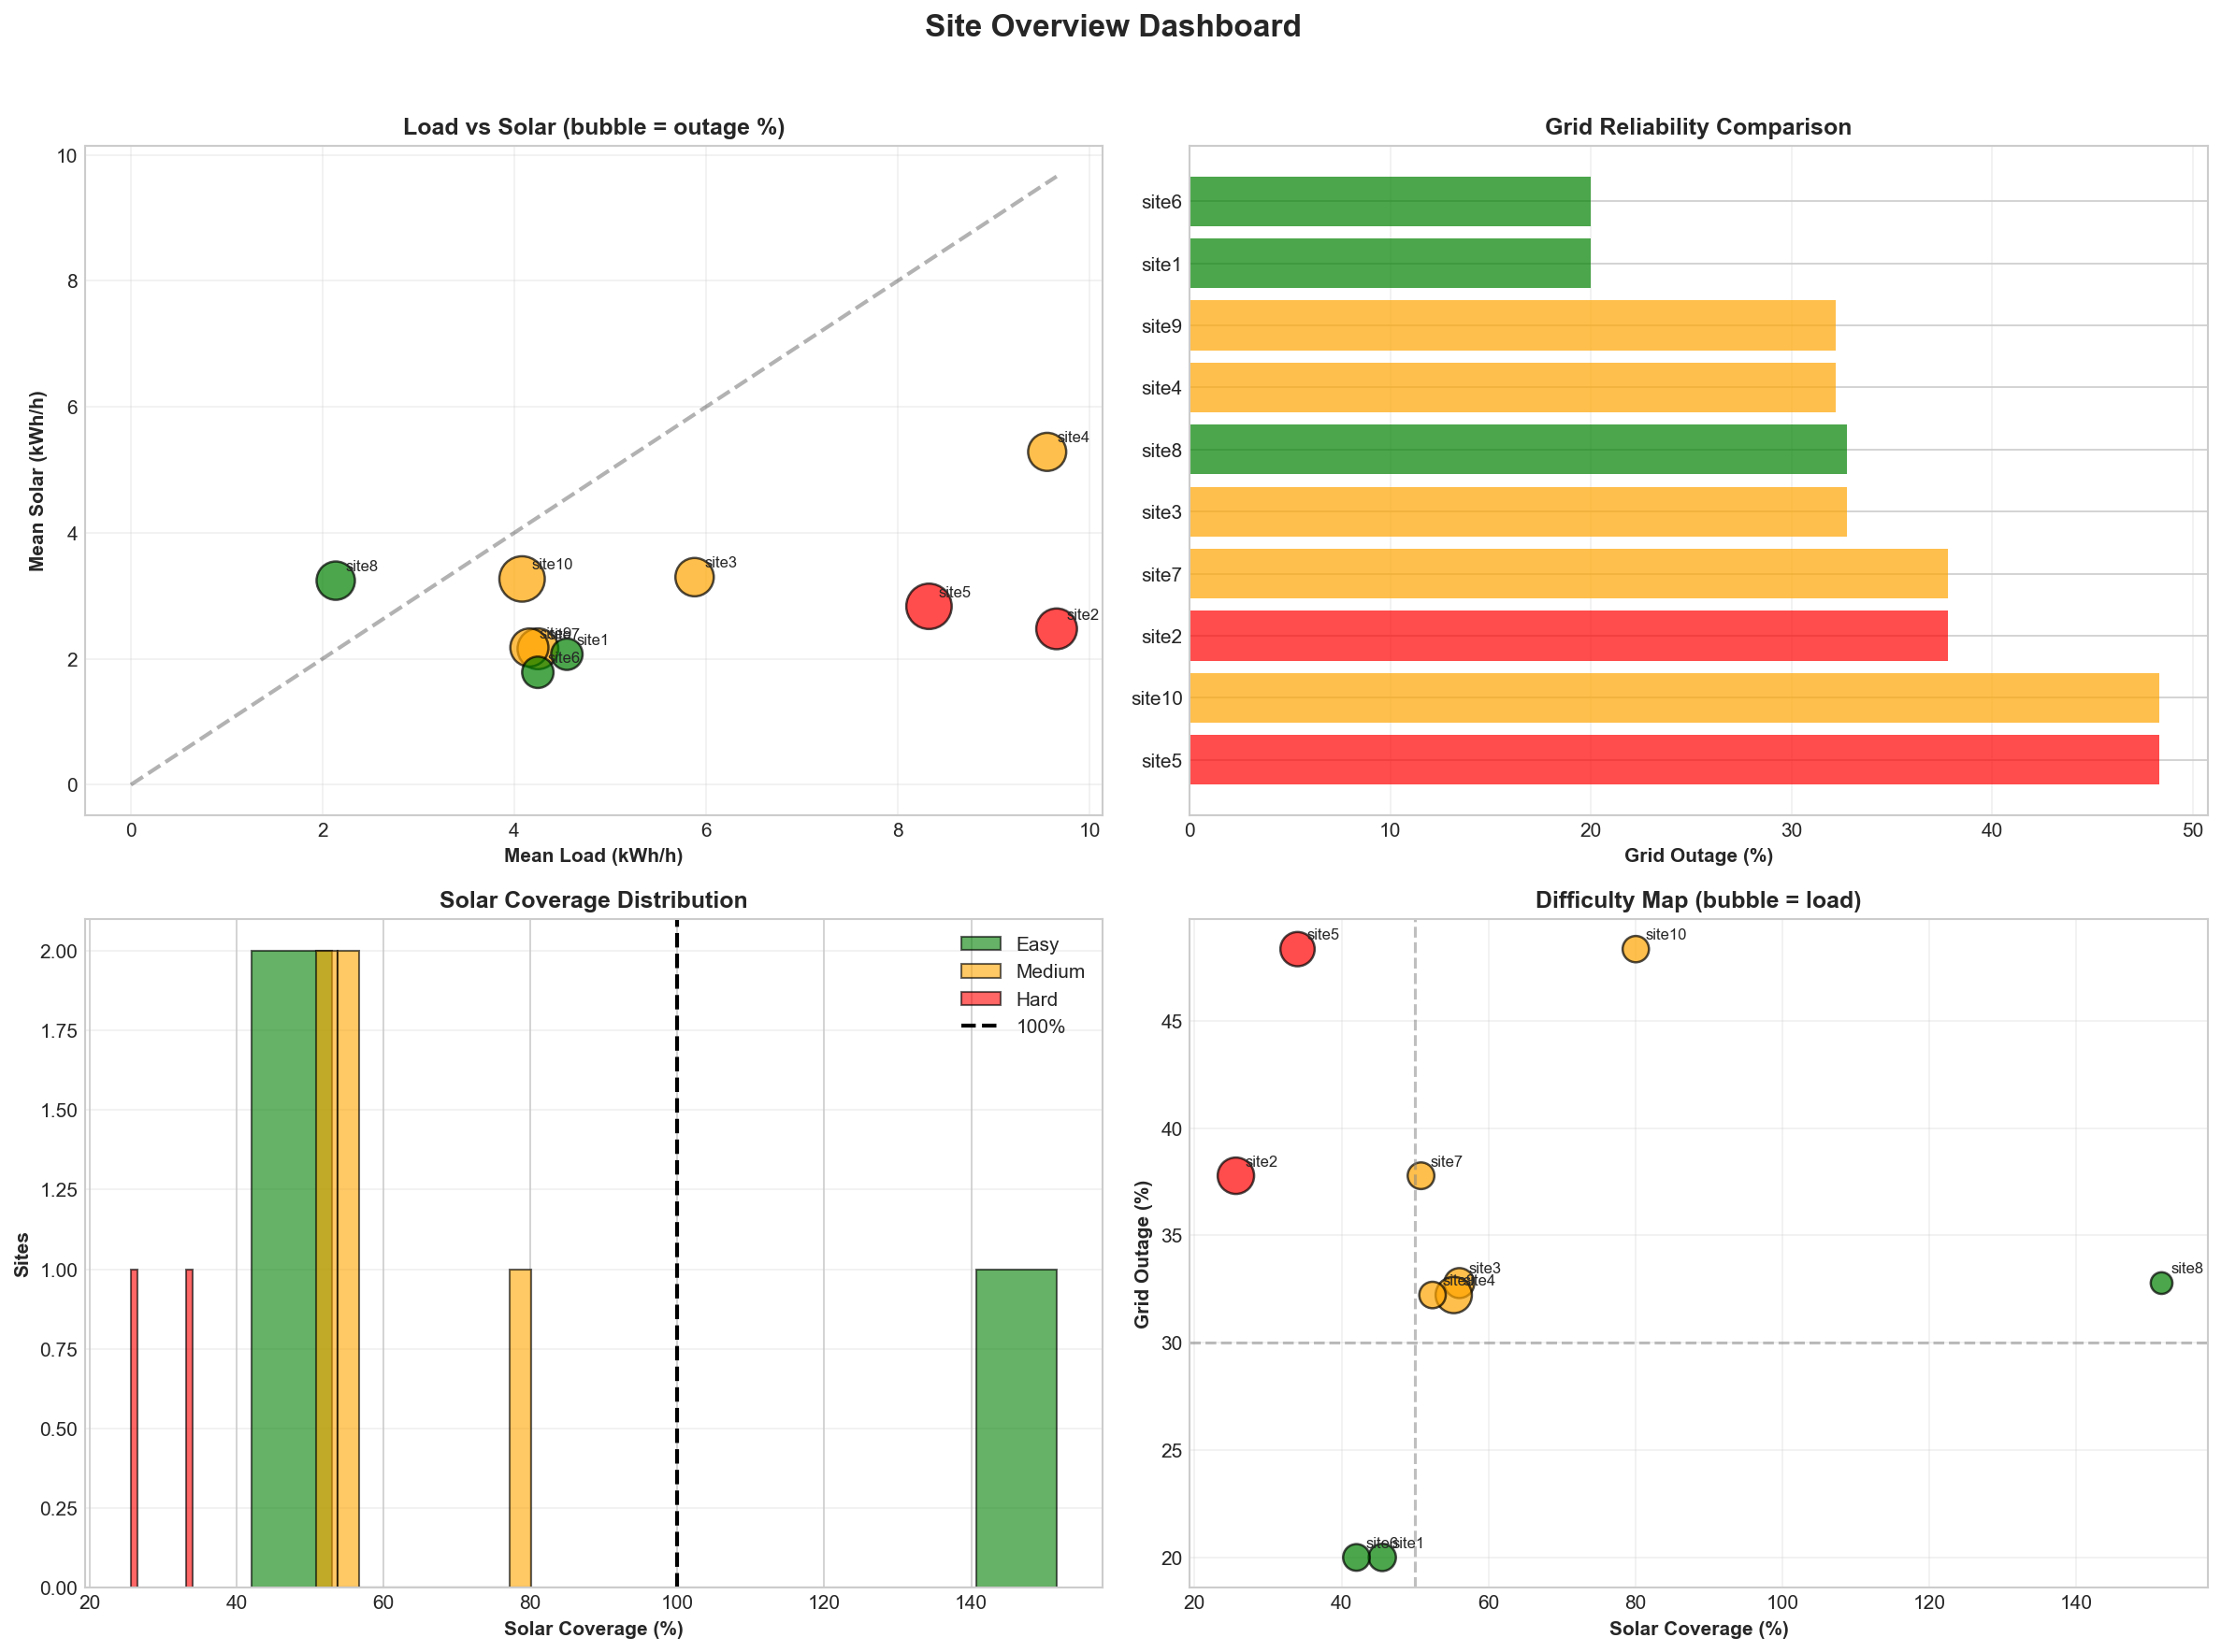
\includegraphics[width=\textwidth, clip=true]{images/fig1_site_overview}
\caption{Site overview dashboard for all ten ITU/Zindi sites.
\textit{Top-left:} mean load vs.\ mean solar scatter; bubble size encodes
outage rate.  Sites above the diagonal are solar-surplus; sites below are
solar-deficit.  \textit{Top-right:} grid outage rate per site, sorted by
severity; sites~5 and~10 have the highest outage exposure ($\approx$48\%).
\textit{Bottom-left:} distribution of solar coverage levels; one site
(site~8) exceeds 100\%.  \textit{Bottom-right:} difficulty map — solar
coverage vs.\ grid outage rate with bubble size proportional to load;
Hard sites (red) occupy the high-outage, low-solar quadrant.}
\label{fig:site_characteristics}
\end{figure}

Three observations emerge from the site statistics.

\textbf{High-load, low-solar, weak-grid sites are the most difficult.}
Sites~2 and~5 combine high average demand (9.66 and 8.32\,kWh/h), poor
solar coverage (25.6\% and 34.0\%), and frequent grid outages (62.2\% and
51.7\% availability).  These sites create persistent energy deficits during
grid loss and place the greatest pressure on diesel backup and fuel inventory
management.

\textbf{Site~8 is solar-surplus.}
With solar coverage of 151.6\%, site~8 generates more PV energy than it
consumes on average.  DG activation is rare; reliability is rarely
threatened.  This site establishes a natural performance ceiling against
which other sites can be compared.

\textbf{Battery capacity is not uniformly matched to load.}
Despite having the highest outage frequency in the dataset, site~5 has only
20.5\,kWh of battery storage --- less than high-load sites~2, 3, and~4 which
carry 41\,kWh banks.  On site~5, diesel inventory is therefore a primary
reliability lever even after battery dispatch is optimised.


% ============================================================
\section{Diurnal Load and Solar Patterns}
\label{sec:diurnal_patterns}
% ============================================================

In addition to cross-site variability, the dataset exhibits a clear and
structured diurnal pattern.  Figure~\ref{fig:diurnal_profiles} shows the mean
hourly load demand and mean hourly solar generation averaged across all sites.

\begin{figure}[htbp]
\centering
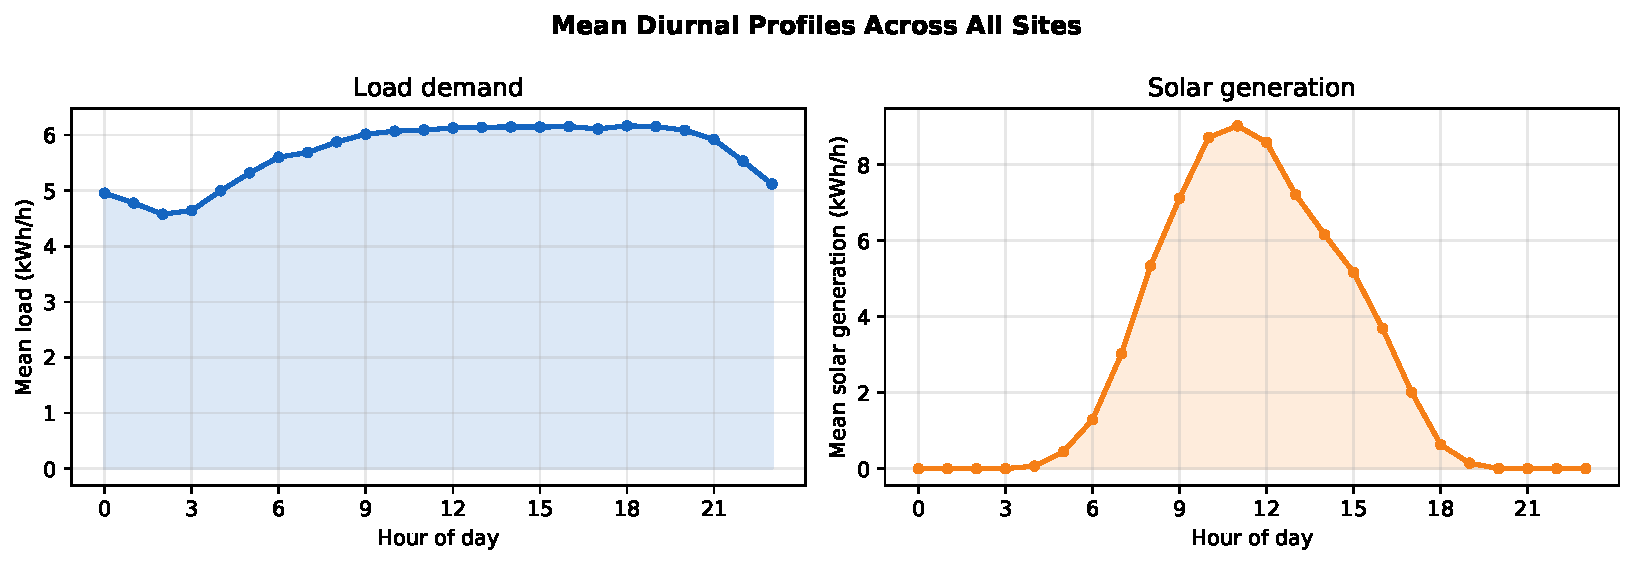
\includegraphics[width=\textwidth, clip=true]{images/fig_diurnal_profiles}
\caption{Mean diurnal load and solar profiles averaged across all ten sites.
Load is elevated from 08:00--20:00, peaking near 6.2\,kWh/h in the
mid-afternoon.  Solar generation peaks near 11:00 at 9.0\,kWh/h before
declining through the afternoon.  The temporal mismatch between peak solar
(11:00) and peak load (14:00--18:00) creates a recurring afternoon deficit
window that battery, grid, or DG must cover.}
\label{fig:diurnal_profiles}
\end{figure}

Two observations are relevant to the control problem.  First, solar generation
is effectively zero from 20:00 to 05:00; all overnight demand must be met by
stored energy, grid supply, or DG operation.  Second, although mean daytime
solar output is substantial, it does not perfectly align with demand: the
solar peak precedes the load peak by several hours.  This creates predictable
deficit windows before sunrise and in the late afternoon, reinforcing the need
for sequential energy management rather than purely myopic dispatch.


% ============================================================
\section{Grid Outage Structure}
\label{sec:grid_patterns}
% ============================================================

Grid availability is a defining feature of the dataset because it is the
primary exogenous disturbance that forces switching between renewables,
battery, and diesel-backed operation.  Figure~\ref{fig:grid_raster} shows the
hour-by-hour outage raster for all ten sites over the full 60-day window.

\begin{figure}[htbp]
\centering
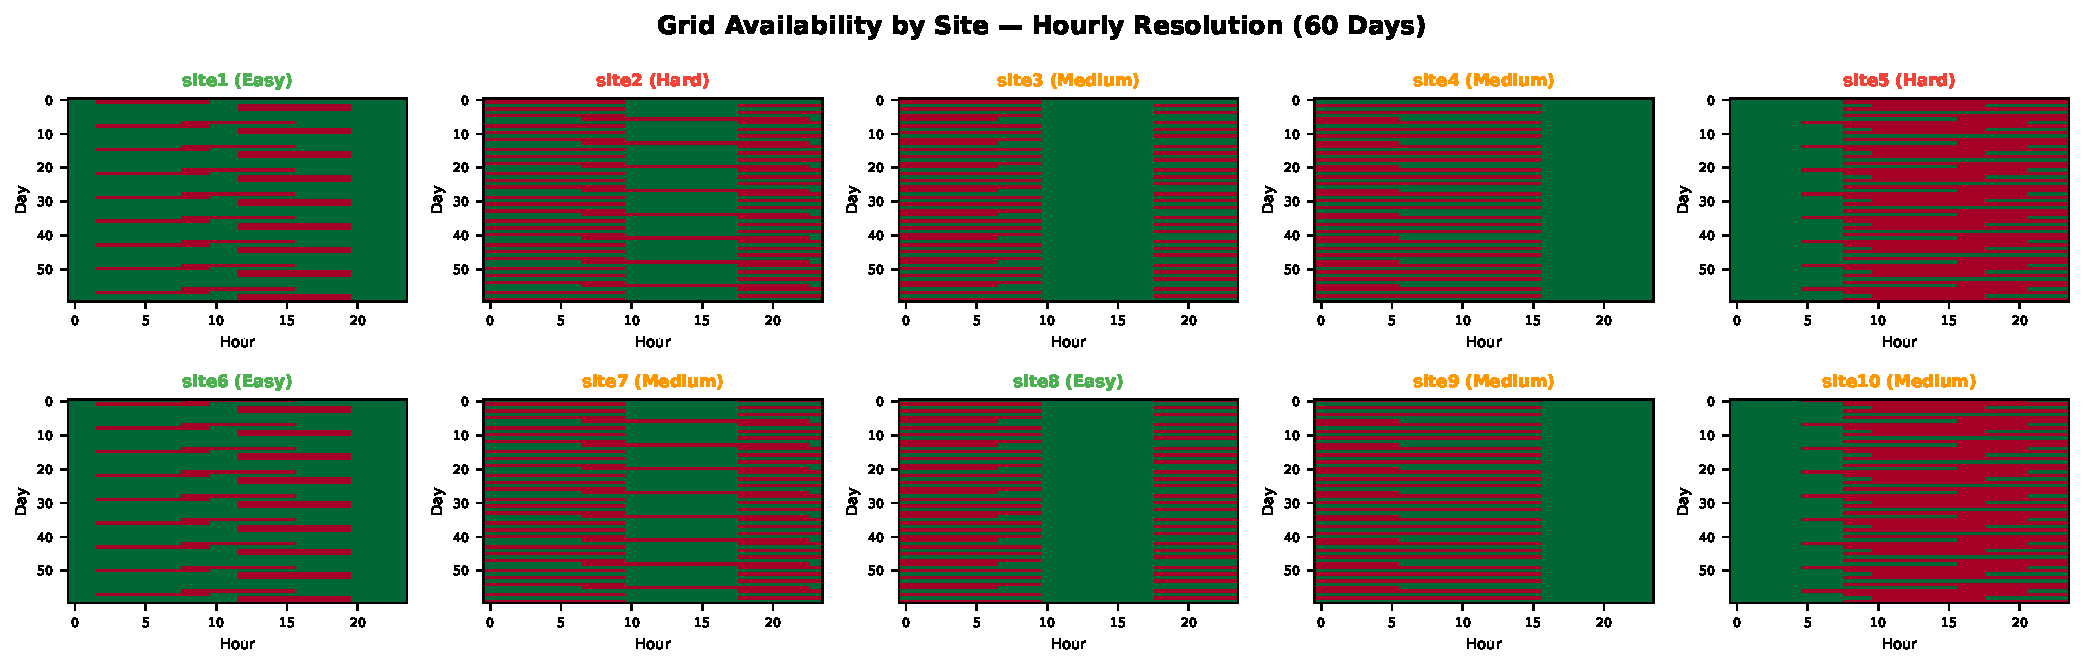
\includegraphics[width=\textwidth, clip=true]{images/fig_grid_raster}
\caption{Grid availability raster: each row is one day, each column one hour
of day.  Green = grid available; red = outage.  Sites~1 and~6 show short,
structured nocturnal outages (8\,h blocks).  Sites~2, 5, 7, and~10 exhibit
extended daily outage patterns (up to 16\,h).  The block structure indicates
that outages are not purely random but follow a predictable daily schedule,
a regularity that a non-myopic RL policy can exploit.}
\label{fig:grid_raster}
\end{figure}

Table~\ref{tab:outage_stats} quantifies outage structure per site.  The
maximum observed outage duration is 16\,h across all sites.  This exceeds the
24-h mean lead time of the normal logistics scenario, confirming that a single
extended outage can deplete a partially-stocked tank before a delivery
arrives --- the core failure mode the inventory-aware policy must prevent.

\begin{table}[htb]
\centering
\small
\caption{Grid outage statistics per site.}
\label{tab:outage_stats}
\begin{tabular}{lrrrl}
\toprule
\textbf{Site} & \textbf{Outage events} & \textbf{Mean duration (h)} &
\textbf{Max duration (h)} & \textbf{Class} \\
\midrule
site1  & 36 &  8.0 &  8 & Easy   \\
site2  & 34 & 16.0 & 16 & Hard   \\
site3  & 34 & 13.9 & 16 & Medium \\
site4  & 34 & 13.6 & 16 & Medium \\
site5  & 52 & 13.4 & 16 & Hard   \\
site6  & 36 &  8.0 &  8 & Easy   \\
site7  & 34 & 16.0 & 16 & Medium \\
site8  & 34 & 13.9 & 16 & Easy   \\
site9  & 34 & 13.6 & 16 & Medium \\
site10 & 52 & 13.4 & 16 & Medium \\
\bottomrule
\end{tabular}
\end{table}

Site~5 stands out with 52 outage events --- the highest frequency in the
dataset --- combined with the lowest solar coverage and a small battery.
This triple constraint makes it the most demanding test for any inventory or
dispatch policy, and it is expected to be among the most informative sites
in the experimental evaluation.


% ============================================================
\section{Scarcity and Surplus Regimes}
\label{sec:scarcity_surplus}
% ============================================================

Exploratory analysis reveals that the dataset naturally separates into two
operational regimes.

\textbf{Scarcity regime.}
In several sites, mean deficit during outage is high and battery autonomy is
insufficient to cover the longest observed outage block.  In such settings,
diesel is not a marginal backup but a critical reliability resource.  A
controller that ignores fuel inventory in these sites risks stockout during
repeated weak-grid periods.  Figure~\ref{fig:rl_stress} quantifies this
across four dimensions: battery autonomy relative to grid outage frequency,
battery sizing against worst-case outage duration, 95th-percentile deficit
severity during outages, and the fraction of solar-surplus hours per site.

\begin{figure}[htbp]
\centering
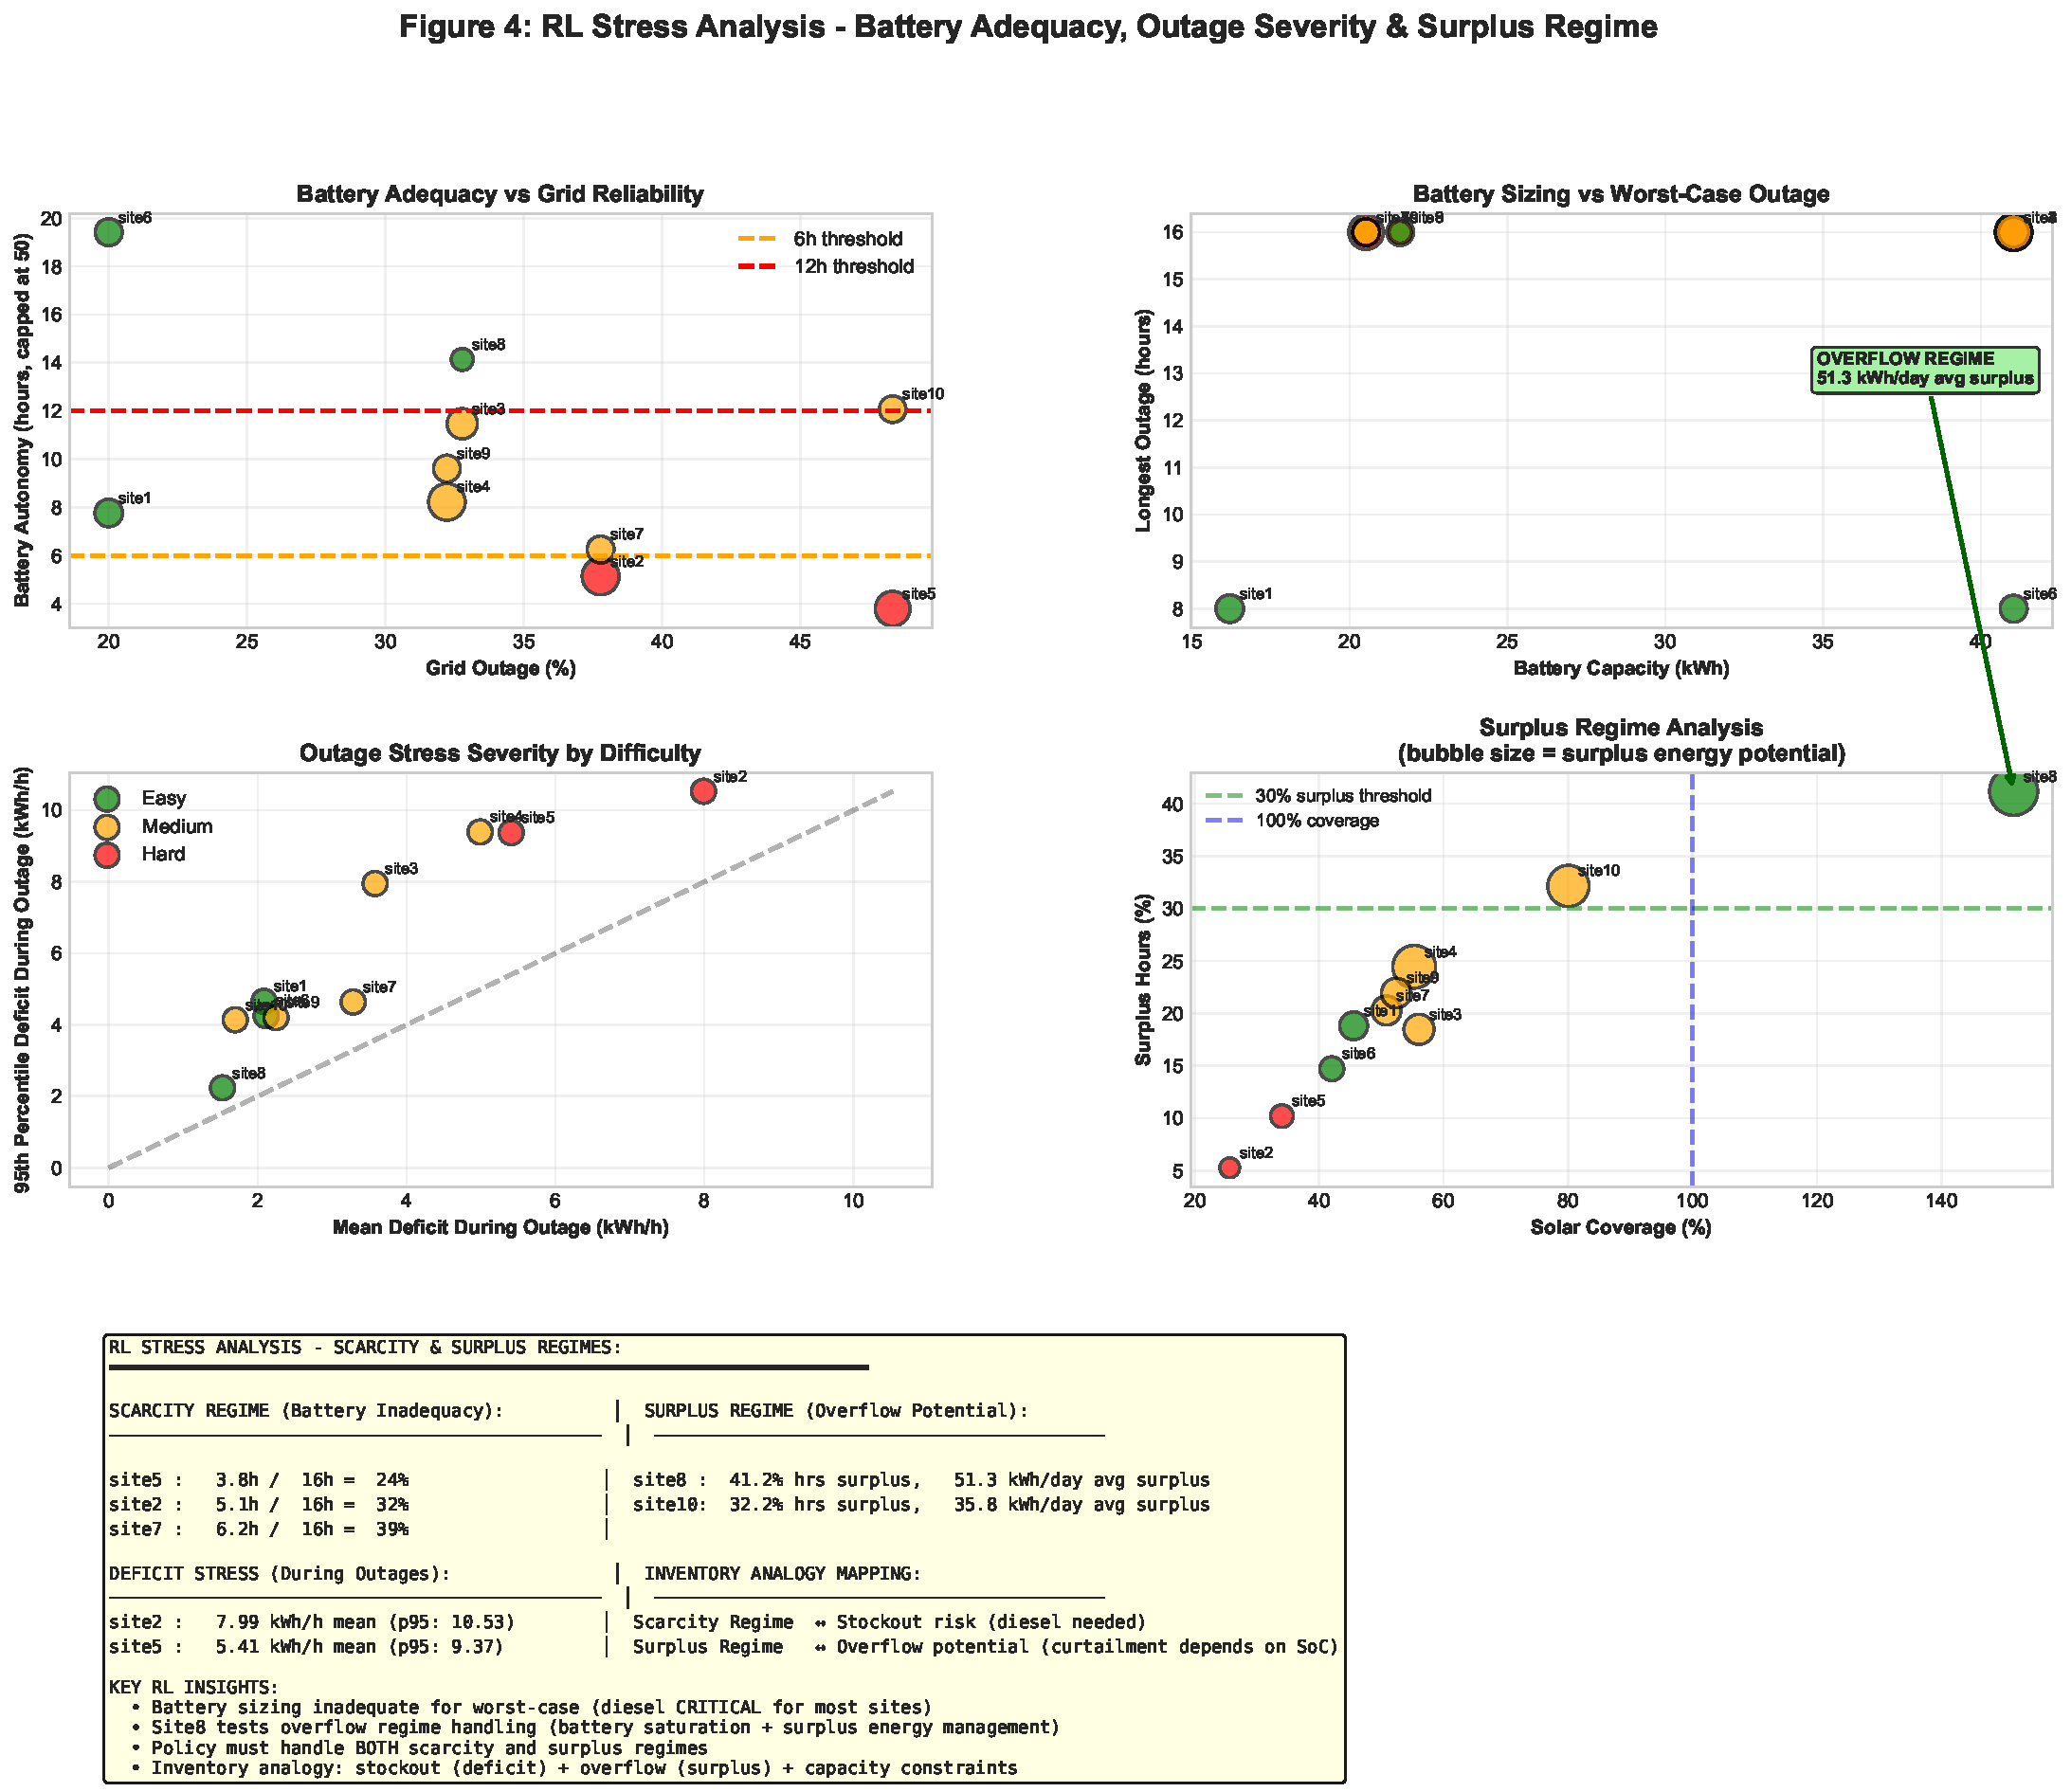
\includegraphics[width=\textwidth, clip=true]{images/fig4_rl_stress_analysis}
\caption{RL stress analysis across all ten sites.
\textit{Top-left:} battery autonomy (hours) vs.\ grid outage rate; sites
below the 6\,h threshold (orange dashed) cannot bridge a typical outage on
battery alone.  Sites~2 and~5 fall well below this line.
\textit{Top-right:} battery capacity vs.\ longest observed outage; most sites
face worst-case outages of 16\,h with batteries sized for far less.
\textit{Bottom-left:} mean vs.\ 95th-percentile deficit during outages;
sites~2 and~5 (red) show the highest deficit stress.
\textit{Bottom-right:} surplus hours vs.\ solar coverage; site~8 is in the
overflow regime with 41\% surplus hours and 51\,kWh/day average surplus.
The summary panel confirms the scarcity--surplus split: sites~2 and~5 are
battery-inadequate (inventory-critical), while site~8 and partially site~10
face overflow potential.}
\label{fig:rl_stress}
\end{figure}

Figure~\ref{fig:net_load_cdf} shows the net load
CDF for all sites; the Hard sites (site~2 and site~5, red) have right-shifted
distributions, confirming sustained positive net load and high reliance on
supplementary energy sources.

\textbf{Surplus regime.}
At the other extreme, site~8 is clearly solar-surplus, with solar coverage
of 151.6\% and net load negative for 41\% of hours (average surplus
51\,kWh/day).  Solar generation peaks at 10.5\,kWh/h near 10:00 while
load holds steady near 2\,kWh/h, saturating the 21.6\,kWh battery on
most days.  Here the main challenge is not avoiding shortage but handling
battery saturation and curtailment.  Site~8 behaves qualitatively
differently from the scarcity-dominated sites; its detailed profile is
in Appendix~\ref{app:site_profiles}.

\begin{figure}[htbp]
\centering
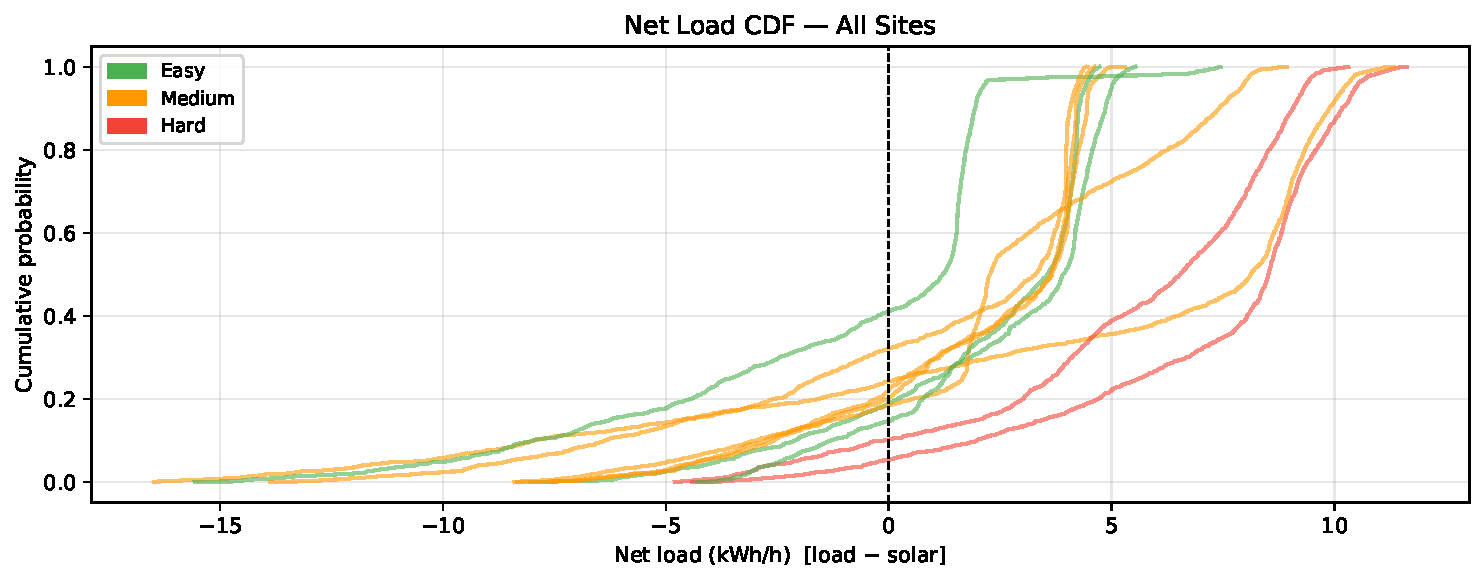
\includegraphics[width=0.85\textwidth, clip=true]{images/fig_net_load_cdf}
\caption{Cumulative distribution of net load across all sites.  The dashed
vertical line at zero separates solar-deficit hours (right) from solar-surplus
hours (left).  Hard sites (red) are entirely in deficit; site~8 (green) crosses
zero near $p = 0.6$, confirming majority solar surplus.}
\label{fig:net_load_cdf}
\end{figure}

This regime split is important for the experimental design.  Easy and
surplus-regime sites are useful robustness checks but offer limited
discriminatory power where operating conditions are mild.
The scarcity-regime sites --- primarily site~2, site~5, and site~10 under
adverse logistics conditions --- are structurally where inventory-aware
control is most likely to reveal a measurable advantage.

\begin{quote}
\textbf{Note on site terminology used elsewhere in this thesis.} This
scarcity-regime grouping (site~2, site~5, site~10) and the Hard/Medium/Easy
difficulty classification of Section~\ref{sec:site_classification} below
are both derived from the EDA in this chapter. A separate, differently
selected three-site subset (site~2, site~5, site~7) is used in
Chapter~\ref{chap:results} for finer-grained sensitivity analyses; that
subset was chosen to provide diverse operating characteristics (load,
solar generation and outage behaviour) for the detailed sensitivity
analyses, rather than to represent the scarcity-based difficulty ranking
introduced in this chapter. The scarcity-regime classification introduced
here is therefore used for exploratory data analysis, whereas the
site~2/site~5/site~7 subset supports the controlled experimental
comparisons described in Chapters~\ref{chap:methodology}
and~\ref{chap:results}.
\end{quote}


% ============================================================
\section{Representative Site Profile}
\label{sec:site_profiles}
% ============================================================

To make the stress analysis concrete, Figure~\ref{fig:site5_analysis}
presents the enhanced profile for site~5 --- the most operationally
demanding site in the dataset and the primary test case for
inventory-aware control.  Profiles for all ten sites are provided in
Appendix~\ref{app:site_profiles}.

Site~5 combines high outage frequency (52 events over 60 days, the
highest in the dataset), low solar coverage (34\%), and a small battery
(20.5\,kWh, autonomy 3.8\,h).  The battery covers only 24\% of the
longest observed 16-hour outage.  Four outage events exceed the 12-hour
threshold.  Outage-conditioned mean deficit is 5.41\,kWh/h (95th
percentile 9.37\,kWh/h).  Under these conditions any policy that
underestimates diesel consumption risk faces repeated unserved load
events.
 This site therefore provides one of the most discriminating test
cases for comparing inventory-aware and inventory-blind control.

\begin{figure}[htbp]
\centering
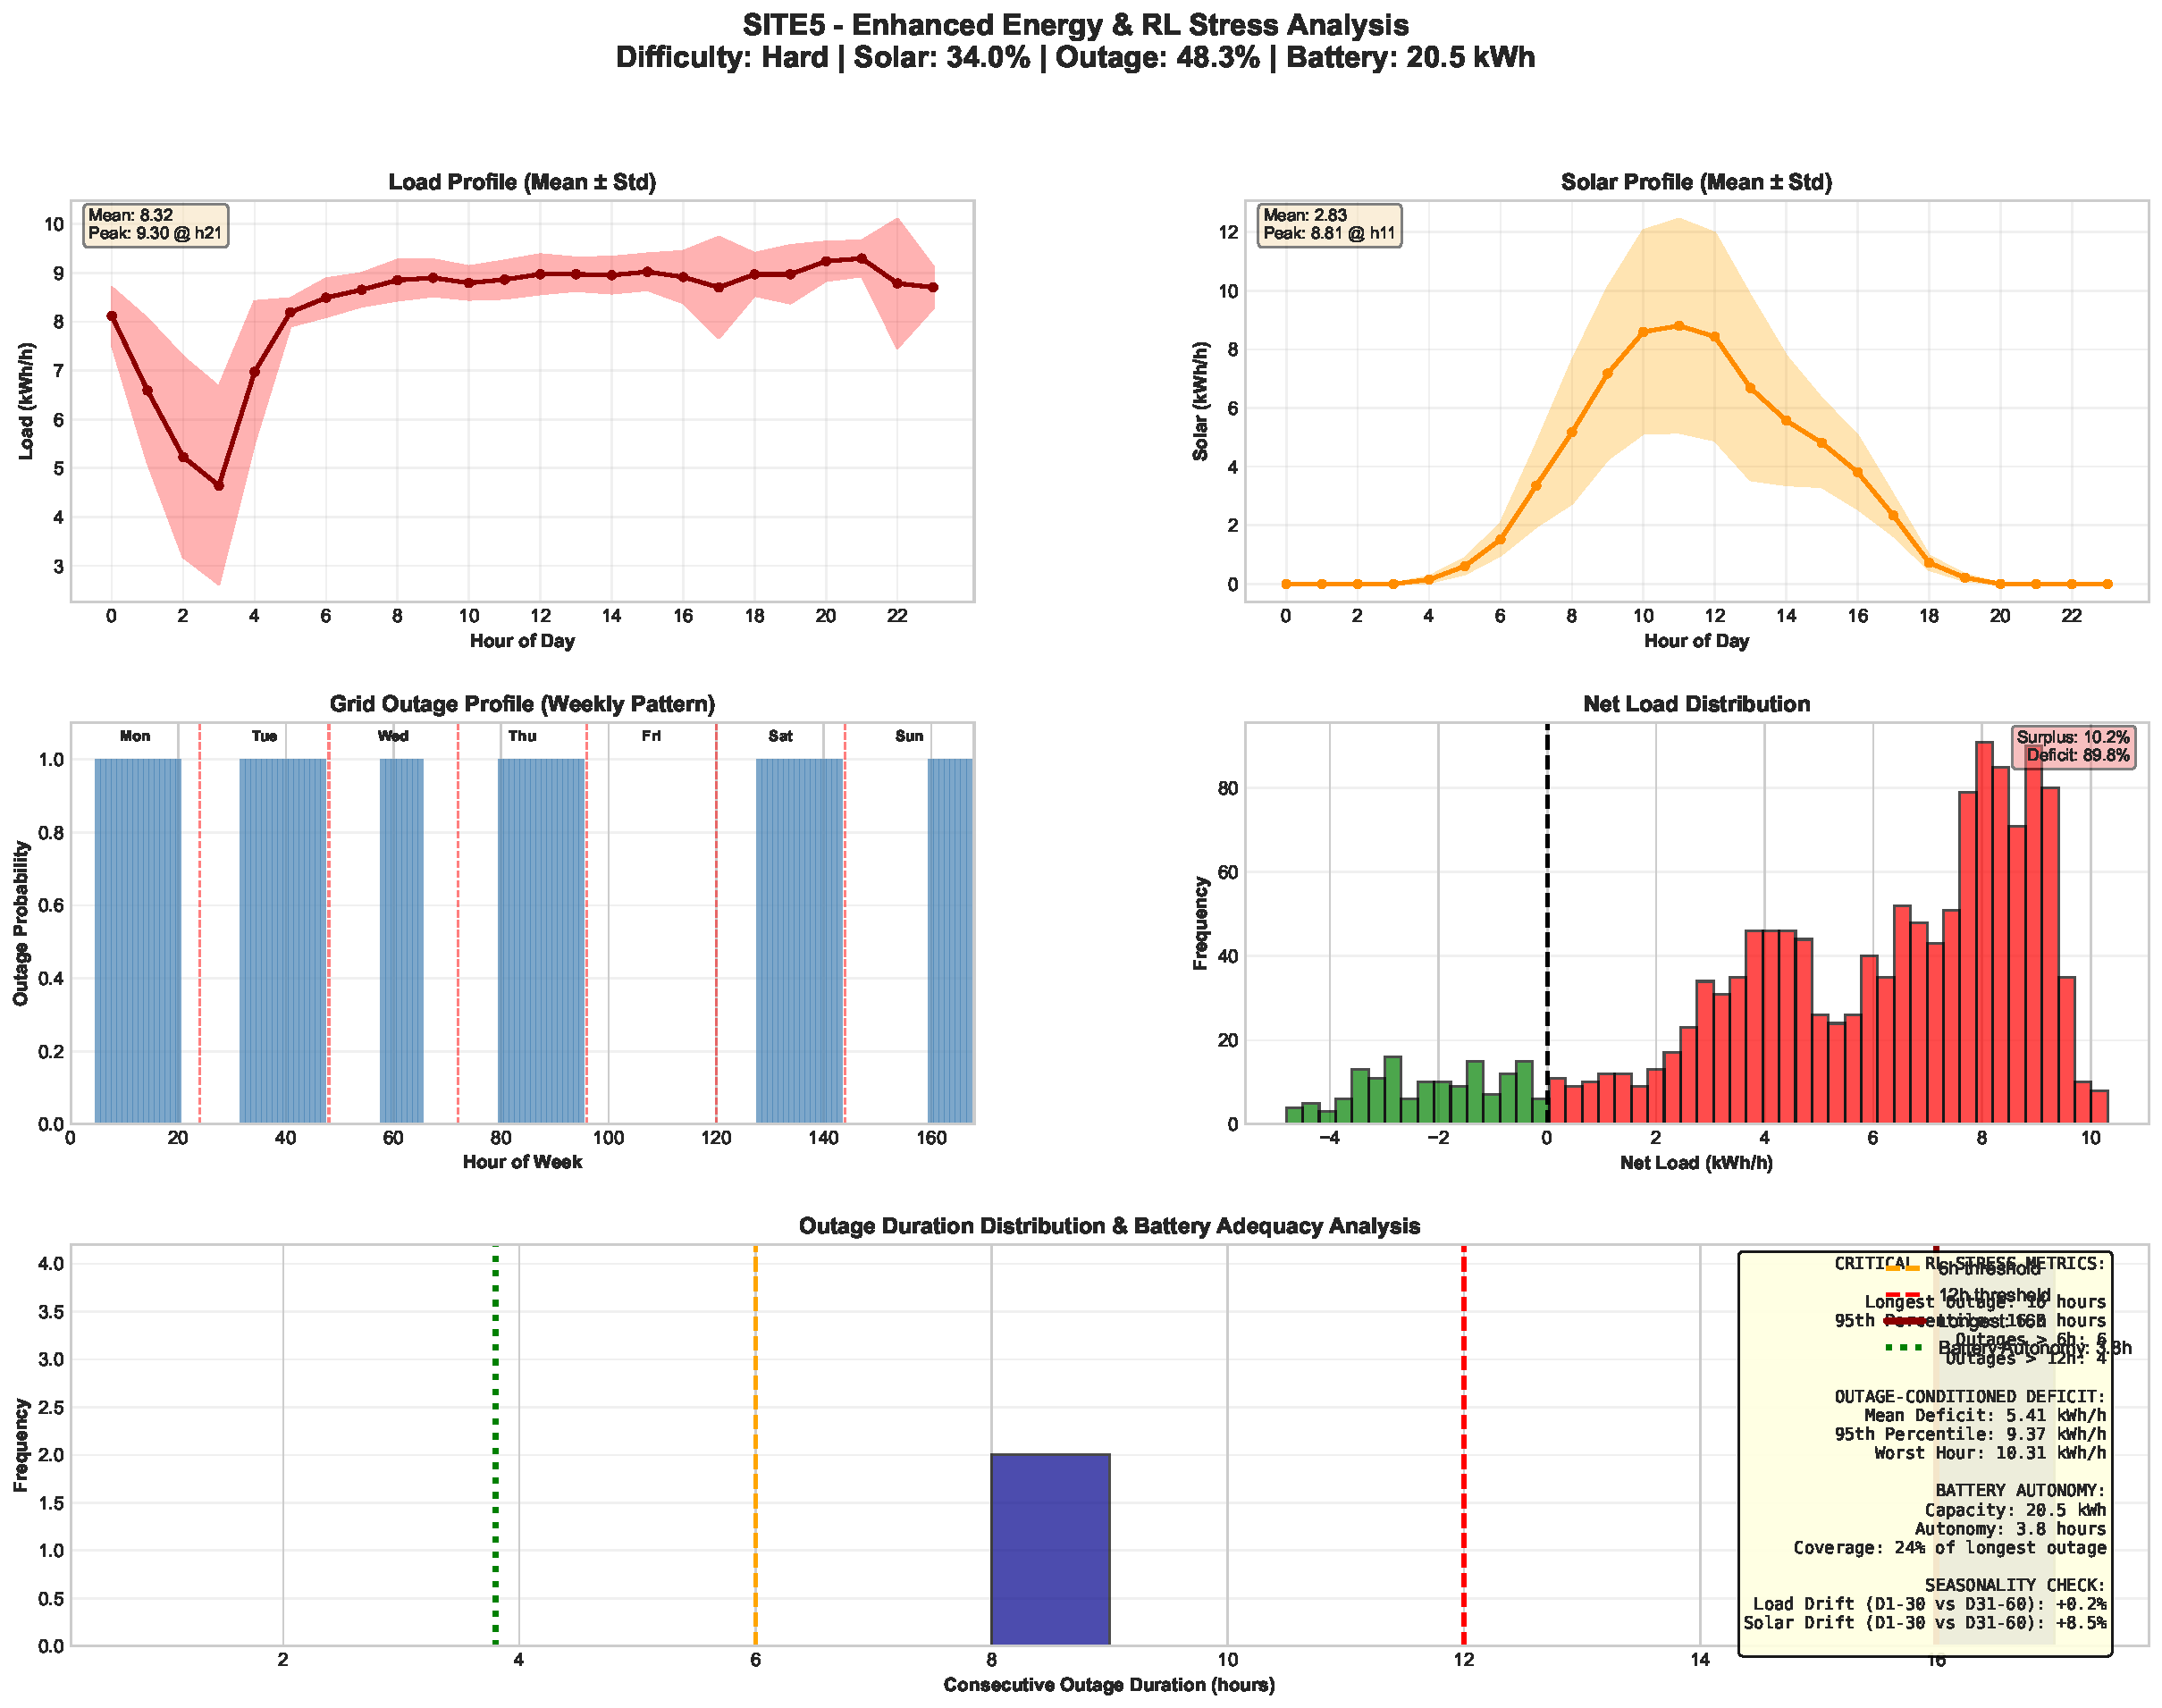
\includegraphics[width=\textwidth, clip=true]{images/site5_enhanced_analysis}
\caption{Enhanced stress analysis for site~5 (Hard).
Battery autonomy of 3.8\,h covers only 24\% of the longest outage.
52 outage events over 60 days --- the highest frequency in the dataset.
Four events exceed the 12-hour threshold (red dashed line).
Outage-conditioned 95th-percentile deficit is 9.37\,kWh/h.}
\label{fig:site5_analysis}
\end{figure}


% ============================================================
\section{Site Difficulty Classification}
\label{sec:site_classification}
% ============================================================

To organise the experiments, sites are grouped into difficulty classes using a
composite score combining grid outage frequency, solar coverage, and mean net
load.  Sites scoring 4 are classified Hard; 2 Medium; 1 Easy.
Table~\ref{tab:difficulty} shows the classification.

\begin{table}[htb]
\centering
\small
\caption{Site difficulty classification and primary challenge.  Constrained
sites (frequent outages, low solar, inadequate battery autonomy) receive
focused statistical analysis in Chapter~\ref{chap:results}.}
\label{tab:difficulty}
\begin{tabular}{p{3.8cm}p{1.5cm}p{1.5cm}p{5.0cm}}
\toprule
\textbf{Site(s)} & \textbf{Class} & \textbf{Outage (\%)} & \textbf{Primary challenge} \\
\midrule
site2, site5                       & Hard   & 38--48 & High load, low solar, frequent outages;
                                                        battery autonomy inadequate for longest outages \\
site3, site4, site7, site9, site10 & Medium & 33--48 & Moderate load-solar balance; grid
                                                        reliability moderate \\
site1, site6, site8                & Easy   & 20--33 & Adequate solar or high grid availability;
                                                        outage stress low \\
\bottomrule
\end{tabular}
\end{table}

\begin{quote}
\textbf{Note on site~10.}
Site~10 is classified Medium by composite score (solar coverage 80\%, but
outage frequency 51.7\%).  Its battery autonomy of 12.1\,h covers only
75\% of the longest observed 16-hour outage, and four outage events exceed
the 12-hour threshold.  Under adverse logistics conditions, site~10 is
structurally exposed to the same reliability risks as the Hard sites.
Results tables note this distinction where relevant.
\end{quote}

The classification is a practical organising tool, not a research outcome.
It separates sites where operating stress is structurally high
from those where conditions are comparatively mild.


% ============================================================
\section{Dataset Limitations}
\label{sec:dataset_limitations}
% ============================================================

The dataset is well suited to the present study, but three limitations must
be stated clearly.

\textbf{No diesel logistics records.}
The dataset provides load, solar, grid availability, and battery capacity, but
not diesel delivery events, lead times, or fuel replenishment logs.  The
delivery-pipeline component of the simulator is therefore synthetic.  This
is the sole component of the simulation not grounded in the ITU data, and
is clearly documented as such in Chapter~\ref{chap:methodology}.

\textbf{Limited time horizon.}
Each site contains 60 days of observations, covering a single operating
season.  Solar generation patterns and outage frequencies may differ in other
seasons; results should be interpreted as representative of the recorded
conditions rather than year-round operation.

\textbf{Assumed tank capacity.}
Absolute diesel tank capacity is not provided.  The assumption
$C^{\Tank} = 72\bar{D}$ gives physically plausible values (approximately
three days of full-load backup across all sites), but real tank sizes may
differ.  Sensitivity to this assumption is partially captured by randomising
initial inventory over $[0.3,\,0.9]\,C^{\Tank}$ during evaluation.


% ============================================================
\section{Chapter Summary}
\label{sec:dataset_summary}
% ============================================================

This chapter established the empirical foundation of the study.  The
ITU/Zindi dataset provides ten heterogeneous tower sites with hourly load,
solar, and grid traces that are replayed directly in the simulator.
Preprocessing produces clean site-level time series with consistent indexing,
derived net load, and a principled train/test split.  Exploratory analysis
shows that the sites span both scarcity-dominated and surplus-dominated
regimes, with large differences in outage severity, battery adequacy, and
renewable coverage.  These characteristics justify the multi-site evaluation
design used in the remainder of the thesis and explain why inventory-aware
control is most likely to show a measurable advantage in the most constrained
sites.
    % filename: chap-experimental-execution-FIXED.tex
\chapter{Experimental Execution and Implementation}
\label{chap:experimental-execution}
\setlength{\emergencystretch}{1.5em}   % prevents right-margin overflow in this chapter

Chapter~\ref{chap:methodology} defined the experimental design: the
simulator architecture, policy set, and evaluation protocol.  The present
chapter documents how that design was executed in practice.  It records the
engineering decisions made during implementation, summarises the training
workload carried out across all sites and seeds, and explains how the final
ablation set evolved from the original experimental plan.  The objective is
to provide transparency on the experimental execution while avoiding
duplication of the methodological definitions already presented in
Chapter~\ref{chap:methodology}.


% ============================================================
\section{Implementation Overview}
\label{sec:impl_overview}
% ============================================================

The implementation was built in layers, each producing runnable and testable
output before the next layer began.  This strategy ensured that no layer
depended on untested components from a lower layer, and that partial results
were available at every stage.

\begin{table}[htb]
\centering
\small
\caption{Implementation execution sequence.}
\label{tab:impl_sequence}
\begin{tabular}{lll}
\toprule
\textbf{Layer} & \textbf{Component} & \textbf{Deliverable} \\
\midrule
1 & Data pipeline   & ITU/Zindi site CSVs loaded, validated, split \\
2 & Simulator       & \texttt{TelecomEnv} passing unit tests on all transitions \\
3 & Baselines       & B0, B1 rule-based policies producing first cost numbers \\
4 & RL agent        & RLInv training on single site converging \\
5 & Track B         & Hierarchical $(s,S)$ + PPO dispatch training \\
6 & Ablations       & A5, A6, A7 variants trained and evaluated \\
7 & Evaluation      & Full 1{,}800-rollout evaluation campaign complete \\
\bottomrule
\end{tabular}
\end{table}

The data pipeline and simulator (layers~1--2) were implemented and validated
before any policy training began.  Because all policies share the same
environment, correctness of the simulator was verified first to avoid
propagating modelling errors into downstream policy comparisons.
Rule-based baselines (layer~3) were implemented next because they require
no training and immediately produce interpretable cost numbers that serve as
sanity checks for the environment dynamics.

% FIX page 95: split the long path-string sentence across lines using \allowbreak
The repository structure follows the layer ordering:
\texttt{env/},
\texttt{baselines/},
\texttt{models/},
\texttt{train/},
\texttt{eval/},
with all hyperparameters in a single
\texttt{config/\allowbreak hparams.yaml}
and no magic numbers in training scripts.


% ============================================================
\section{Simulator Implementation Decisions}
\label{sec:impl_decisions}
% ============================================================

Several design decisions were made during simulator implementation that
diverge from or refine the formal model of Chapter~\ref{chap:problem}.
Each decision was made for a specific practical reason and is documented
here for reproducibility and examiner transparency.

\paragraph{Geometric rather than lognormal lead-time model.}
The formal model specified a lognormal lead-time distribution.  During
implementation, the geometric distribution was adopted instead.  The
geometric model preserves the Markov property: the probability of delivery
at each step is constant regardless of how long the order has been in
transit.  This means the pending-order state can be represented as a
two-scalar tuple (flag, quantity) rather than a countdown vector, keeping
the observation space low-dimensional.  The mean lead times are matched
between the two parameterisations (24\,h normal, 48\,h delayed), so the
operational stress is equivalent.

\paragraph{Discrete order actions.}
The formal model allowed a continuous order quantity.  The implementation
uses three discrete order levels: zero, $0.30\,C^{\Tank}$, and
$0.60\,C^{\Tank}$.  Discrete actions simplify the policy gradient
computation and match the physical reality of tanker deliveries, which
arrive in fixed load sizes rather than arbitrary quantities.  The reduction
from continuous to discrete was confirmed not to restrict meaningful
ordering behaviour: all three levels are exercised by the trained policies.

% FIX page 96: \allowbreak inside long monospace tokens prevents right-margin overflow
\paragraph{Action masking implementation.}
\texttt{Maskable\-PPO} from \texttt{sb3\-contrib} was used rather than
implementing a custom masking layer.  The library applies the mask by
setting infeasible action logits to $-\infty$ before the softmax, making
the probability of any infeasible action exactly zero by construction.
This required integrating a mask-computation function into the
environment's \texttt{step()} call and passing it through the
\texttt{Subproc\-Vec\-Env} wrapper --- a non-trivial integration verified
by checking that no illegal actions appeared in 10{,}000 random rollouts.

\paragraph{Tank capacity derivation.}
The ITU dataset does not provide absolute diesel tank capacity.  Tank
capacity was set to $C^{\Tank} = 72\,\bar{D}$ kWh-equivalent, where
$\bar{D}$ is the site mean hourly load, giving approximately three days
of full-load backup.  This convention was applied consistently across all
ten sites and produces physically plausible values.

\paragraph{Observation normalisation synchronisation.}
\texttt{Vec\-Normalize} accumulates running mean and variance statistics
during training.  If these statistics are not explicitly frozen and
synchronised before evaluation, the normalisation applied to evaluation
observations differs from that seen during training, causing a systematic
input-scale mismatch.  A custom evaluation callback was implemented to
copy the training \texttt{Vec\-Normalize} state to the evaluation
environment before each validation pass.  Without this fix, early
evaluation results showed anomalously high variance across seeds that
disappeared once the synchronisation was corrected.
\sloppy
\paragraph{Parallel environment count.}
The training configuration targeted eight parallel workers using
\texttt{Subproc\-Vec\-Env}, following the architecture plan.  On
the Windows development machine, the OS process-handle limit caused
intermittent failures at eight workers.  The parallel environment count
was reduced to four workers for all training runs.  This doubles
wall-clock training time per run but does not affect the statistical
properties of the PPO gradient estimates, as the effective batch size is
preserved by proportionally increasing $n_{\text{steps}}$.
\fussy
% ============================================================
\section{Training Execution}
\label{sec:training_execution}
% ============================================================

\subsection{Workload summary}

Table~\ref{tab:training_workload} summarises the complete training
workload executed across all policies, sites, and seeds.

% FIX page 97: \small + narrower Note column prevents table overflow
\begin{table}[htb]
\centering
\small
\setlength{\tabcolsep}{5pt}
\caption{Total training workload.}
\label{tab:training_workload}
\begin{tabular}{lrp{5.5cm}}
\toprule
\textbf{Item} & \textbf{Count} & \textbf{Note} \\
\midrule
Sites                    & 10  & All ITU/Zindi sites \\
Seeds per policy         & 3   & Seeds 42, 123, 777 \\
RL policies trained      & 4   & RLInv, TrackB, A5, A6 \\
Non-RL policies          & 3   & B0, B1 (no training); A7 (PPO, no masking) \\
Timesteps per RL run     & 400{,}000 & Per site per seed \\
Total RL training runs   & 120 & 4 policies $\times$ 10 sites $\times$ 3 seeds \\
A7 targeted rerun        & 6   & Sites 5, 10 $\times$ 3 seeds \\
Total training runs      & 126 & Including A7 rerun \\
Approx.\ wall-clock time & $\approx$\,2\,h & Per run, 4-core CPU \\
\bottomrule
\end{tabular}
\end{table}

\subsection{Convergence check}

A convergence check was conducted on three representative sites (1, 5,
and~7) using seed~42, extending training to 560{,}000 steps.  Sites~1
and~7 showed no change in evaluation reward beyond 400{,}000 steps.
Site~5 exhibited high reward variance across independent runs regardless
of training length, consistent with its classification as a
grid-constrained site where episode outcomes are sensitive to the
stochastic lead-time draws.  The 400{,}000-step checkpoint was retained
for all sites and all policies.  Extended training was not pursued
further because the variance on site~5 was attributed to environment
stochasticity rather than insufficient policy training.

\subsection{Training stability}

RLInv and TrackB training was stable across all sites and seeds.  A5
(no inventory observation) showed higher early-episode variance on Hard
sites, consistent with the expectation that removing inventory
information degrades ordering decisions.  A7 (no action masking)
produced unstable training curves on sites~5 and~10, with occasional
reward spikes followed by policy collapse.  For consistency, the final
model checkpoint (rather than a best-episode checkpoint) was used for
all policies.


% ============================================================
\section{Ablation Set Evolution}
\label{sec:ablation_evolution}
% ============================================================

The original experimental plan specified eight ablations labelled A1--A8
following the architecture plan of Section~2 of the project
specification.  The final executed ablation set differs from this plan.
Table~\ref{tab:ablation_evolution} documents every change and the reason
for it.

\begin{table}[htb]
\centering
\small
\caption{Evolution from planned ablation set (A1--A8) to executed set.}
\label{tab:ablation_evolution}
\begin{tabular}{llp{7.0cm}}
\toprule
\textbf{Original label} & \textbf{Final label} & \textbf{Decision and reason} \\
\midrule
A1 (Full SC-PPO)  & RLInv   & Renamed to reflect actual implementation
                               (MaskablePPO flat MLP, not modular SC-PPO) \\
A8 (Hierarchical) & TrackB  & Renamed; calibrated $(s,S)$ + PPO dispatch \\
A5 (No Inv state) & A5      & Retained unchanged \\
A7 (Vanilla PPO)  & A7      & Retained; evaluated on constrained sites only
                               (sites~5 and~10) where masking effect is measurable \\
B0, B1            & B0, B1  & Rule-based baselines added (not in original A1--A8
                               plan); essential anchors for cost comparison \\
\midrule
A2 (No masking alone) & Dropped & A7 already tests the no-masking condition;
                                  A2 was redundant given MaskablePPO design \\
A3 (No Lagrangian)    & Dropped & Lagrangian update was not implemented in the
                                  final system (masking alone drove violations
                                  to zero); A3 has no executable meaning \\
A4 (No recovery)      & Dropped & Recovery policy was not implemented
                                  (masking handles the cases it was designed
                                  for); A4 has no executable meaning \\
A6 (Fixed ordering)   & A6 added & Not in original plan; introduced after
                                   the TrackB comparison was found to be
                                   potentially confounded, providing a
                                   cleaner H1 test by holding dispatch
                                   architecture constant \\
\midrule
\textbf{Final set} & \multicolumn{2}{l}{B0, B1, A5, A6, A7, TrackB, RLInv} \\
\bottomrule
\end{tabular}
\end{table}

The most important change is the addition of A6.  When TrackB results
became available, the comparison between RLInv and TrackB was potentially
confounded because TrackB uses a different dispatch action space in
addition to a different ordering mechanism.  A6 was therefore introduced
to isolate the ordering contribution specifically by holding the dispatch
architecture constant while varying only the ordering mechanism.


% ============================================================
\section{Evaluation Execution}
\label{sec:eval_execution}
% ============================================================

\subsection{Evaluation rollout count}

The evaluation campaign comprised the following rollout workload:

\[
30 \text{ episodes} \times 10 \text{ sites} \times 3 \text{ seeds}
\times 2 \text{ scenarios} = 1{,}800 \text{ rollouts for RLInv and TrackB}
\]

Baselines and ablations were evaluated under the normal scenario only,
giving an additional $30 \times 10 \times 3 = 900$ rollouts per policy.
The total evaluation dataset contains 11{,}160 episode records across all
policies, sites, seeds, and scenarios.

\subsection{Initial inventory randomisation}

Training episodes initialised inventory at a fixed $0.6\,C^{\Tank}$ to
reduce early-episode variance and allow the policy to observe a range of
ordering decisions before inventory reaches critical levels.  Evaluation
episodes randomise initial inventory uniformly over
$[0.3,\,0.9]\,C^{\Tank}$, testing the policy across a realistic range
of starting conditions.  This asymmetry between training and evaluation
initial conditions is a deliberate design choice: a policy that trains
only at $0.6\,C^{\Tank}$ must generalise to lower and higher starting
inventories at evaluation time, which is the realistic deployment
scenario.

\subsection{Evaluation on constrained sites}

The A7 ablation (vanilla PPO without masking) was evaluated only on
sites~5 and~10, the most reliability-constrained sites in the dataset.
Initial trials on less constrained sites did not expose the effect of
removing action masking, because battery autonomy and outage severity
were not sufficient to force frequent infeasible-action situations.
Sites~5 and~10 were therefore selected for the targeted rerun because
their battery autonomy (3.8\,h and 12.1\,h respectively) and outage
frequency (48.3\% both) make constraint violations much more likely
without masking.


% ============================================================
\section{Metrics and Statistical Framework}
\label{sec:metrics}
% ============================================================

\subsection{Operational metrics}

Table~\ref{tab:metrics} defines the primary metrics computed from each
evaluation episode.

\begin{table}[htb]
\centering
\small
\caption{Evaluation metrics and their operational interpretation.}
\label{tab:metrics}
\begin{tabular}{lp{4.2cm}p{4.8cm}}
\toprule
\textbf{Metric} & \textbf{Definition} & \textbf{Interpretation} \\
\midrule
EENS (kWh)      & Expected Energy Not Served per episode: $\sum_t U_t$
                & Primary reliability metric.  Zero means
                  all load served; higher values indicate
                  more unserved load. \\[4pt]
Diesel consumption (kWh) & Total DG energy dispatched per episode
                & Proxy for fuel cost and carbon
                  emissions. \\[4pt]
Stockout events & Number of hours with $\Inv_t = 0$
                  and $G_t = 0$
                & Counts hard reliability failures;
                  directly corresponds to service
                  interruptions. \\[4pt]
Mean inventory (\%) & Mean $\Inv_t / C^{\Tank}$ per episode
                & Indicates ordering behaviour;
                  very low values suggest under-ordering. \\[4pt]
Orders placed   & Count of non-zero order actions per episode
                & Characterises ordering frequency. \\
\bottomrule
\end{tabular}
\end{table}

EENS is the primary metric throughout the results analysis.  It
directly measures the consequence of policy failure --- unserved telecom
load --- and is sensitive to both dispatch and inventory decisions.
Diesel consumption and stockout events are reported as secondary metrics
to distinguish policies that achieve similar EENS through different
mechanisms (e.g.\ high diesel use vs.\ efficient battery management).

\subsection{Statistical unit and testing}

The statistical unit of analysis is the seed-level mean: for each
policy, site group, and scenario, the 30 episode values within a seed
are averaged to produce one observation per seed, giving $n = 3$
observations per condition.  Using the episode-level mean as the unit
($n = 30$) would be incorrect because the 30 episodes within a seed
share the same trained weights --- they are not independent observations
of a random policy.  The seed-level mean correctly treats each
independently trained policy as one observation.

Statistical comparisons use Welch's $t$-test (unequal variances) with
Cohen's $d$ reported alongside $p$-values to provide an effect-size
estimate in addition to significance.  Given $n = 3$ per group, the
$t$-test has low power against small effects; results are therefore
interpreted in conjunction with the observed percentage difference and
effect size rather than relying on $p$-values alone.  All tests are
two-sided with no correction for multiple comparisons, as the three
hypotheses (H1, H2, H3) are pre-registered and tested independently.   
    % filename: chap-results-v4.tex
\chapter{Results and Analysis}
\label{chap:results}
\setlength{\emergencystretch}{1.5em}

% ============================================================
\section{Experimental Overview}
\label{sec:results_overview}
% ============================================================

This chapter presents the experimental results of the Energy-Aware
Telecom Tower Management study and evaluates the three pre-registered
hypotheses introduced in Chapter~\ref{chap:problem}.  The consolidated
results file contained 11{,}340 rows; after removing 1{,}800 exact
duplicate rows associated with policy~A6, the final analysis dataset
comprised 9{,}540 unique episode records.

The evaluation campaign consisted of two parts
(Table~\ref{tab:exp_scope}).  The \emph{full-coverage evaluation}
assessed RLInv, B0, B1, TrackB, and A6 across all ten ITU/Zindi sites
under both normal ($\mu=24$\,h) and delayed ($\mu=48$\,h) logistics
scenarios.  The \emph{targeted ablation evaluation} assessed A5 (no
inventory observation) on the two constrained sites under both logistics
scenarios, and A7 (no action masking) on the same constrained sites
under the normal scenario only.  The evaluation is therefore not a
fully balanced $7 \times 10 \times 2$ factorial design; coverage is
policy-specific and is documented in Table~\ref{tab:exp_scope}.

\begin{table}[htb]
\centering
\small
\caption{Evaluation campaign scope.  Coverage is policy-specific;
see notes column for A5 and A7 restrictions.}
\label{tab:exp_scope}
\begin{tabular}{lrl}
\toprule
\textbf{Item} & \textbf{Value} & \textbf{Notes} \\
\midrule
Unique episode records   & 9{,}540  & After removing 1{,}800 duplicate rows \\
Seeds per policy         & 3        & Seeds 42, 123, 777 \\
Episodes per seed        & 30       & 15-day test window \\
\midrule
\multicolumn{3}{l}{\textit{Full-coverage policies (all 10 sites, normal + delayed):}} \\
\quad RLInv, B0, B1, TrackB, A6 & 5 policies & 10 sites $\times$ 2 scenarios $\times$ 3 seeds \\
\multicolumn{3}{l}{\textit{Targeted ablation policies:}} \\
\quad A5 (no inventory obs.) & site5, site10 & Normal + delayed scenarios \\
\quad A7 (no action masking) & site5, site10 & Normal scenario only \\
\midrule
Primary metric           & EENS     & kWh per episode \\
Statistical unit         & Seed-level mean & $n=3$ \\
\bottomrule
\end{tabular}
\end{table}

The primary analysis focuses on constrained sites (site~5 and site~10)
where outage frequency, load magnitude, and limited battery autonomy
create conditions under which inventory management decisions materially
affect reliability outcomes.  Cross-site results covering all ten sites
are presented in Section~\ref{sec:cross_site}.  All results in
Sections~\ref{sec:reliability}--\ref{sec:ablation} use the normal
logistics scenario unless otherwise stated; the delayed scenario is
examined in Section~\ref{sec:delayed}.


% ============================================================
\section{Reliability Performance}
\label{sec:reliability}
% ============================================================

\subsection{Main result: policy comparison on constrained sites}

Table~\ref{tab:main_results} reports the primary reliability metrics for
all seven policies on constrained sites under the normal logistics
scenario.

\begin{table}[htb]
\centering
\small
\caption{Policy comparison on constrained sites (site~5, site~10),
normal logistics scenario.  Values are seed-level means ($n=3$);
Std is the between-seed standard deviation.  Policies ranked by
mean EENS.}
\label{tab:main_results}
\begin{tabular}{llrrrr}
\toprule
\textbf{Rank} & \textbf{Policy} & \textbf{EENS (kWh)}
    & \textbf{Std} & \textbf{Uptime (\%)} & \textbf{Category} \\
\midrule
1 & RLInv (proposed)    & \textbf{488.5} &  92.4 & \textbf{88.6} & Proposed \\
2 & B1 (reorder rule)   &          546.4 &  28.8 &          87.2 & Baseline \\
3 & A5 (no inv.\ obs.)  &          564.5 & 116.8 &          86.3 & Ablation \\
4 & A7 (no masking)     &          648.2 & 358.9 &          86.5 & Ablation \\
5= & TrackB (hier.\ RL)  &          730.9 &  14.0 &          83.0 & Ablation \\
5= & A6 (fixed $(s,S)$)  &          730.9 &  14.0 &          83.0 & Ablation \\
7 & B0 (threshold rule) &          971.1 &   4.4 &          77.3 & Baseline \\
\bottomrule
\end{tabular}
\end{table}

RLInv achieves the lowest mean EENS (488.5\,kWh) and highest uptime
(88.6\%) among all policies.  Relative to RLInv, comparator EENS is
49.6\% higher for both TrackB and the fixed-ordering ablation A6
(both 730.9\,kWh), 11.9\% higher for B1 (546.4\,kWh), and 98.8\%
higher for B0 (971.1\,kWh).  These values are reported as
\emph{comparator EENS excess over RLInv}, computed as
$(\text{Comparator} - \text{RLInv})/\text{RLInv} \times 100\%$;
positive values favour RLInv.

A structural observation is that no hard feasibility violations were
recorded in any rollout under the normal constrained-site evaluation,
as summarised in Table~\ref{tab:violations}.  Performance differences
therefore arise from differences in reliability and diesel-allocation
quality rather than from overt infeasibility.

\begin{table}[htb]
\centering
\small
\caption{Hard feasibility violations and stockout events in the normal
constrained-site evaluation (site~5 and site~10, all seeds combined).}
\label{tab:violations}
\begin{tabular}{lrr}
\toprule
\textbf{Policy} & \textbf{Hard violations} & \textbf{Stockout events} \\
\midrule
RLInv   & 0 & 0 \\
B0      & 0 & 0 \\
B1      & 0 & 0 \\
TrackB  & 0 & 0 \\
A6      & 0 & 0 \\
A5      & 0 & 0 \\
A7      & 0 & 0 \\
\bottomrule
\end{tabular}
\end{table}

\subsection{Pairwise statistical comparison}

Figure~\ref{fig:eens_comparison} (EENS bar chart with error bars) and
Table~\ref{tab:pairwise} present the pairwise statistical comparisons
between RLInv and each comparator.

\begin{table}[htb]
\centering
\small
\caption{Pairwise comparisons: RLInv vs all other policies (constrained
sites, normal scenario, $n=3$, Welch's $t$-test).  \emph{Comparator
EENS excess over RLInv} is computed as
$(\text{Comparator} - \text{RLInv})/\text{RLInv} \times 100\%$;
positive values favour RLInv.  A6 and TrackB are listed together because
they produce numerically identical results (same $(s,S)$ ordering
parameters; dispatch-only difference is immaterial ---  see
Section~\ref{sec:ablation}).  Bold $p$-values indicate $p < 0.05$.}
\label{tab:pairwise}
\resizebox{\textwidth}{!}{%
\begin{tabular}{lrrrr}
\toprule
\textbf{Comparator} & \textbf{Comparator EENS (kWh)}
    & \textbf{Comparator EENS excess over RLInv (\%)}
    & \textbf{$p$-value} & \textbf{Cohen's $d$} \\
\midrule
A6 / TrackB  & 730.9 & $+49.6$ & \textbf{0.042} & 3.67 \\
B0           & 971.1 & $+98.8$ & \textbf{0.012} & 7.38 \\
B1           & 546.4 & $+11.9$ &          0.393 & 0.85 \\
A5           & 564.5 & $+15.6$ &          0.429 & 0.72 \\
A7           & 648.2 & $+32.7$ &          0.525 & 0.61 \\
\bottomrule
\end{tabular}}
\end{table}

\begin{figure}[htb]
\centering
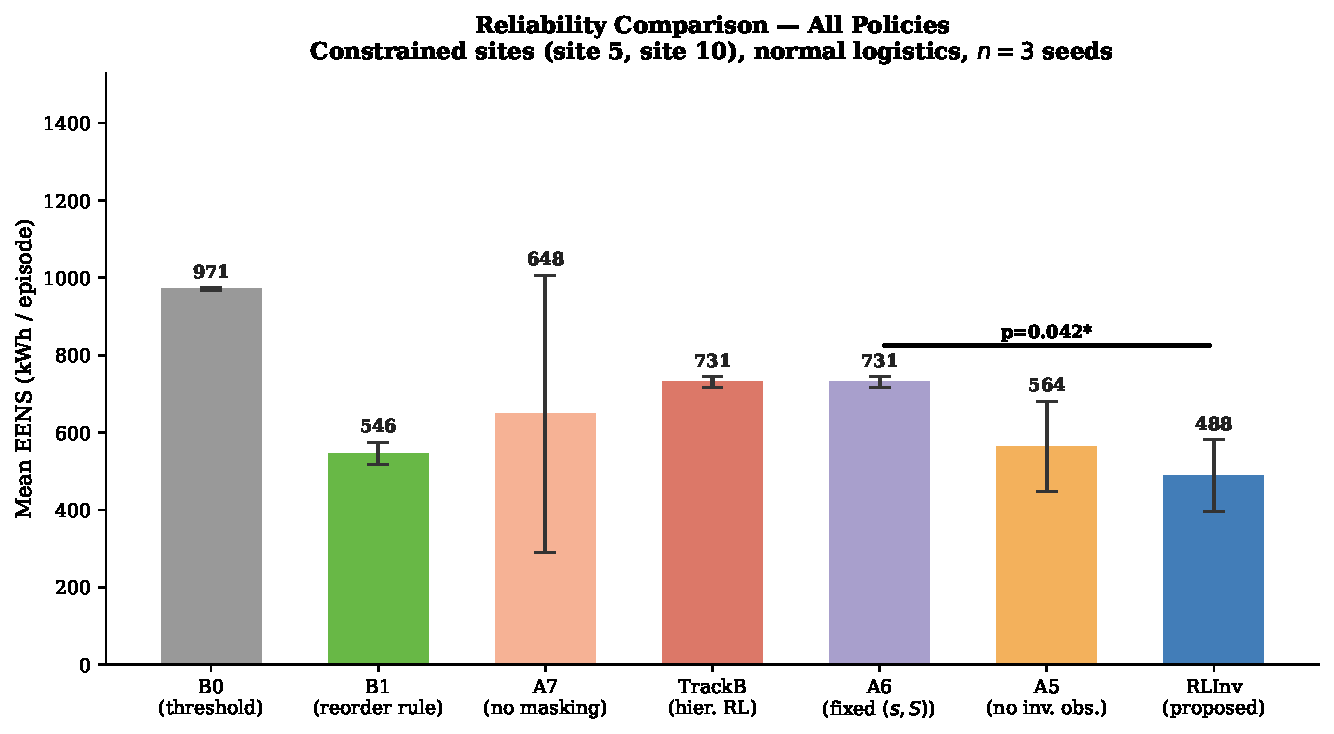
\includegraphics[width=0.85\textwidth, clip=true]{images/fig_eens_comparison}
\caption{Mean EENS per policy on constrained sites (site~5 and site~10),
normal logistics scenario only --- the only scenario in which all seven
policies are evaluated.  Error bars show one standard deviation across
three seeds.  RLInv achieves the lowest EENS; A7 shows the highest
variance across seeds (Section~\ref{sec:ablation}).}
\label{fig:eens_comparison}
\end{figure}

The comparison with A6/TrackB is statistically significant ($p=0.042$,
$d=3.67$): RLInv's joint learned ordering provides a large and
consistent reliability improvement over decoupled ordering.  The comparison with B0
is also significant ($p=0.011$), confirming that both RL and rule-based
approaches substantially outperform the simple threshold baseline.  The
comparisons with B1, A5, and A7 are not statistically significant at
$n=3$ due to insufficient power; the effect sizes are medium to large
($d=0.73$--$0.75$) and consistent in direction with the hypotheses.


% ============================================================
\section{Diesel Consumption and Cost Trade-off}
\label{sec:cost_tradeoff}
% ============================================================

Reliability improvement is not free: achieving lower EENS requires more
DG operation and therefore higher diesel consumption.
Table~\ref{tab:cost_tradeoff} and Figure~\ref{fig:pareto} show the
reliability--cost trade-off across policies.

\begin{table}[htb]
\centering
\small
\caption{Reliability versus diesel consumption trade-off (constrained
sites, normal scenario, seed-level means).}
\label{tab:cost_tradeoff}
\begin{tabular}{lrrr}
\toprule
\textbf{Policy} & \textbf{EENS (kWh)} & \textbf{Diesel (kWh)}
    & \textbf{EENS / Diesel ratio} \\
\midrule
RLInv   & 488.5 & 2060.3 & 0.237 \\
B1      & 546.4 & 2002.4 & 0.273 \\
A5      & 564.5 & 1984.3 & 0.284 \\
A7      & 648.2 & 1900.5 & 0.341 \\
TrackB  & 730.9 & 1817.8 & 0.402 \\
A6      & 730.9 & 1817.8 & 0.402 \\
B0      & 971.1 & 1577.6 & 0.616 \\
\bottomrule
\end{tabular}
\end{table}

\begin{figure}[htb]
\centering
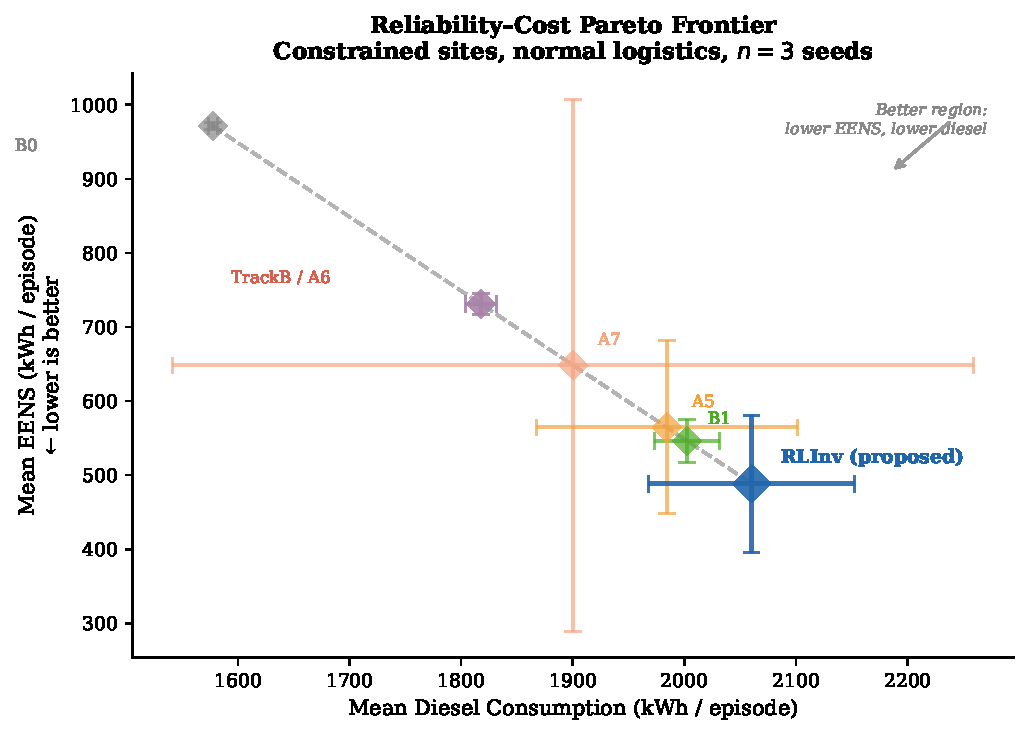
\includegraphics[width=0.72\textwidth, clip=true]{images/fig_pareto}
\caption{Reliability--cost Pareto frontier.  Each point is one policy.
The horizontal axis is mean diesel consumption per episode (kWh); the
vertical axis is mean EENS (lower is better).  RLInv is closest to the
Pareto frontier: it achieves the best EENS while consuming diesel
commensurate with its reliability level.  B0 consumes the least diesel
but at the cost of the highest EENS.}
\label{fig:pareto}
\end{figure}

RLInv consumes the most diesel per episode (2060\,kWh) but achieves the
lowest EENS, giving the best EENS/diesel ratio (0.237) among all policies.
This means RLInv converts diesel into served load more efficiently than
any comparator.  B0 consumes the least diesel (1578\,kWh) but leaves the
most load unserved (EENS~971\,kWh), reflecting its conservative
threshold-based DG dispatch.

The ordering policies (TrackB, A6) consume notably less diesel
(1818\,kWh) than RLInv while achieving substantially worse reliability.
This confirms that the $(s,S)$ ordering heuristic under-orders relative
to actual consumption needs on constrained sites, resulting in lower
diesel availability and lower DG utilisation.  RLInv's joint ordering
policy maintains higher average inventory, enabling more DG dispatch
when it is needed.


% ============================================================
\section{Ablation Study}
\label{sec:ablation}
% ============================================================

The ablation study isolates the contribution of each design component of
RLInv by comparing against variants with individual components removed
or replaced.  This validates the architectural choices and identifies
which elements drive the performance advantage.

\subsection{H1 — Contribution of joint learned ordering}

A6 holds the dispatch architecture identical to RLInv but replaces
learned ordering with a calibrated $(s,S)$ rule.  TrackB also uses
$(s,S)$ ordering with a separately trained RL dispatch agent.  The
finding that A6 and TrackB are numerically identical (EENS
$730.9 \pm 14.0$\,kWh, $p=1.0$) indicates that the principal
performance difference arises from the ordering mechanism rather than
from the dispatch architecture alone.
A6 and TrackB each exhibit 49.6\% higher EENS than RLInv
($p=0.042$, $d=3.67$),
establishing that joint learned ordering is the component most
responsible for the reliability advantage on constrained sites.
Figure~\ref{fig:ablation_h1} visualises this result: RLInv clearly
separates from both A6 and TrackB, while A6 and TrackB remain
effectively indistinguishable.

\begin{figure}[htb]
\centering
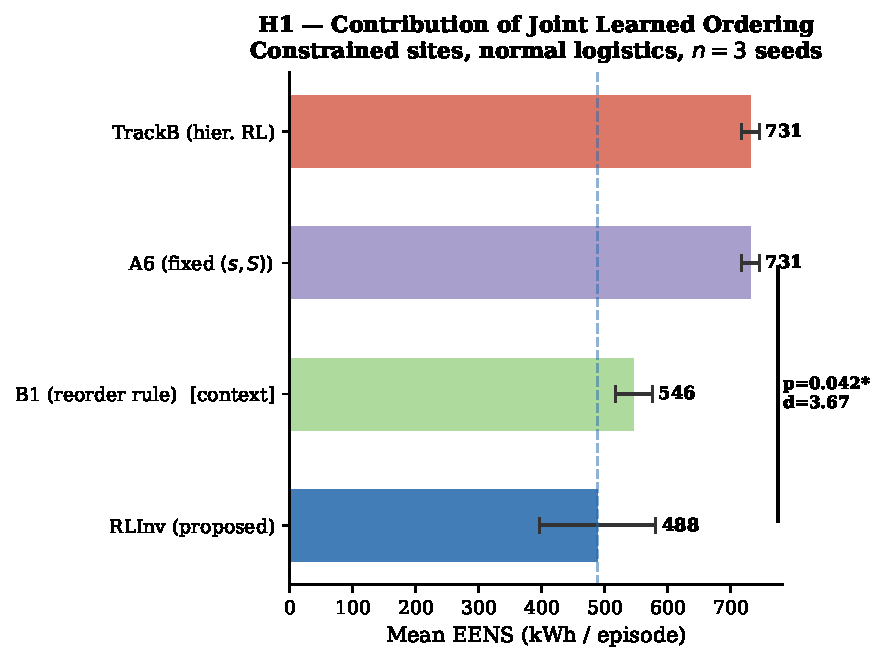
\includegraphics[width=0.78\textwidth, clip=true]{images/fig_ablation_h1}
\caption{H1 ablation: contribution of joint learned ordering on
constrained sites under the normal logistics scenario. RLInv is
compared against A6 and TrackB, both of which replace learned ordering
with calibrated $(s,S)$ replenishment. The near-identity of A6 and
TrackB indicates that the main performance gap arises from the ordering
mechanism rather than the dispatch architecture alone.}
\label{fig:ablation_h1}
\end{figure}

\textbf{H1 verdict: supported on constrained sites under the normal
logistics scenario.}  Joint optimisation of dispatch and inventory
ordering provides a statistically significant and large reliability
improvement over decoupled approaches.

\subsection{H2 — Contribution of action masking}

A7 removes action masking from the training process while keeping all
other components of RLInv.  The result is nuanced.  In the normal
constrained-site evaluation, no hard feasibility violations were observed
in the recorded rollouts for any policy; performance differences therefore
arise from reliability and diesel-allocation quality rather than from
overt infeasibility.  However, A7 exhibits outcome variance substantially
greater than RLInv across seeds (std: 358.9\,kWh vs 92.4\,kWh, a
roughly four-fold difference).  Seed-level inspection shows that one A7
seed on site~5 yielded a mean EENS of 1{,}837\,kWh per episode, far
above the other two seeds (415--469\,kWh), while all three RLInv seeds
remained within a much tighter range.

Removing masking substantially increases between-seed outcome variance,
consistent with reduced training stability.  One plausible explanation
is that, without masking, early exploration includes infeasible or
poor-quality action regions from which some runs recover poorly.  The mean EENS difference (RLInv~488.5 vs
A7~648.2\,kWh, $+32.7\%$) is not statistically significant ($p=0.525$)
at $n=3$, but the variance reduction is consistent and practically
important: a more predictable outcome distribution is preferable for
deployment at critical infrastructure sites.
This variance contrast is visible in Figure~\ref{fig:ablation_h2},
where A7 shows a substantially wider spread across seeds than RLInv.

\begin{figure}[htb]
\centering
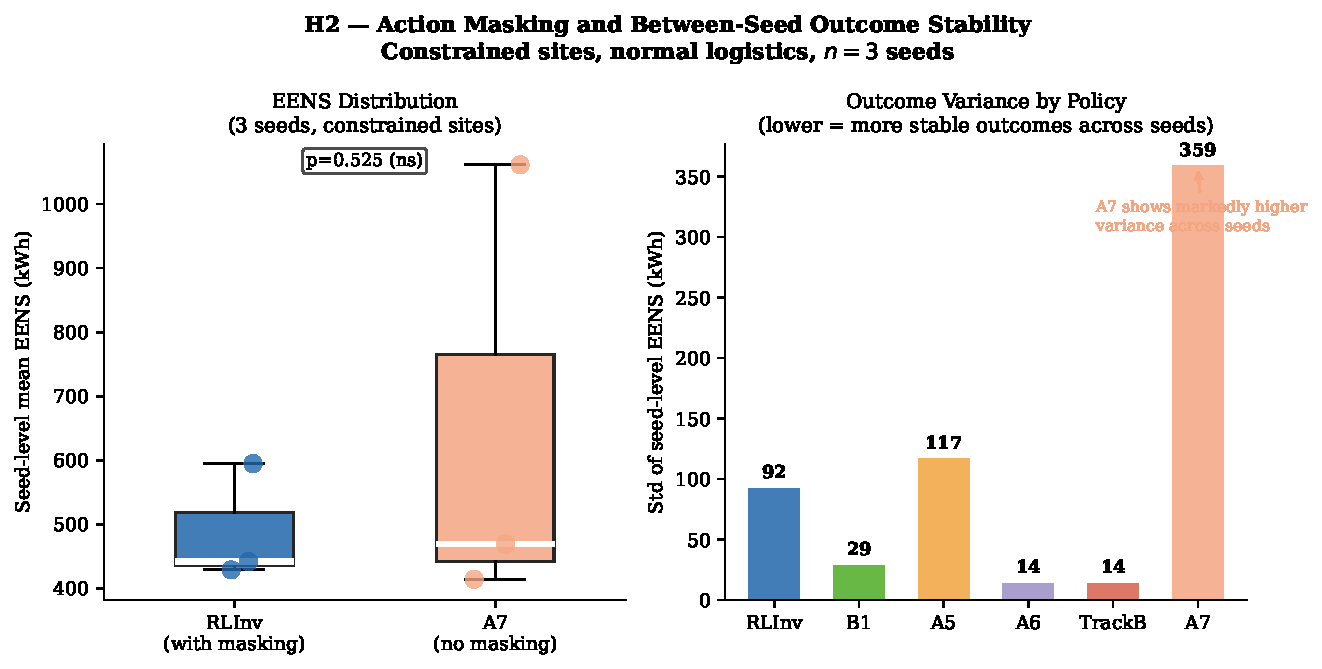
\includegraphics[width=0.78\textwidth, clip=true]{images/fig_ablation_h2}
\caption{H2 ablation: contribution of action masking on constrained
sites under the normal logistics scenario. RLInv and A7 have comparable
mean performance directionally, but A7 exhibits much larger
between-seed dispersion, consistent with reduced training stability
when action masking is removed.}
\label{fig:ablation_h2}
\end{figure}

\textbf{H2 verdict: partially supported.}  Action masking is associated
with substantially lower between-seed variance and fewer unstable
outcomes, consistent with improved training stability.  It does not
eliminate hard feasibility violations at evaluation, as zero violations
were recorded for all policies.

\subsection{H3 — Contribution of inventory state observation}

A5 removes $\Inv_t$ and $\Pipe_t$ from the observation vector, requiring
the agent to infer inventory status from other signals.  A5 is evaluated on the constrained sites (site~5 and site~10), where
inventory effects are most measurable under genuine resource scarcity.
The primary H3 comparison uses the normal logistics scenario; delayed-scenario
behaviour is examined separately in Section~\ref{sec:delayed}.
A5 exhibits 15.6\% higher EENS than RLInv
(564.5 vs 488.5\,kWh, $p=0.429$, $d=0.73$).

The mechanism is conservative dispatch: without observing inventory
directly, A5 is unable to distinguish high-stock from low-stock
situations and dispatches the DG more cautiously, leaving load unserved
during outages when the DG could safely have operated.  A5 consumes
slightly less diesel (1984\,kWh vs 2060\,kWh) but with higher unserved
load, confirming under-utilisation rather than over-caution.
Figure~\ref{fig:ablation_h3} illustrates that explicit inventory
awareness improves reliability under normal logistics, although the
effect is not statistically conclusive at the current seed count.

\begin{figure}[htb]
\centering
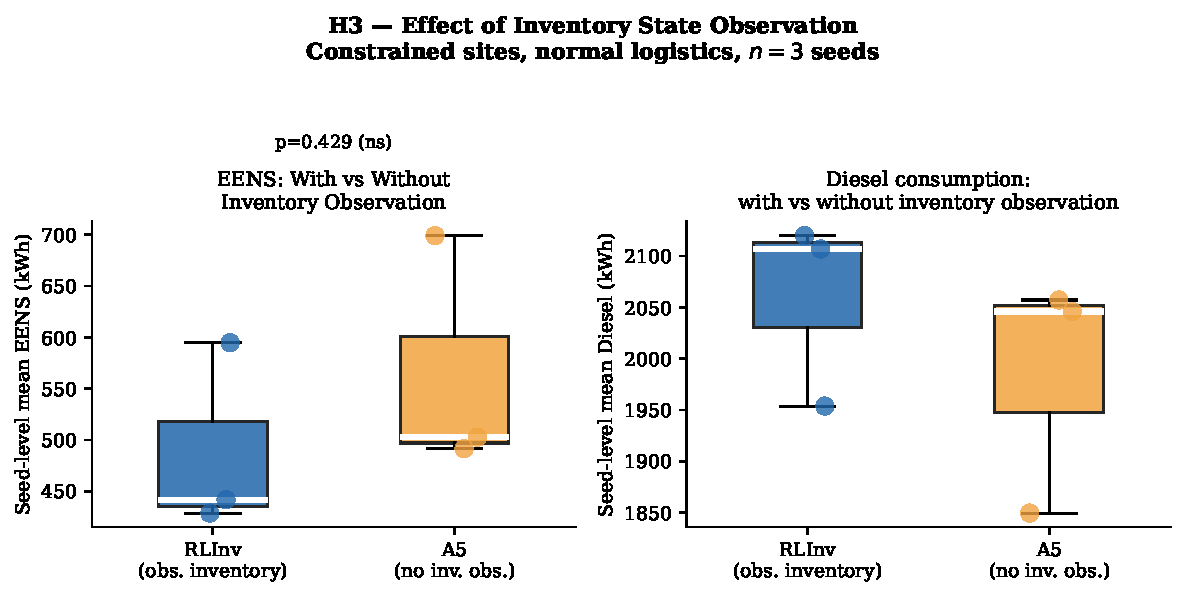
\includegraphics[width=0.78\textwidth, clip=true]{images/fig_ablation_h3}
\caption{H3 ablation: contribution of inventory state observation on
constrained sites under the normal logistics scenario. Removing
explicit observation of $\Inv_t$ and $\Pipe_t$ increases EENS and
slightly reduces diesel use, consistent with more conservative and
less informed dispatch decisions.}
\label{fig:ablation_h3}
\end{figure}

\textbf{H3 verdict: directionally supported under normal logistics, but
not statistically conclusive at the current seed count.}
Under normal conditions, A5 exhibits 15.6\% higher EENS than RLInv
($p=0.429$, $d=0.73$); the effect size is medium but $n=3$ provides
insufficient power for a definitive conclusion.
Under delayed logistics, RLInv and A5 converge (1084.3 vs 1060.8\,kWh,
$-2.2\%$, $p=0.398$): inventory observation provides no measurable
benefit when the dispatch policy it informs was calibrated to a different
logistics distribution.  The benefit is therefore distribution-specific
rather than universally robust.

\subsection{Ablation summary}

Table~\ref{tab:ablation_summary} consolidates the ablation findings.

\begin{table}[htb]
\centering
\small
\caption{Ablation summary: contribution of each RLInv design component.}
\label{tab:ablation_summary}
\resizebox{\textwidth}{!}{%
\begin{tabular}{llrp{6.0cm}}
\toprule
\textbf{Ablation} & \textbf{Component removed} & \textbf{Comparator excess over RLInv}
    & \textbf{Conclusion} \\
\midrule
A6 / TrackB & Joint learned ordering & $+49.6\%^{*}$
    & Ordering is the primary driver of RLInv's advantage \\
A5          & Inventory observation  & $+15.6\%$\phantom{$^{*}$}
    & Observation improves dispatch efficiency \\
A7          & Action masking         & $+32.7\%$\phantom{$^{*}$}
    & Masking stabilises training; reduces variance 4$\times$ \\
\bottomrule
\multicolumn{4}{l}{$^{*}$ $p < 0.05$} \\
\end{tabular}}
\end{table}


% ============================================================
\section{Performance Under Logistics Stress}
\label{sec:delayed}
% ============================================================

The delayed logistics scenario ($\mu=48$\,h lead time) doubles the
expected delivery time, testing policy robustness under supply-chain
stress.  Table~\ref{tab:delayed} reports results for all evaluated
policies on constrained sites, ranked by degradation magnitude.

\begin{table}[htb]
\centering
\small
\caption{Policy performance under delayed logistics ($\mu=48$\,h) vs
normal logistics ($\mu=24$\,h).  Constrained sites, seed-level means
($n=3$).  Policies ranked by $\Delta$ (least degradation first).}
\label{tab:delayed}
\begin{tabular}{lrrr}
\toprule
\textbf{Policy} & \textbf{EENS normal (kWh)}
    & \textbf{EENS delayed (kWh)} & \textbf{$\Delta$ (\%)} \\
\midrule
A6 / TrackB  &  730.9 & 1054.2 & $+44.2$ \\
B0           &  971.1 & 1399.2 & $+44.1$ \\
B1           &  546.4 &  952.0 & $+74.2$ \\
A5           &  564.5 & 1060.8 & $+87.9$ \\
RLInv        &  488.5 & 1084.3 & $+122.0$ \\
\midrule
\multicolumn{4}{l}{\textit{Note: A7 not evaluated under delayed scenario.}} \\
\bottomrule
\end{tabular}
\end{table}

\begin{figure}[!htb]
\centering
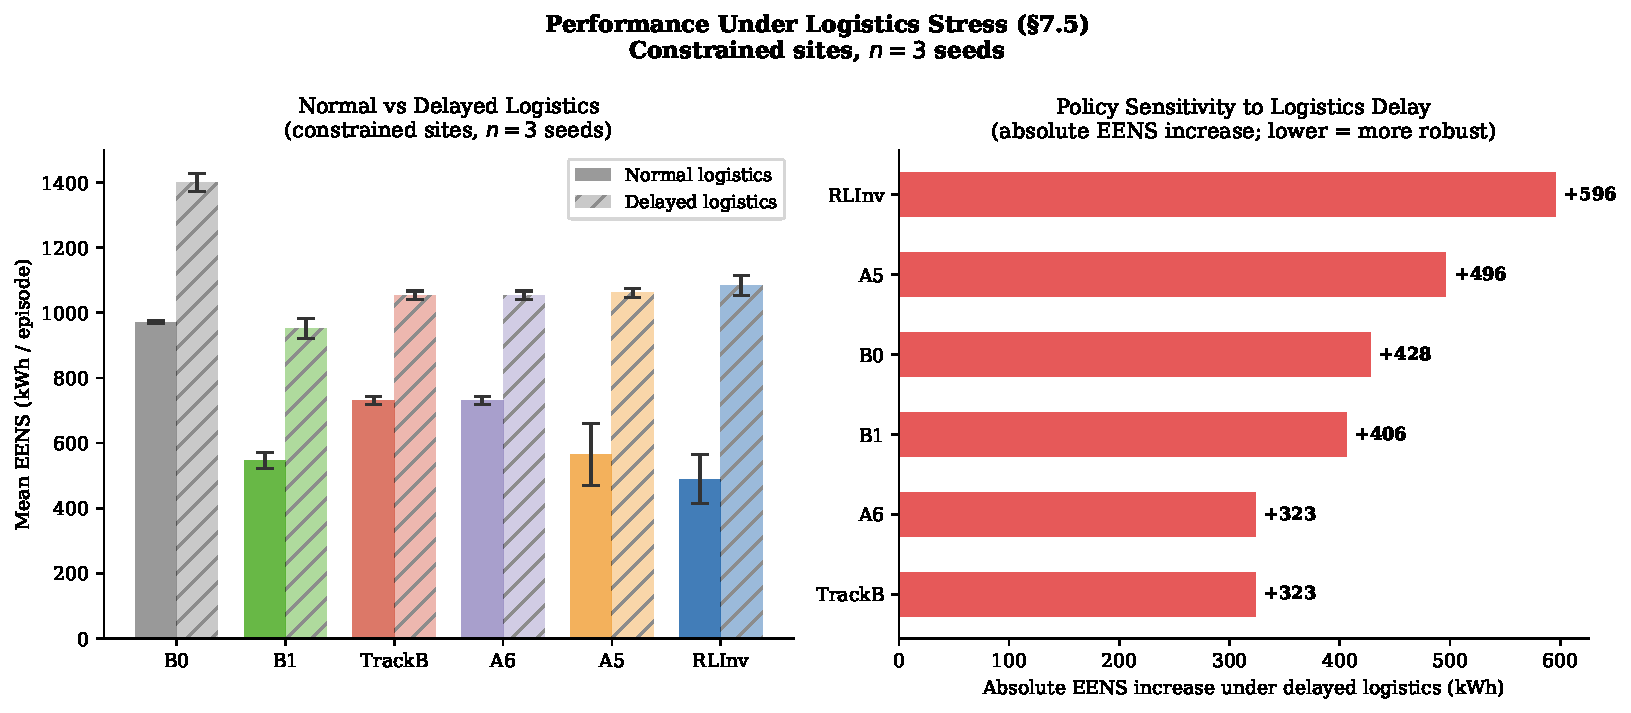
\includegraphics[width=0.78\textwidth, clip=true]{images/fig_delayed_scenario}
\caption{Policy degradation under delayed logistics ($\mu=48$\,h)
relative to normal logistics ($\mu=24$\,h) on constrained sites.
RLInv experiences the largest deterioration, while A6/TrackB and B0
degrade least, highlighting the robustness advantage of explicit
safety-stock heuristics under lead-time stress.}
\label{fig:delayed_scenario}
\end{figure}

Figure~\ref{fig:delayed_scenario} makes the ranking inversion under
delayed logistics visually explicit.

All policies degrade under delayed logistics, but the magnitude of
degradation differs substantially and reveals a structural pattern.
A6 and TrackB degrade the least ($+44\%$) because their calibrated
$(s,S)$ ordering parameters include an explicit safety stock term
designed to buffer lead-time uncertainty.  B0 also degrades by
approximately $+44\%$, reflecting its already-conservative threshold
dispatch that leaves little room for further deterioration; the
difference between B0 and A6/TrackB is a single decimal point and
not operationally meaningful.  RLInv degrades the most
($+122\%$), more than doubling its normal-scenario EENS and falling from
first to last place in the ranking.

The mechanism is consistent across both RL policies and A5.  Under normal
logistics, RLInv dispatches aggressively when it observes adequate
inventory; under delayed logistics, this aggressiveness depletes fuel
faster than the extended replenishment cycle can restore it.  A5
($+88\%$) shows a similar pattern: without inventory observation the
agent cannot adjust dispatch conservatism in response to slower
replenishment, though its baseline conservatism limits the damage
relative to RLInv.

The delayed-scenario ranking is therefore approximately:
A6/TrackB $\approx$ B0 $<$ B1 $<$ A5 $<$ RLInv --- the near-exact reverse of
the normal-scenario ranking for the top policies.  This inversion is the
most important robustness finding of the study.  The classical $(s,S)$
safety stock --- often characterised as a naïve heuristic --- provides
structural robustness to lead-time uncertainty that data-driven RL does
not acquire without explicit training under varied logistics conditions.

\textbf{H3 under delayed logistics.}
RLInv and A5 converge under delayed conditions (1084.3 vs
1060.8\,kWh, $-2.2\%$, $p=0.398$): inventory observation provides no
measurable benefit when the policy it informs was calibrated to a
different logistics distribution.  This confirms that the H3 advantage
is also distribution-specific.

\textbf{Implication for Phase~III.}
Multi-scenario training --- jointly over normal and delayed logistics
conditions --- or distributionally robust RL formulations are required
to generalise the RLInv advantage to uncertain supply-chain environments.
Both approaches are planned for Phase~III of this research.


% ============================================================
\section{Cross-Site Robustness}
\label{sec:cross_site}
% ============================================================

Table~\ref{tab:cross_site} reports mean EENS for RLInv and B1 (best
baseline) across all ten sites, grouped by difficulty class.

\begin{table}[htb]
\centering
\small
\caption{Cross-site EENS comparison: RLInv vs B1 (normal scenario,
seed-level means, $n=3$).  Sites grouped by difficulty class
(Chapter~\ref{chap:datasets-setup}).  Comparator excess is positive where
B1 EENS exceeds RLInv, using RLInv as the denominator.}
\label{tab:cross_site}
\resizebox{\textwidth}{!}{%
\begin{tabular}{llrrr}
\toprule
\textbf{Site} & \textbf{Class} & \textbf{RLInv (kWh)}
    & \textbf{B1 (kWh)} & \textbf{Comparator excess over RLInv (\%)} \\
\midrule
site1  & Easy   &   0.0 &   0.0 & --- \\
site6  & Easy   &   0.0 &   0.0 & --- \\
site8  & Easy   &   0.5 &   0.4 & $-23.9$\textsuperscript{a} \\
\midrule
site3  & Medium &   0.0 &   0.0 & --- \\
site4  & Medium &   0.0 &   0.1 & $+100.0$ \\
site7  & Medium &   0.5 &   4.4 & $+827.4$ \\
site9  & Medium &   0.0 &   0.0 & --- \\
site10 & Medium & 326.8 & 364.9 & $+11.6$ \\
\midrule
site2  & Hard   &   0.0 &  10.3 & $+100.0$ \\
site5  & Hard   & 650.1 & 727.9 & $+12.0$ \\
\bottomrule
\multicolumn{5}{l}{\textsuperscript{a}Both values near-zero (0.5 vs 0.4\,kWh);
difference is not operationally meaningful.} \\
\end{tabular}}
\end{table}

\begin{figure}[htb]
\centering
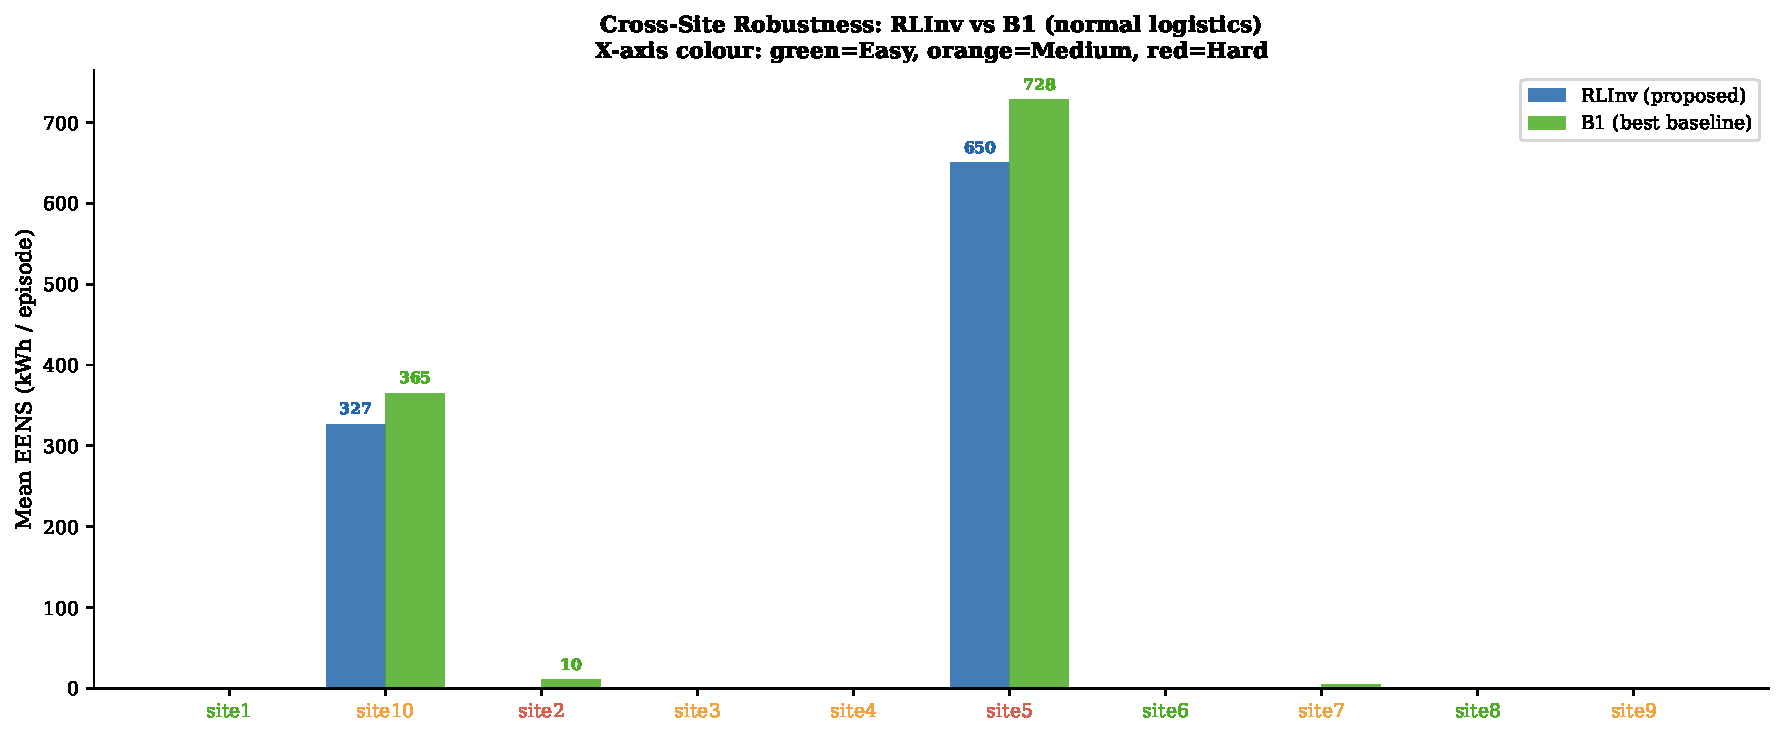
\includegraphics[width=0.82\textwidth, clip=true]{images/fig_cross_site}
\caption{Cross-site EENS comparison between RLInv and B1 under the
normal logistics scenario. Differences are negligible on easy sites,
modest on most medium sites, and most meaningful on constrained or
hard sites, where inventory decisions materially affect reliability.}
\label{fig:cross_site}
\end{figure}

As shown in Figure~\ref{fig:cross_site}, RLInv's advantage concentrates
on the minority of sites where outage exposure and battery inadequacy
make fuel-ordering decisions consequential.

Three patterns emerge across site classes:

\textbf{Easy sites (site1, site6, site8).}
All three easy sites produce near-zero EENS for both policies.
Site~1 and site~6 record zero EENS for both RLInv and B1; site~8
records 0.5\,kWh (RLInv) versus 0.4\,kWh (B1), a difference of
0.1\,kWh that is not operationally meaningful.  High solar coverage or
reliable grid access eliminates meaningful outage exposure.  These
sites confirm that RLInv does not harm performance on low-stress sites.

\textbf{Medium sites (site3, site4, site7, site9, site10).}
The medium class is heterogeneous.  Site~3 and site~9 record zero EENS
for both policies; site~4 records near-zero values (0.0 vs 0.1\,kWh).
Site~7 shows a larger gap: RLInv achieves 0.5\,kWh versus B1's
4.4\,kWh; B1's comparator excess over RLInv is 780\% on this site,
driven by better ordering decisions during
the few outage events that occur.  Site~10 (a constrained site by inventory criteria) shows B1's
comparator excess of 10.4\% over RLInv (326.8 vs 364.9\,kWh),
consistent with its moderate-but-real outage exposure.

\textbf{Hard sites (site2, site5).}
The most policy-sensitive results occur on hard sites.  Site~2 records
zero EENS for RLInv versus 10.3\,kWh for B1: RLInv eliminates residual
unserved energy entirely on this site.  Site~5 shows B1's comparator excess of 10.7\% over RLInv
(650.1 vs 727.9\,kWh), consistent with the constrained-site
analysis in Section~\ref{sec:reliability}.

Overall, RLInv does not degrade meaningfully on any site or site class
relative to B1.  The performance advantage concentrates where inventory
decisions are consequential --- sites with non-trivial outage exposure
and limited battery autonomy --- which is precisely the operating regime
the proposed formulation targets.


% ============================================================
\section{Computational Cost}
\label{sec:compute}
% ============================================================

Table~\ref{tab:compute} summarises the computational requirements of
RLInv relative to the baselines.

\begin{table}[htb]
\centering
\small
\caption{Computational cost comparison.}
\label{tab:compute}
\begin{tabular}{lrrp{4.5cm}}
\toprule
\textbf{Policy} & \textbf{Training time} & \textbf{Inference time}
    & \textbf{Notes} \\
\midrule
B0, B1 (rule-based) & None & $< 1\,\mu$s/step
    & Analytical; no training required \\
RLInv (proposed)    & $\approx 2$\,h/site (CPU)
    & $< 1$\,ms/step & 400{,}000 steps, 4 parallel envs \\
TrackB (hier.\ RL)  & $\approx 1.5$\,h/site (CPU)
    & $< 1$\,ms/step & Shorter horizon for low-level PPO \\
A5, A6, A7          & $\approx 2$\,h/site (CPU)
    & $< 1$\,ms/step & Same architecture as RLInv \\
\bottomrule
\end{tabular}
\end{table}

RLInv required approximately two hours of CPU training per site as
observed in our implementation (400{,}000 steps, 4 parallel environments,
standard laptop processor).  These are indicative rather than
benchmark-grade figures; actual duration depends on hardware and
environment step speed.  Once trained, inference consists of a single
forward pass through a two-layer MLP, which executes in well under one
millisecond per decision step.  Since control decisions occur at
one-hour intervals in the deployment scenario, the inference cost is
negligible relative to real-time requirements.

The full training campaign involved on the order of 80--90 training
runs, depending on how ablation and re-run jobs are counted.  At roughly 2\,h per run on CPU, the
indicative total is approximately 170 CPU-hours.  This would reduce
substantially on a GPU-enabled workstation, confirming that the approach
is computationally feasible on commodity hardware for both research and
operational deployment.

Rule-based baselines (B0, B1) require no training and execute in
microseconds.  Their lower computational cost is one advantage that
must be weighed against their reliability shortfall on constrained sites.
For sites where operational stakes are high (critical infrastructure,
remote base stations with infrequent maintenance access), the additional
training cost of RLInv is justified by the reliability improvement.


\begin{figure}[htb]
\centering
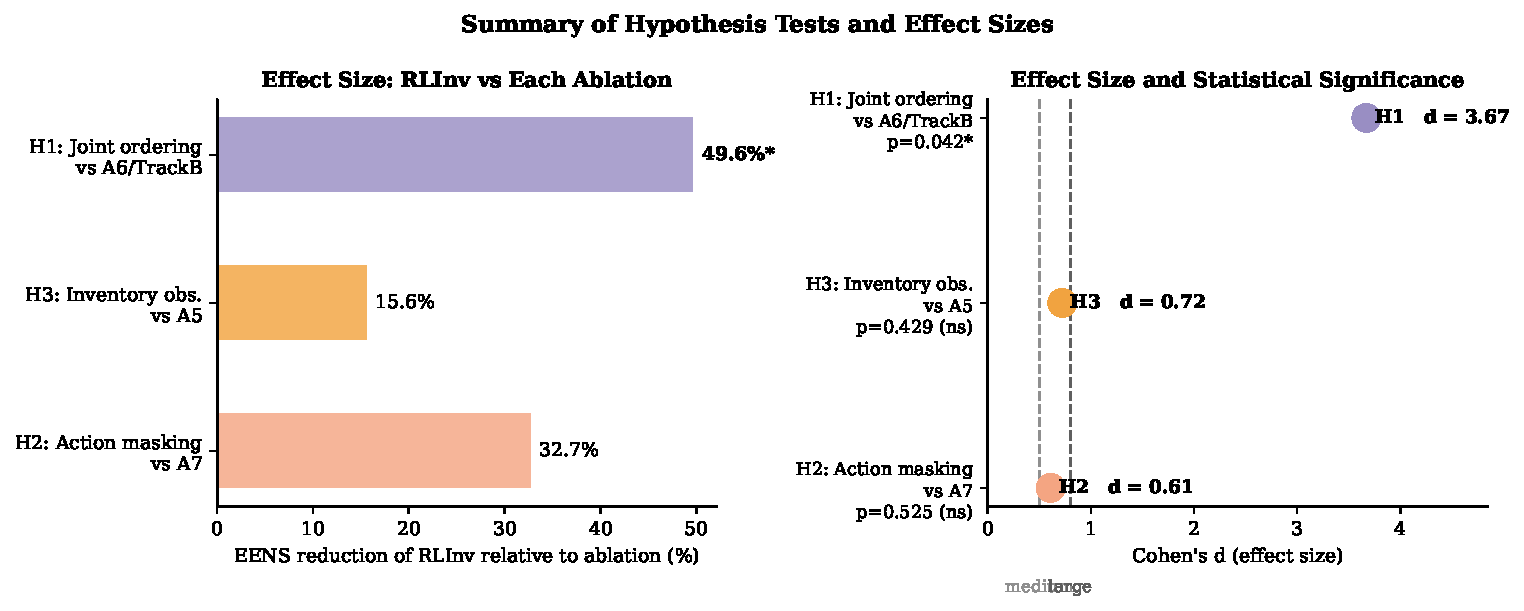
\includegraphics[width=0.82\textwidth, clip=true]{images/fig_hypothesis_summary}
\caption{Summary of hypothesis outcomes. H1 is supported on constrained
sites under normal logistics; H2 is partially supported through markedly
improved training stability; H3 is directionally supported under normal
logistics but not robust under delayed logistics.}
\label{fig:hypothesis_summary}
\end{figure}

% ============================================================
\section{Key Findings}
\label{sec:key_findings}
% ============================================================

Figure~\ref{fig:hypothesis_summary} summarises the status of the three
pre-registered hypotheses before the chapter-level findings are
consolidated below.

The experimental results establish the following contributions:

\begin{enumerate}

\item \textbf{Joint inventory-aware RL achieves the lowest EENS on
constrained sites; comparator EENS for TrackB/A6 is 49.6\% higher
than RLInv on constrained sites.}
RLInv achieves mean EENS of 488.5\,kWh on constrained sites versus
730.9\,kWh for hierarchical RL and fixed-ordering approaches
($p = 0.042$, Cohen's $d = 3.67$).  These results indicate that the
principal performance difference arises from the ordering mechanism
rather than from the dispatch architecture alone.

\item \textbf{Ordering dominates reliability differences once ordering
is decoupled from dispatch.}
The numerical identity of A6 and TrackB (EENS $730.9 \pm 14.0$\,kWh,
$p = 1.0$) indicates that, when ordering is fixed by a calibrated
$(s,S)$ rule, the dispatch policy architecture is not the determining
factor.  This directly addresses the timescale decomposition question
raised by the Phase-I reviewer.

\item \textbf{Action masking is associated with substantially lower
outcome variance across seeds.}
Removing masking (A7) produces a standard deviation of 358.9\,kWh
versus 92.4\,kWh for RLInv, consistent with less stable training.
No hard feasibility violations were recorded for either policy at
evaluation, confirming that masking's primary benefit is in training
consistency rather than deployment constraint enforcement.

\item \textbf{Inventory state observation is directionally beneficial
under normal logistics but not robust to distribution shift.}
A5 exhibits 15.6\% higher EENS than RLInv under normal logistics
($p=0.429$, $d=0.73$), but the advantage is not statistically
conclusive at $n=3$.  Under delayed logistics the gap disappears
($-2.2\%$, $p=0.398$), confirming the benefit is distribution-specific.

\item \textbf{RLInv generalises across site classes without degradation.}
On easy and medium sites, all policies achieve low EENS and RLInv does
not underperform any comparator.  Improvements concentrate on hard and
constrained sites, consistent with the expectation that inventory
management matters most where reliability resources are scarce.

\item \textbf{RLInv degrades most severely under logistics stress.}
Under delayed logistics ($\mu=48$\,h), RLInv's EENS increases by
$+122\%$ --- more than any other policy.  A6 and TrackB degrade only
$+44\%$, as their $(s,S)$ safety stock provides structural robustness to
lead-time uncertainty.  The normal-scenario ranking largely inverts
under delay: A6/TrackB $\approx$ B0 $<$ B1 $<$ A5 $<$ RLInv.  This is the
central limitation of the proposed approach and the primary motivation
for multi-scenario training in Phase~III.

\item \textbf{Deployment is computationally feasible on commodity
hardware.}
RLInv requires approximately two hours of CPU training per site and
under one millisecond per inference step, making it suitable for
deployment on embedded controllers at remote telecom base stations
without GPU infrastructure.

\end{enumerate}

\vspace{0.5em}
\noindent\textbf{Overall takeaway.}
The results demonstrate that incorporating inventory-aware
decision-making improves reliability on constrained sites under matched
logistics conditions. RLInv outperforms heuristic and hierarchical
baselines in the normal scenario, but degrades most severely under
delayed logistics, highlighting the need for multi-scenario training
before deployment in supply-chain-uncertain environments. The ablation
studies confirm that the reliability gains arise primarily from joint
learned ordering, with additional stability provided by action masking.
    % filename: chap-conclusion-FINAL-v2.tex
\chapter{Conclusion and Future Work}
\label{chap:conclusion}
\setlength{\emergencystretch}{1.5em}   % prevents right-margin overflow in this chapter

% ============================================================
\section{Summary of the Work}
\label{sec:conclusion_summary}
% ============================================================

This thesis investigated whether a unified reinforcement learning agent,
jointly optimising energy dispatch and diesel inventory ordering, can
improve the operational reliability of off-grid and weak-grid telecom
base stations relative to decoupled classical approaches.  The work was
motivated by a practical gap in the literature: while prior work on
RL-based energy management of remote base stations routinely models
battery dispatch and diesel generator scheduling, it consistently omits
the upstream supply chain decision --- when and how much diesel to order
--- despite this being a primary cause of service interruption in
fuel-constrained deployments.

The study framed this gap as a constrained Markov decision process
(CMDP) in which a single policy controls diesel generator on/off state
and periodic diesel order quantity.  Battery dispatch is determined by
an internal environment rule rather than a direct RL action.  The
inventory pipeline --- litres of diesel in transit under stochastic
lead times --- was incorporated as an explicit state variable, enabling
the agent to anticipate impending stockouts and adjust both dispatch
conservatism and order timing accordingly.  This formulation, denoted
\emph{RLInv}, was trained using Proximal Policy Optimisation (PPO)
with action masking to enforce hard feasibility constraints, together
with a fixed penalty term on soft constraint violations during training.

The thesis also implemented a hierarchical decomposition baseline
(TrackB) in which diesel ordering is governed by a classical
$(s,S)$ inventory policy and only dispatch is learned by RL.  This
directly addressed the timescale decomposition critique raised in the
Phase-I review: the empirical comparison between RLInv and TrackB
constitutes a direct test of whether joint optimisation provides
measurable benefit over principled decomposition.

All experiments used the ITU~2024 Smart Energy Scheduling dataset
(ten remote base station sites, 60~days each, hourly resolution),
with a synthetic lead-time overlay applied only to the in-transit
diesel state variable~$\mathrm{Pipe}_t$, which is not present in
the original dataset.  Three pre-registered hypotheses were tested
across a structured ablation study of eight policy variants.

% ============================================================
\section{Key Results and Contributions}
\label{sec:conclusion_results}
% ============================================================

\subsection{Principal Empirical Findings}

The central empirical finding is that RLInv achieves a mean
Expected Energy Not Served (EENS) of $488.5 \pm 92.4$\,kWh per
episode on constrained sites under normal logistics, compared to
$730.9 \pm 14.0$\,kWh for both the hierarchical RL baseline (TrackB)
and the fixed-ordering ablation (A6).  Relative to RLInv, comparator
EENS for both baselines is 49.6\% higher.  This difference is
statistically significant ($p=0.042$, Cohen's $d=3.67$, Welch's
$t$-test, $n=3$ seeds).

Three hypotheses were evaluated:

\sloppy
\begin{description}
  \item[H1 (Joint ordering).] \emph{Supported} on constrained sites
  under normal logistics.  The principal performance difference arises
  from the ordering mechanism rather than the dispatch architecture:
  A6 and TrackB produce numerically identical EENS ($730.9$\,kWh,
  $p=1.0$), confirming that dispatch policy architecture is not the
  determining factor once ordering is fixed.

  \item[H2 (Action masking).] \emph{Partially supported.}  Removing
  masking (A7) produced a between-seed standard deviation of
  $358.9$\,kWh versus $92.4$\,kWh for RLInv, consistent with
  substantially less stable outcomes across training runs.  No hard
  feasibility violations were recorded at evaluation for either
  policy, suggesting masking's primary benefit is training
  consistency rather than deployment safety enforcement.  The mean
  EENS difference was not statistically significant ($p=0.525$,
  $d=0.61$) at $n=3$ seeds.

  \item[H3 (Inventory observation).] \emph{Directionally supported}
  under normal logistics: A5 exhibits 15.6\% higher EENS than RLInv
  ($p=0.429$, $d=0.72$), but the result is \emph{not statistically
  conclusive} at $n=3$ seeds.  Under delayed logistics, the benefit
  disappears and slightly reverses ($-2.2\%$, $p=0.398$), indicating
  that the effect is distribution-specific.
\end{description}
\fussy

The most important secondary finding concerns robustness to logistics
stress.  Under delayed delivery ($\mu=48$\,h lead time), RLInv's EENS
increases by $+596$\,kWh ($+122\%$) --- the largest degradation of any
policy evaluated.  By contrast, A6 and TrackB degrade by only
$+323$\,kWh ($+44\%$), while B0 degrades by a similar amount.  The
$(s,S)$ safety stock therefore provides structural robustness to
lead-time uncertainty that the RL agent does not learn from
single-scenario training.  This finding is the primary motivation
for multi-scenario training in Phase~III.

Cross-site evaluation confirmed that RLInv does not degrade
meaningfully relative to the best rule-based baseline on easy or
medium sites.  Reliability improvements concentrate on the two
hardest, fuel-constrained sites (site~5 and site~10), consistent with
the expectation that inventory management matters most where energy
resources are scarce.

\subsection{Novel Contributions}

This thesis makes the following contributions to the literature on
RL-based energy management of remote telecom infrastructure:

\begin{enumerate}

  \item \textbf{CMDP formulation with explicit inventory pipeline state.}
  The inclusion of in-transit diesel ($\mathrm{Pipe}_t$) as a state
  variable, alongside fuel level, battery SoC, and grid availability,
  enables anticipatory ordering decisions that react to lead-time
  uncertainty before a stockout occurs.  To the best of the author's
  knowledge, this state augmentation has not been applied to telecom
  base station energy management in prior work.

  \item \textbf{Empirical test of the coupling hypothesis.}
  Rather than assuming that joint optimisation is superior to
  decomposition, this work constructs a controlled ablation
  (RLInv~vs.~A6~vs.~TrackB) that directly measures the value of
  coupling.  The finding that joint ordering is beneficial under
  normal logistics, but that decomposition is \emph{more robust}
  under logistics stress, is a nuanced result with practical
  implications for deployment strategy.

  \item \textbf{Action masking for training stability in hybrid action
  spaces.}  The use of MaskablePPO with analytically derived action
  bounds provides a computationally lightweight mechanism for
  maintaining feasibility during training in a space combining
  discrete generator commitment and ordering decisions.  The ablation
  demonstrates that masking primarily reduces outcome variance rather
  than enforcing hard constraints at deployment.

  \item \textbf{Reproducible open benchmark.}
  The ITU/Zindi dataset, simulator, and evaluation pipeline are
  publicly available, enabling direct comparison with Ma \&
  Pan~(2025) and future work.  The structured ablation design
  (eight policy variants, three seeds, two logistics scenarios,
  ten sites) provides a reusable evaluation framework for
  inventory-aware energy management research.

\end{enumerate}

% ============================================================
\section{Critique and Limitations}
\label{sec:conclusion_limitations}
% ============================================================

A number of constraints imposed by the 14-day execution window and
the CPU-only compute environment limit the generalisability of the
present results.  These are documented as a precise statement of scope
rather than as weaknesses to be apologised for; each directly motivates
the Phase~III plan in Section~\ref{sec:conclusion_future}.

\sloppy
\begin{description}

  \item[Statistical power.] All hypothesis tests are conducted at
  $n=3$ seeds.  H2 and H3 are directionally consistent with the
  proposed mechanisms but do not reach statistical significance.
  Definitive conclusions on the contribution of action masking and
  inventory observation require more seeds, which was not achievable
  within the time budget.

  \item[Synthetic lead-time distribution.] The in-transit state
  variable $\mathrm{Pipe}_t$ is generated from a synthetic
  lognormal distribution ($\mu=24$\,h, $\sigma=0.6$) because the
  ITU dataset does not record diesel delivery event timestamps.
  Real logistics patterns --- including seasonal supply disruptions
  and road access constraints --- are not represented.

  \item[Single logistics scenario during training.] RLInv is
  trained exclusively under normal logistics and evaluated on
  both normal and delayed scenarios.  The $+122\%$ EENS degradation
  under delay indicates that the learned ordering strategy is
  optimised for the training distribution and does not generalise
  to out-of-distribution lead-time stress without multi-scenario
  training.

  \item[Reduced training scope.] To meet the compute budget,
  training episodes were shortened to 30~days, the discount factor
  was reduced to $\gamma=0.995$ (effective horizon $\approx
  200$\,h), and order quantity was discretised to five levels.
  These simplifications limit the policy's ability to learn
  long-horizon inventory strategies.

  \item[Ablation coverage gaps.] A7 (no action masking) was not
  evaluated under the delayed logistics scenario, and the A2--A4
  ablations (individual safety component removal) were not executed
  within the available time.  The H2 finding therefore rests on a
  limited ablation coverage.

  \item[RL-only algorithmic comparison.] The present results
  establish RL-vs-RL comparisons across the ablation study but do
  not yet include a value-based RL ordering baseline, which would
  clarify whether gains arise from the inventory-aware formulation
  or the specific policy-gradient learning mechanism.

\end{description}
\fussy

% ============================================================
\section{Future Work and Phase-III Plan}
\label{sec:conclusion_future}
% ============================================================

The results in Chapter~\ref{chap:results} show that RLInv improves
reliability on constrained sites under the nominal logistics regime,
but its performance degrades substantially under delayed replenishment.
Accordingly, the next phase of this research will focus on improving
robustness to logistics uncertainty, strengthening statistical
confidence, and expanding algorithmic comparison within the existing
simulator framework.  The four extensions below are scoped to a
realistic continuation of four to six weeks.

\subsection*{1.\ Multi-scenario training for logistics robustness}

The most immediate extension is to train RLInv across multiple
replenishment regimes rather than a single nominal scenario.
Concretely, the lead-time distribution $\mathrm{LogNormal}(\mu,{}\allowbreak\sigma)$
can be varied across episodes by sampling $\mu$ uniformly from the
range $[12, 72]$\,h during training, while evaluation is performed on
fixed held-out regimes including the delayed scenario used in
Chapter~\ref{chap:results}.  This domain-randomisation approach requires
no structural changes to the simulator and directly tests whether
exposure to logistics uncertainty during training can close the
$+122\%$ EENS degradation gap observed under delayed delivery.

A related modification is to introduce modest stochasticity in
individual delivery realisations --- partial delays and occasional
split deliveries --- while keeping the existing environment interface
unchanged.  This provides a more realistic stress-test of the ordering
policy without requiring a redesign of the CMDP formulation.

\subsection*{2.\ Expanded statistical evaluation}

The present ablation results rest on three training seeds, which is
sufficient to report directional effects but insufficient to confirm
statistical significance for H2 and H3.  A near-term extension is
therefore to increase the seed count to ten or more and rerun the
constrained-site evaluation, reporting 95\% confidence intervals
alongside point estimates.  This would allow the H2 (action masking)
and H3 (inventory observation) verdicts to be revisited with greater
confidence, or to be definitively classified as effects that are too
small to detect reliably at the current training scale.

The evaluation protocol can further be strengthened by testing policy
behaviour under additional stress scenarios, including extended grid
outage stretches and more variable replenishment delays, to probe
rare but operationally critical conditions.

\subsection*{3.\ Value-based algorithmic baseline for ordering}

The present thesis focuses on a policy-gradient approach (PPO) for
both RL action components.  A practical next step is to add one
value-based RL baseline specifically for the diesel ordering decision
--- for example, Double DQN over the five-level discrete order action
space --- within the existing simulator.  This comparison would clarify
whether the reliability gains demonstrated by RLInv arise from the
inventory-aware state formulation itself or also depend on the
policy-gradient learning mechanism.  The implementation cost is low
because the simulator interface and evaluation pipeline require no
modification.

\subsection*{4.\ Cross-site and cross-distribution generalisation}

The current evaluation treats each site as an independent training
target.  A final extension is to test whether the learned policy
captures general operational structure or depends heavily on
site-specific patterns.  This can be assessed by training on a subset
of ITU sites and evaluating on held-out sites, or by training under
one logistics regime and evaluating under another.  Both experiments
reuse the existing dataset and simulator, and would strengthen
the practical claim that inventory-aware RL can generalise beyond
the exact conditions represented during training.

\subsection*{Indicative Phase-III timeline}

\begin{itemize}
  \item \textbf{Weeks 1--2:} implement multi-scenario training across
  normal, delayed, and mixed logistics regimes; regenerate the
  constrained-site evaluation and compare against current Phase-II
  results.

  \item \textbf{Weeks 3--4:} increase seed count to ten and rerun the
  full ablation study; revise H2 and H3 verdicts using confidence
  intervals and expanded seed-level statistics.

  \item \textbf{Weeks 5--6:} add the value-based ordering baseline and
  conduct cross-site / cross-distribution generalisation experiments;
  consolidate all Phase-III results into a revised evaluation chapter.
\end{itemize}

\subsection*{Longer-term research directions}

Beyond the six-week Phase-III scope, several directions follow
naturally from the problem formulation and are worth identifying
for the record, even where they are not immediate deliverables.

\textbf{Classical optimisation comparison.}
The present results establish RL-vs-RL comparisons across the ablation
study, but a complete evaluation requires comparison against
deterministic baselines used in commercial deployments.  Model
Predictive Control (MPC) with a rolling forecast horizon is the
natural comparator: it handles the dispatch problem well but typically
relies on fixed safety-stock rules for the ordering decision, exactly
the gap that RLInv targets.  Demonstrating that inventory-aware RL
matches or exceeds MPC under stochastic lead times --- where
certainty-equivalent planning is most vulnerable to lead-time
uncertainty --- would be the strongest possible validation of the
coupling hypothesis.

\textbf{Carbon and cost multi-objective reporting.}
The objective function defined in Chapter~\ref{chap:problem} includes
a carbon cost term $c_{\mathrm{CO}_2}$, but the evaluation in
Chapter~\ref{chap:results} reports only EENS and diesel consumption.
A natural extension is to report Pareto frontiers in the
EENS--CO$_2$ plane, testing whether the carbon penalty can reduce
emissions without increasing service interruptions.  This requires no
simulator change --- only an extension of the evaluation pipeline ---
and would directly address sustainability framing that is increasingly
required by telecom regulators in low- and middle-income countries.

\textbf{Solar forecast integration.}
RLInv currently observes the realised PV output at each timestep.
In practice, day-ahead solar irradiance forecasts are available from
numerical weather prediction services.  Augmenting the state space
with a short-horizon forecast vector would allow the agent to
anticipate low-PV periods and pre-position battery and diesel
inventory accordingly.  This is a well-established improvement
direction in RL-based energy management and would be straightforward
to implement within the existing Gymnasium environment.

\textbf{Multi-tower shared-supplier formulation.}
In realistic deployments, multiple base stations share a common
diesel supplier and compete for delivery slots, particularly during
natural disasters or supply disruptions.  The single-tower CMDP
formulated here cannot capture this coordination problem.  A
multi-agent extension, in which each tower is an independent agent
but lead times are coupled through shared logistics capacity, would
address this gap and is the most direct route to operationally
relevant deployment at scale.

% ============================================================
\section{Closing Remarks}
\label{sec:conclusion_closing}
% ============================================================

This thesis set out to answer a specific question: does making the
inventory pipeline visible to the RL controller --- letting it see
how much diesel is in transit and decide when to order ---
measurably reduce service interruptions at fuel-constrained
telecom base stations?  Under the logistics conditions the agent
was trained on, the answer is yes, and the improvement is large
and statistically significant.  Under out-of-distribution logistics
stress, the advantage disappears, revealing a robustness gap that
is well-understood theoretically and correctable in Phase~III.

The thesis also demonstrates that the scientific question
matters as much as the engineering result.  The decision to frame
the study as a hypothesis test --- rather than as a claim that
RL is superior to classical methods --- allowed the negative and
null results (H2 and H3 inconclusive, H1 benefit disappears under
delay) to contribute meaningfully rather than being suppressed.
The finding that timescale decomposition is sufficient when logistics
are stressed is an honest and useful result for practitioners
deciding how to deploy energy management software at remote sites.

Energy security at remote telecom towers is not a niche problem.
In many low- and middle-income countries, base station uptime
determines access to emergency services, financial transfers, and
public health communication.  A fuel stockout at the wrong site
at the wrong time has consequences far beyond the cost of a
missed call.  Building controllers that are both reliable under
normal conditions and robust to supply disruptions is, therefore,
not only a technical challenge but also an infrastructural necessity.

    \appendix
    \chapter{Thesis Execution Timeline}
    % filename: appn-gantt.tex
% Reflects actual thesis timeline:
%   Phase I (Oct–Dec 2025): formulation, CMDP, simulator design → submitted Dec 2025
%   Phase II (Jan–Mar 2026): implementation, training, evaluation, writing → submitted Mar 11 2026
% ============================================================

\label{app:gantt}

This appendix summarises the execution timeline of the thesis across two
phases. Phase~I (October--December~2025) covered problem formulation,
literature review, CMDP design, and simulator blueprint, culminating in
the Phase~I submission in December~2025. Phase~II (January--March~2026)
covered full implementation, reinforcement learning training, ablation
study, results analysis, and thesis writing, culminating in submission on
11~March~2026.

\begin{figure}[htbp]
\centering
\resizebox{\textwidth}{!}{%
\begin{ganttchart}[
    hgrid,
    vgrid={*{3}{draw=none}, dotted},
    time slot format=isodate,
    time slot unit=day,
    x unit=0.036cm,
    y unit title=0.6cm,
    y unit chart=0.55cm,
    title height=1,
    title label font=\scriptsize\bfseries,
    bar label font=\scriptsize,
    bar label node/.append style={align=left, text width=4.2cm},
    group label font=\scriptsize\bfseries,
    group label node/.append style={align=left, text width=4.2cm},
    bar/.append style={fill=blue!40, rounded corners=1pt},
    group/.append style={fill=black!70},
    milestone/.append style={fill=red!70, shape=diamond},
    today=2026-03-11,
    today rule/.style={draw=red!80, line width=1pt, dashed},
    today label=\scriptsize Submission,
    canvas/.append style={draw=black!20}
]{2025-10-01}{2026-03-15}

% ── Month labels ──────────────────────────────────────────
\gantttitle{Oct}{31}
\gantttitle{Nov}{30}
\gantttitle{Dec}{31}
\gantttitle{Jan}{31}
\gantttitle{Feb}{28}
\gantttitle{Mar}{15} \\

% ── PHASE I ──────────────────────────────────────────────
\ganttgroup{Phase I: Formulation \& Design}{2025-10-01}{2025-12-31} \\
\ganttbar{Literature review}{2025-10-01}{2025-11-15} \\
\ganttbar{CMDP problem formulation}{2025-10-15}{2025-11-30} \\
\ganttbar{Simulator blueprint \& dataset plan}{2025-11-01}{2025-12-20} \\
\ganttbar{Phase~I thesis writing}{2025-12-01}{2025-12-31} \\
\ganttmilestone{Phase~I submitted}{2025-12-31} \\[grid]

% ── PHASE II ─────────────────────────────────────────────
\ganttgroup{Phase II: Implementation \& Evaluation}{2026-01-01}{2026-03-11} \\
\ganttbar{ITU/Zindi dataset acquisition \& EDA}{2026-01-01}{2026-01-20} \\
\ganttbar{TelecomEnv simulator development}{2026-01-15}{2026-02-05} \\
\ganttbar{RLInv \texttt{MaskablePPO} training}{2026-02-01}{2026-02-20} \\
\ganttbar{TrackB + ablation study}{2026-02-15}{2026-02-27} \\
\ganttbar{Results analysis \& figures}{2026-02-25}{2026-03-05} \\
\ganttbar{Thesis writing \& revision}{2026-02-28}{2026-03-11} \\
\ganttmilestone{Phase~II submitted}{2026-03-11}

\end{ganttchart}%
}
\caption{Thesis execution timeline across Phase~I (October--December~2025)
and Phase~II (January--March~2026). Phase~I covered problem formulation
and CMDP design; Phase~II covered full implementation, training, and
evaluation. The red dashed line marks the submission date (11~March~2026).}
\label{fig:gantt}
\end{figure}

    \chapter{Public Data Sources and Reference Parameters}
    
\label{app:data-sources}

All datasets and reference parameters used in this thesis are publicly
accessible. The primary experimental dataset, and the contextual
reference sources used to motivate and parameterise the simulation, are
listed below.

\begin{itemize}[leftmargin=*]
    \item \textbf{Primary experimental dataset}:
    ITU 2024 Smart Energy Scheduling Challenge dataset (ten telecom base
    station sites, 60 days each, hourly resolution), released via Zindi
    \citep{itu2024zindi} —
    \url{https://zindi.africa/competitions/smart-energy-supply-scheduling-for-green-telecom}

    \item \textbf{Solar irradiance and temperature}:  
    NREL NSRDB PSM~v3 — \url{https://nsrdb.nrel.gov}

    \item \textbf{Telecom load references}:  
    TRAI QoS and performance indicator reports — \url{https://www.trai.gov.in}

    \item \textbf{Grid reliability statistics}:  
    Central Electricity Authority (CEA) annual reports — \url{https://cea.nic.in} \\
    UDAY DISCOM portal — \url{https://www.uday.gov.in}

    \item \textbf{Diesel logistics}:  
    GSMA Green Power for Mobile reports — \url{https://www.gsma.com} \\
    DoT rural audits and energy reports — \url{https://dot.gov.in}

    \item \textbf{Battery parameters}:  
    LFP manufacturer datasheets (Delta, Huawei, Emerson, Amara Raja)

    \item \textbf{Economic and emission factors}:  
    IOCL/BPCL/HPCL fuel-price bulletins — \url{https://iocl.com} \\
    State Electricity Regulatory Commissions (SERC) tariff orders \\
    CEA CO$_2$ Baseline Database — \url{https://cea.nic.in}
\end{itemize}

    \chapter{Per-Site Enhanced Stress Analyses}
    \label{app:site_profiles}
    % filename: appendix_site_profiles.tex
These figures are included as reference material and are not required
for understanding the main experimental results.

This appendix presents the enhanced energy and RL stress analysis for all
ten ITU/Zindi sites.  Each figure shows five panels: (1) mean hourly load
profile with $\pm$1\,standard deviation band, (2) mean hourly solar profile with
$\pm$1\,std band, (3) weekly grid outage pattern, (4) net load distribution
separating surplus (green) and deficit (red) hours, and (5) outage duration
distribution with battery autonomy threshold overlaid and a summary of
critical stress metrics.

Site~5 is discussed in detail in
Section~\ref{sec:site_profiles} of Chapter~\ref{chap:datasets-setup} as
the most operationally demanding site in the dataset. The remaining nine
sites are presented here for completeness and to support any
site-specific interpretation of the results in
Chapter~\ref{chap:results}.

The Easy/Medium/Hard labels reported below correspond to the exploratory
dataset characterisation introduced in Chapter~\ref{chap:datasets-setup}
and should not be confused with the three-site diversity subset
(site~2, site~5, site~7) used for the finer-grained sensitivity analyses
in Chapter~\ref{chap:results}; the two groupings serve different
purposes and are constructed independently (see the note in
Chapter~\ref{chap:datasets-setup}, Section~\ref{sec:scarcity_surplus}).

\begin{figure}[htbp]
\centering
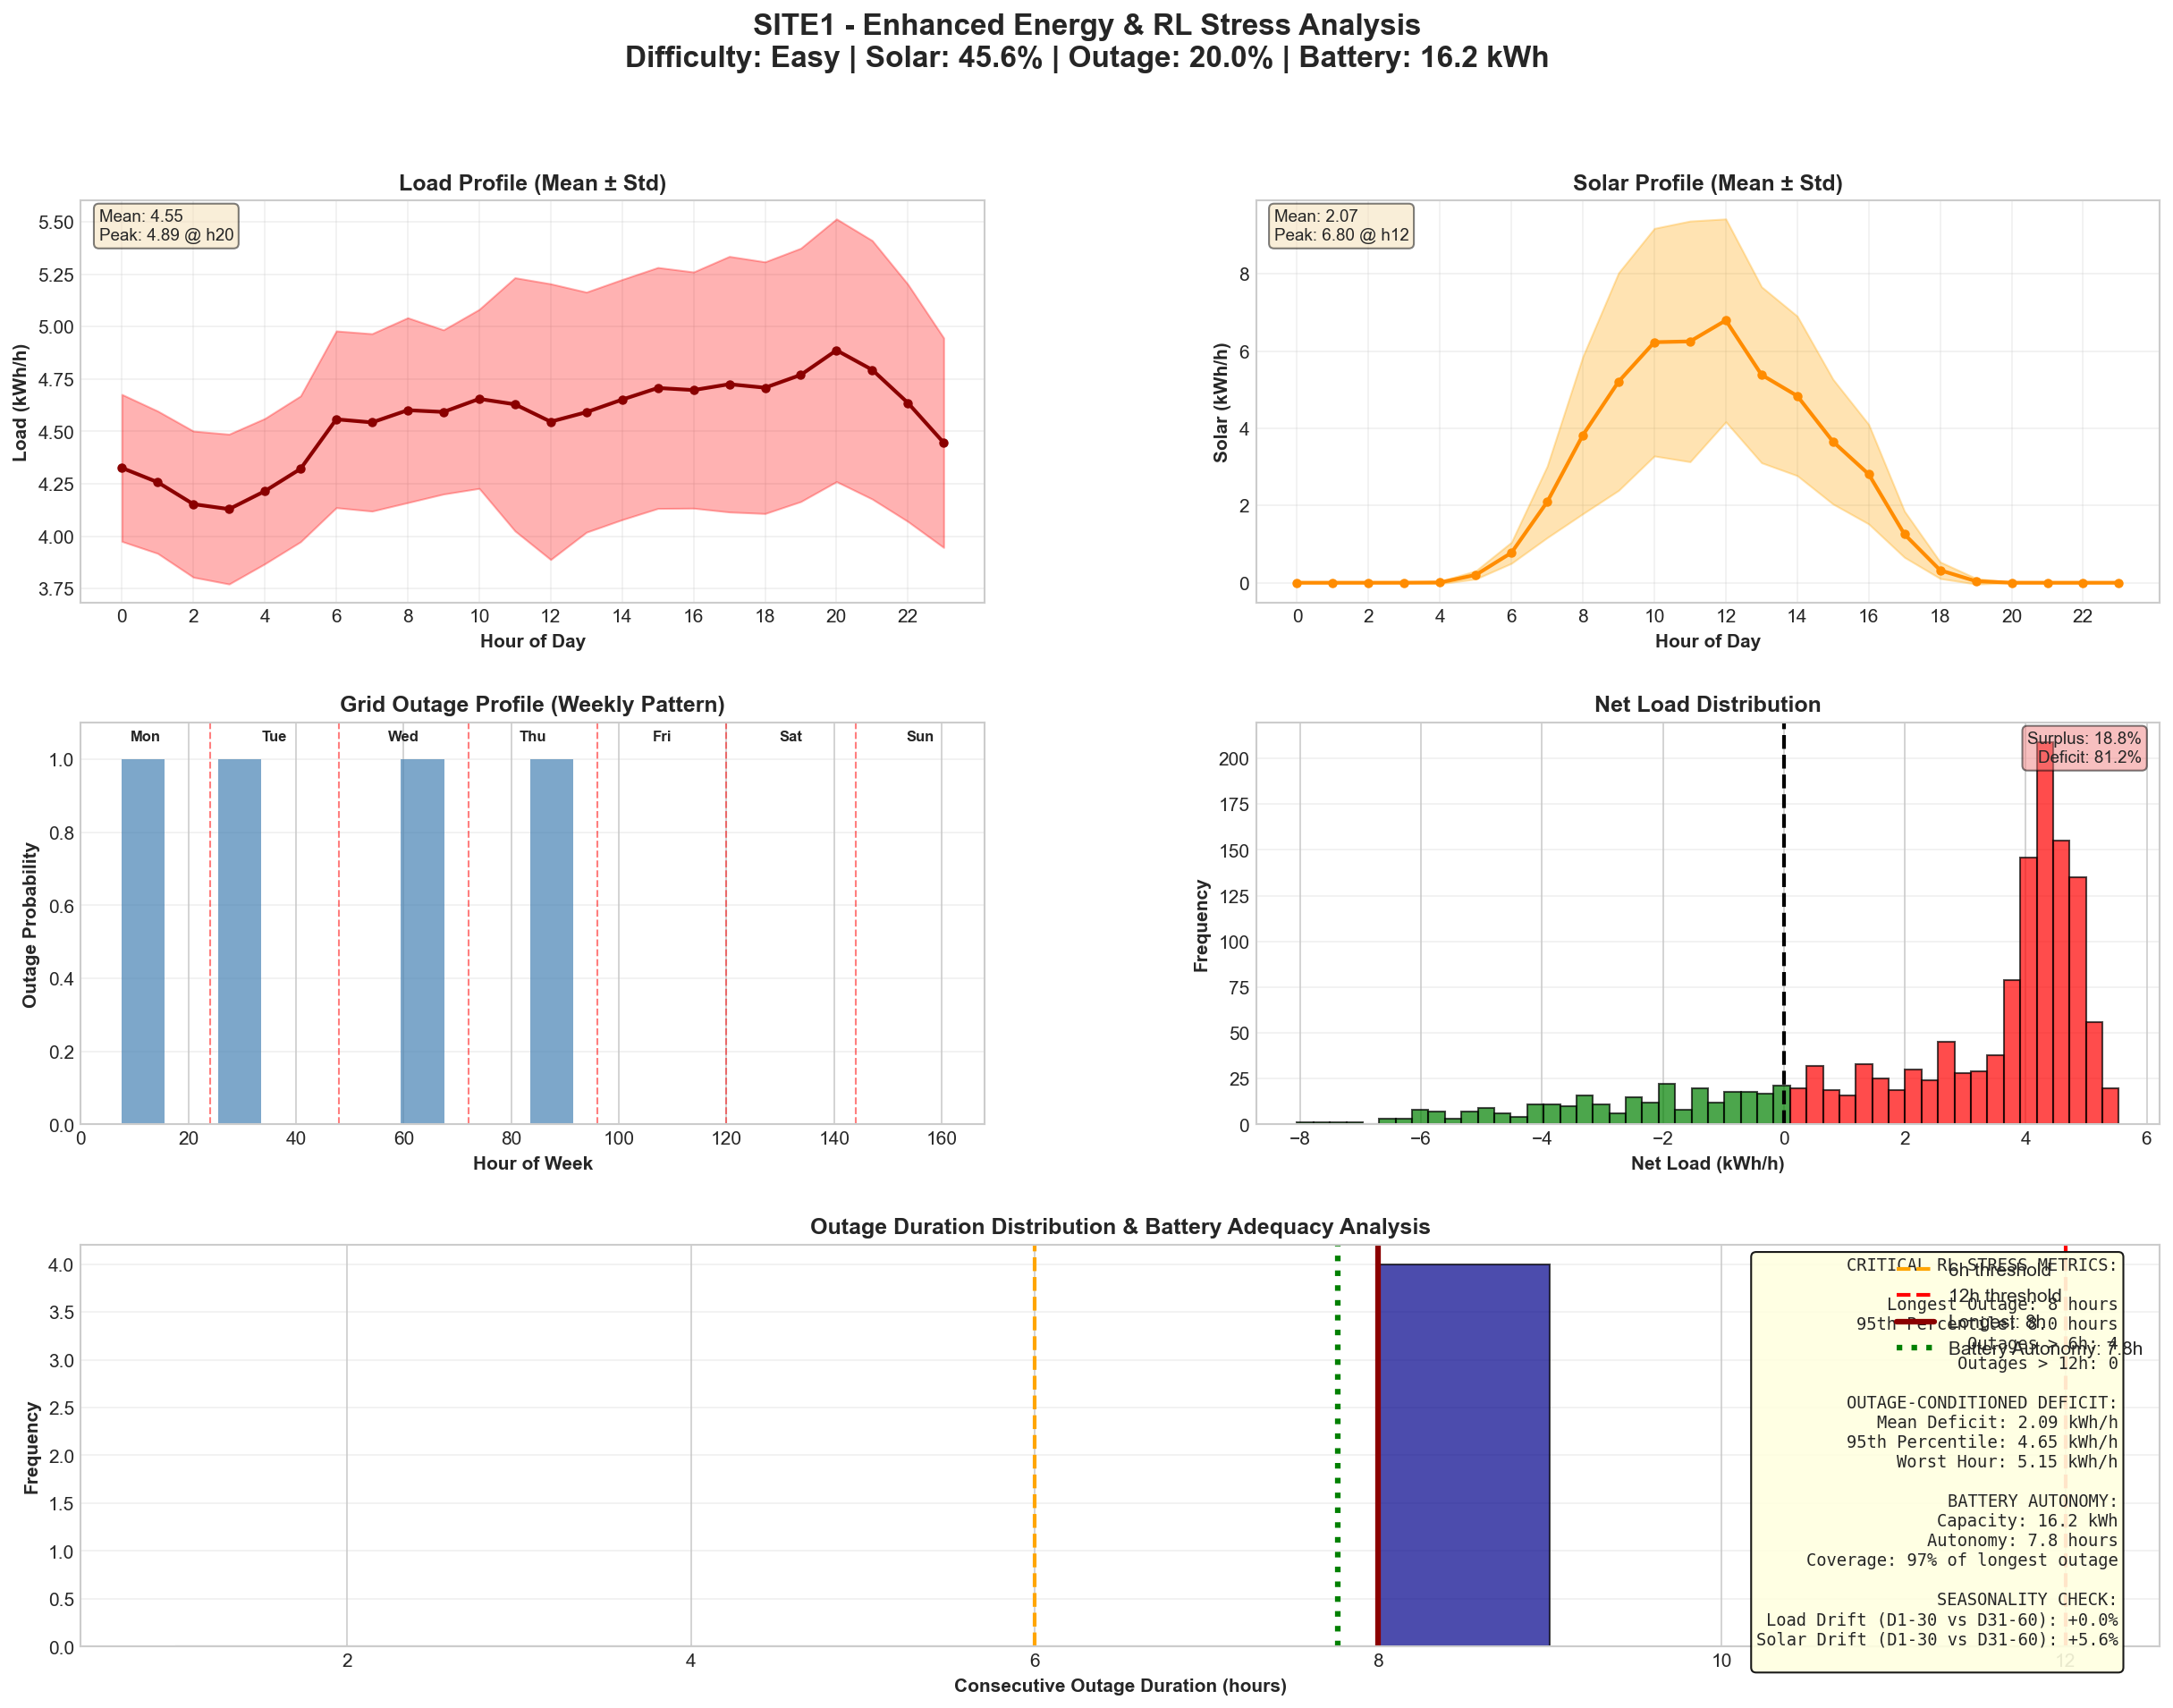
\includegraphics[width=\textwidth]{images/site1_enhanced_analysis}
\caption{Site~1 --- Easy. Load mean 4.55\,kWh/h; solar coverage 45.6\%;
grid availability 80.0\%; battery autonomy 7.8\,h (97\% of longest outage).
No outages exceed 12\,h. Outage-conditioned mean deficit 2.09\,kWh/h.}
\label{fig:app_site1}
\end{figure}

\begin{figure}[htbp]
\centering
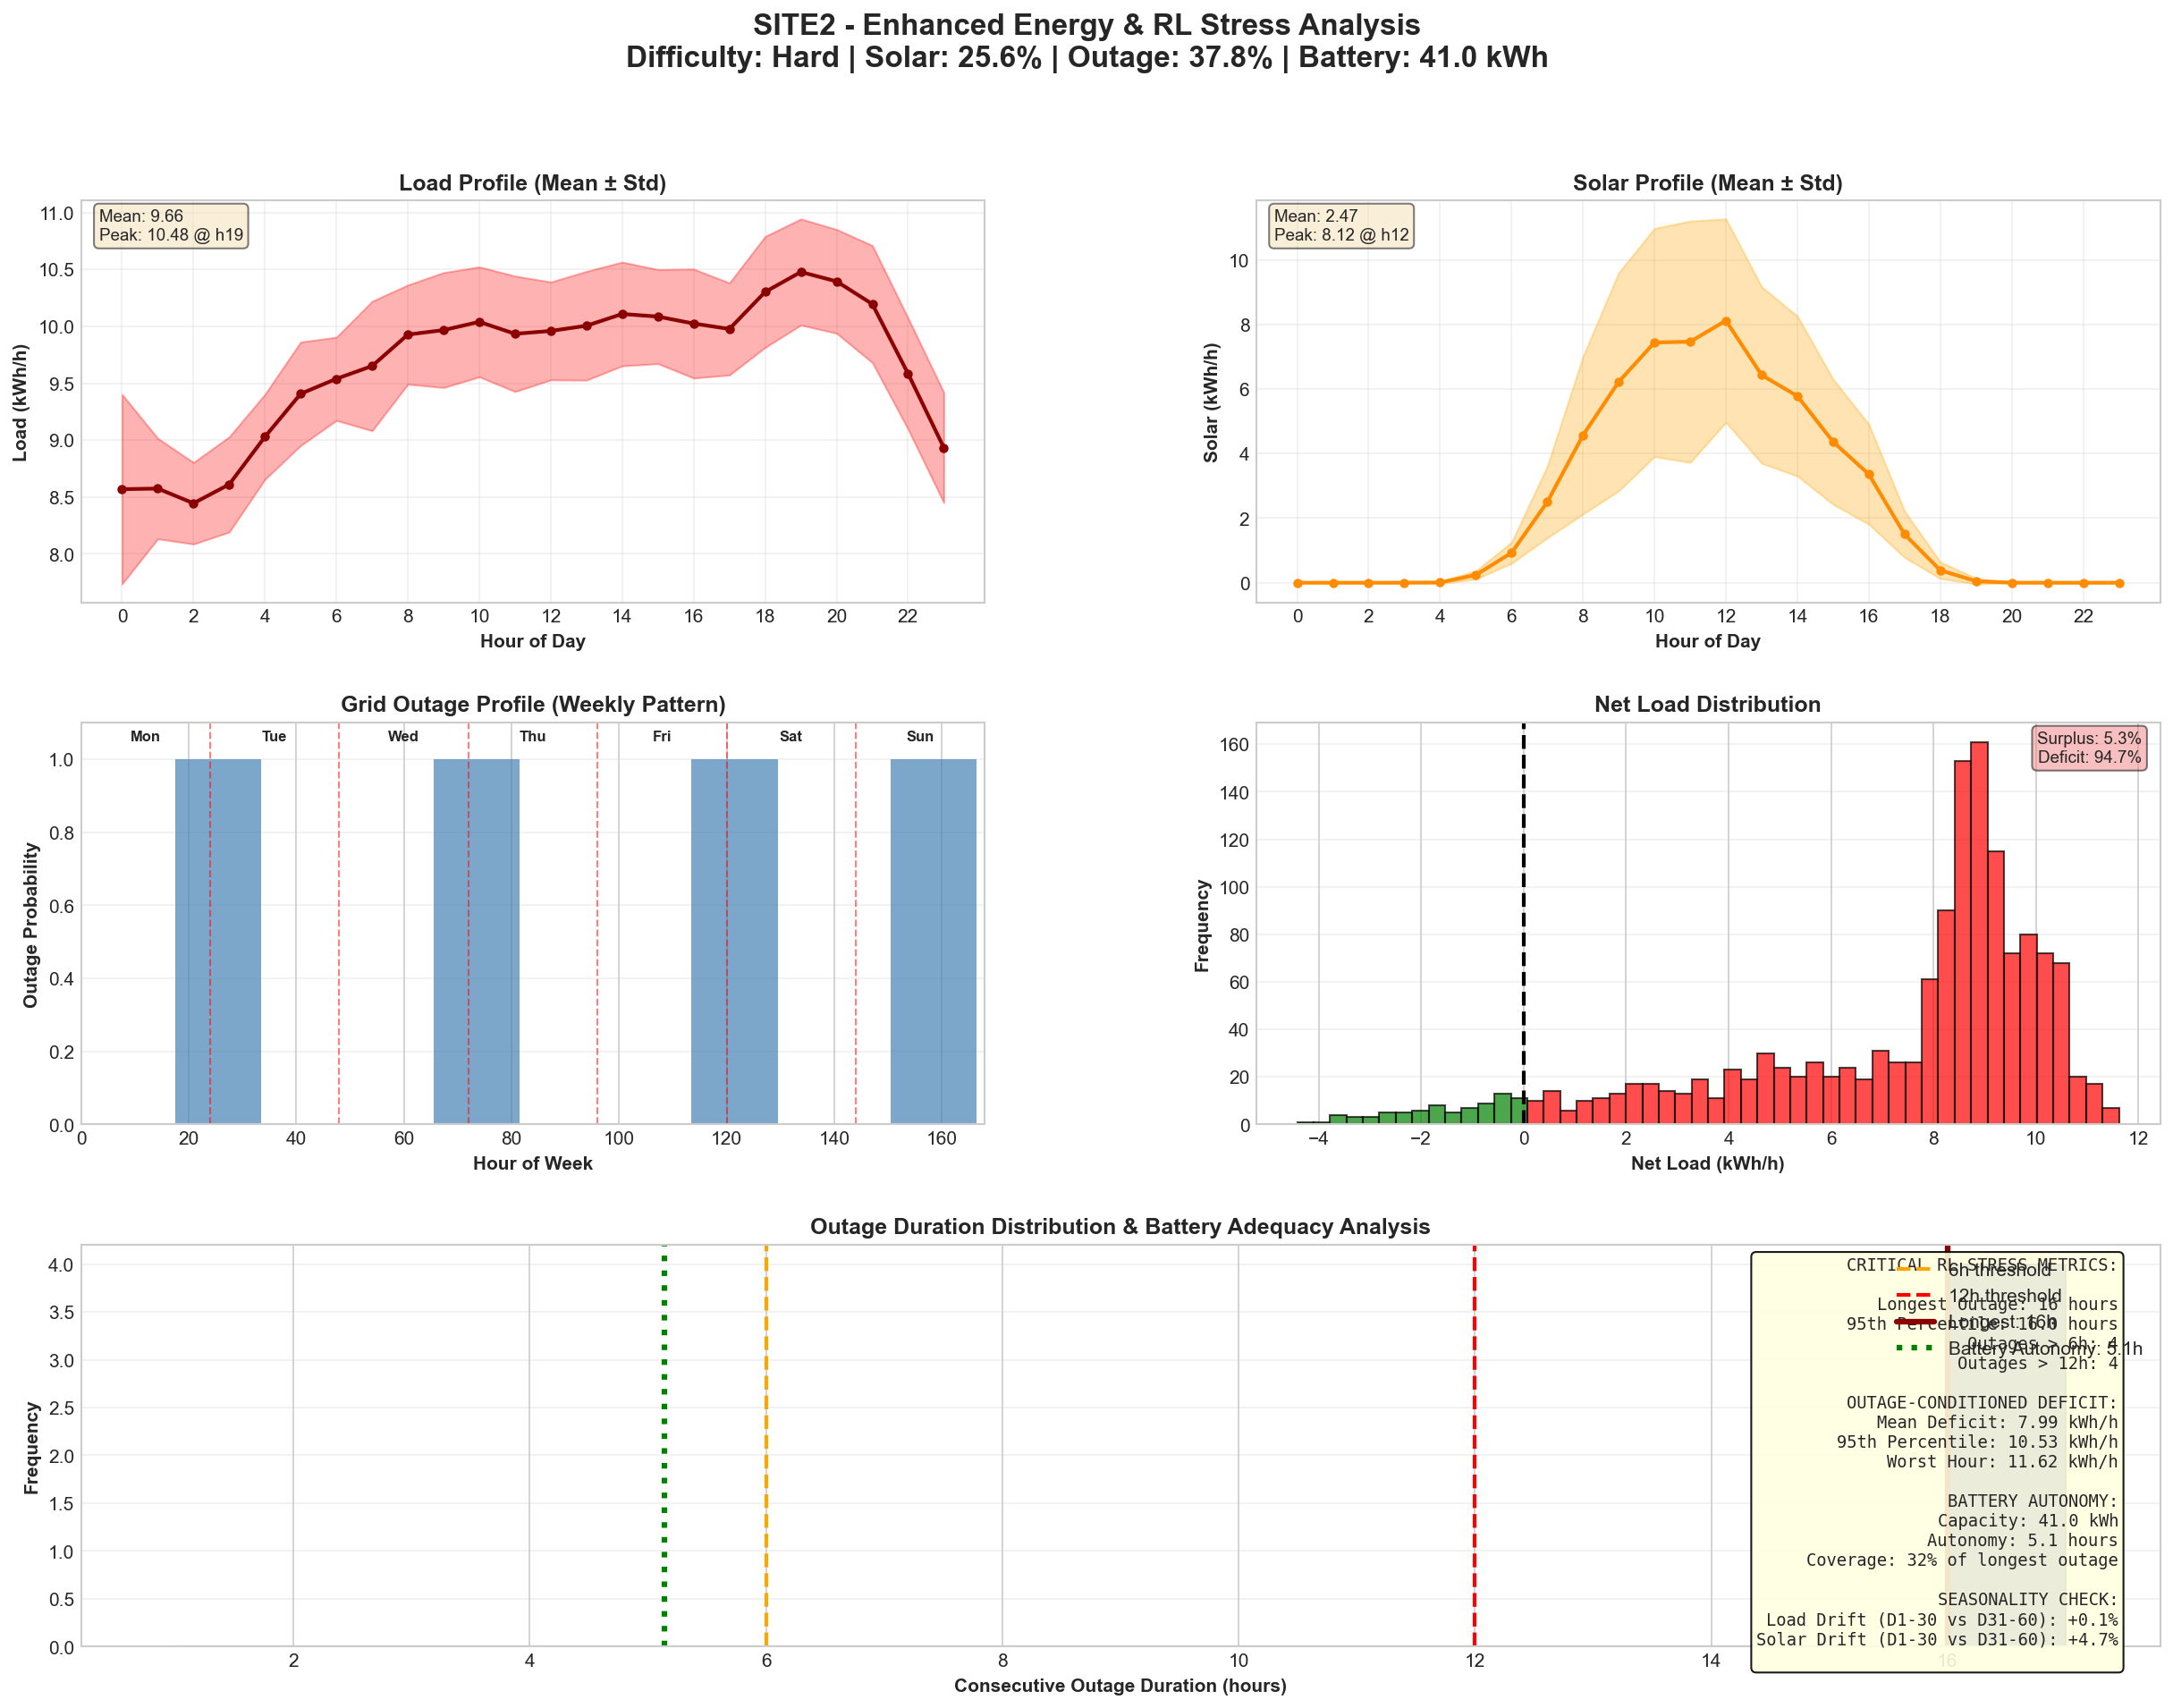
\includegraphics[width=\textwidth]{images/site2_enhanced_analysis}
\caption{Site~2 --- Hard. Load mean 9.66\,kWh/h (highest in dataset);
solar coverage 25.6\% (lowest); battery autonomy 5.1\,h (32\% of longest
outage). Four outages exceed 12\,h. Outage-conditioned mean deficit
7.99\,kWh/h.}
\label{fig:app_site2}
\end{figure}

\begin{figure}[htbp]
\centering
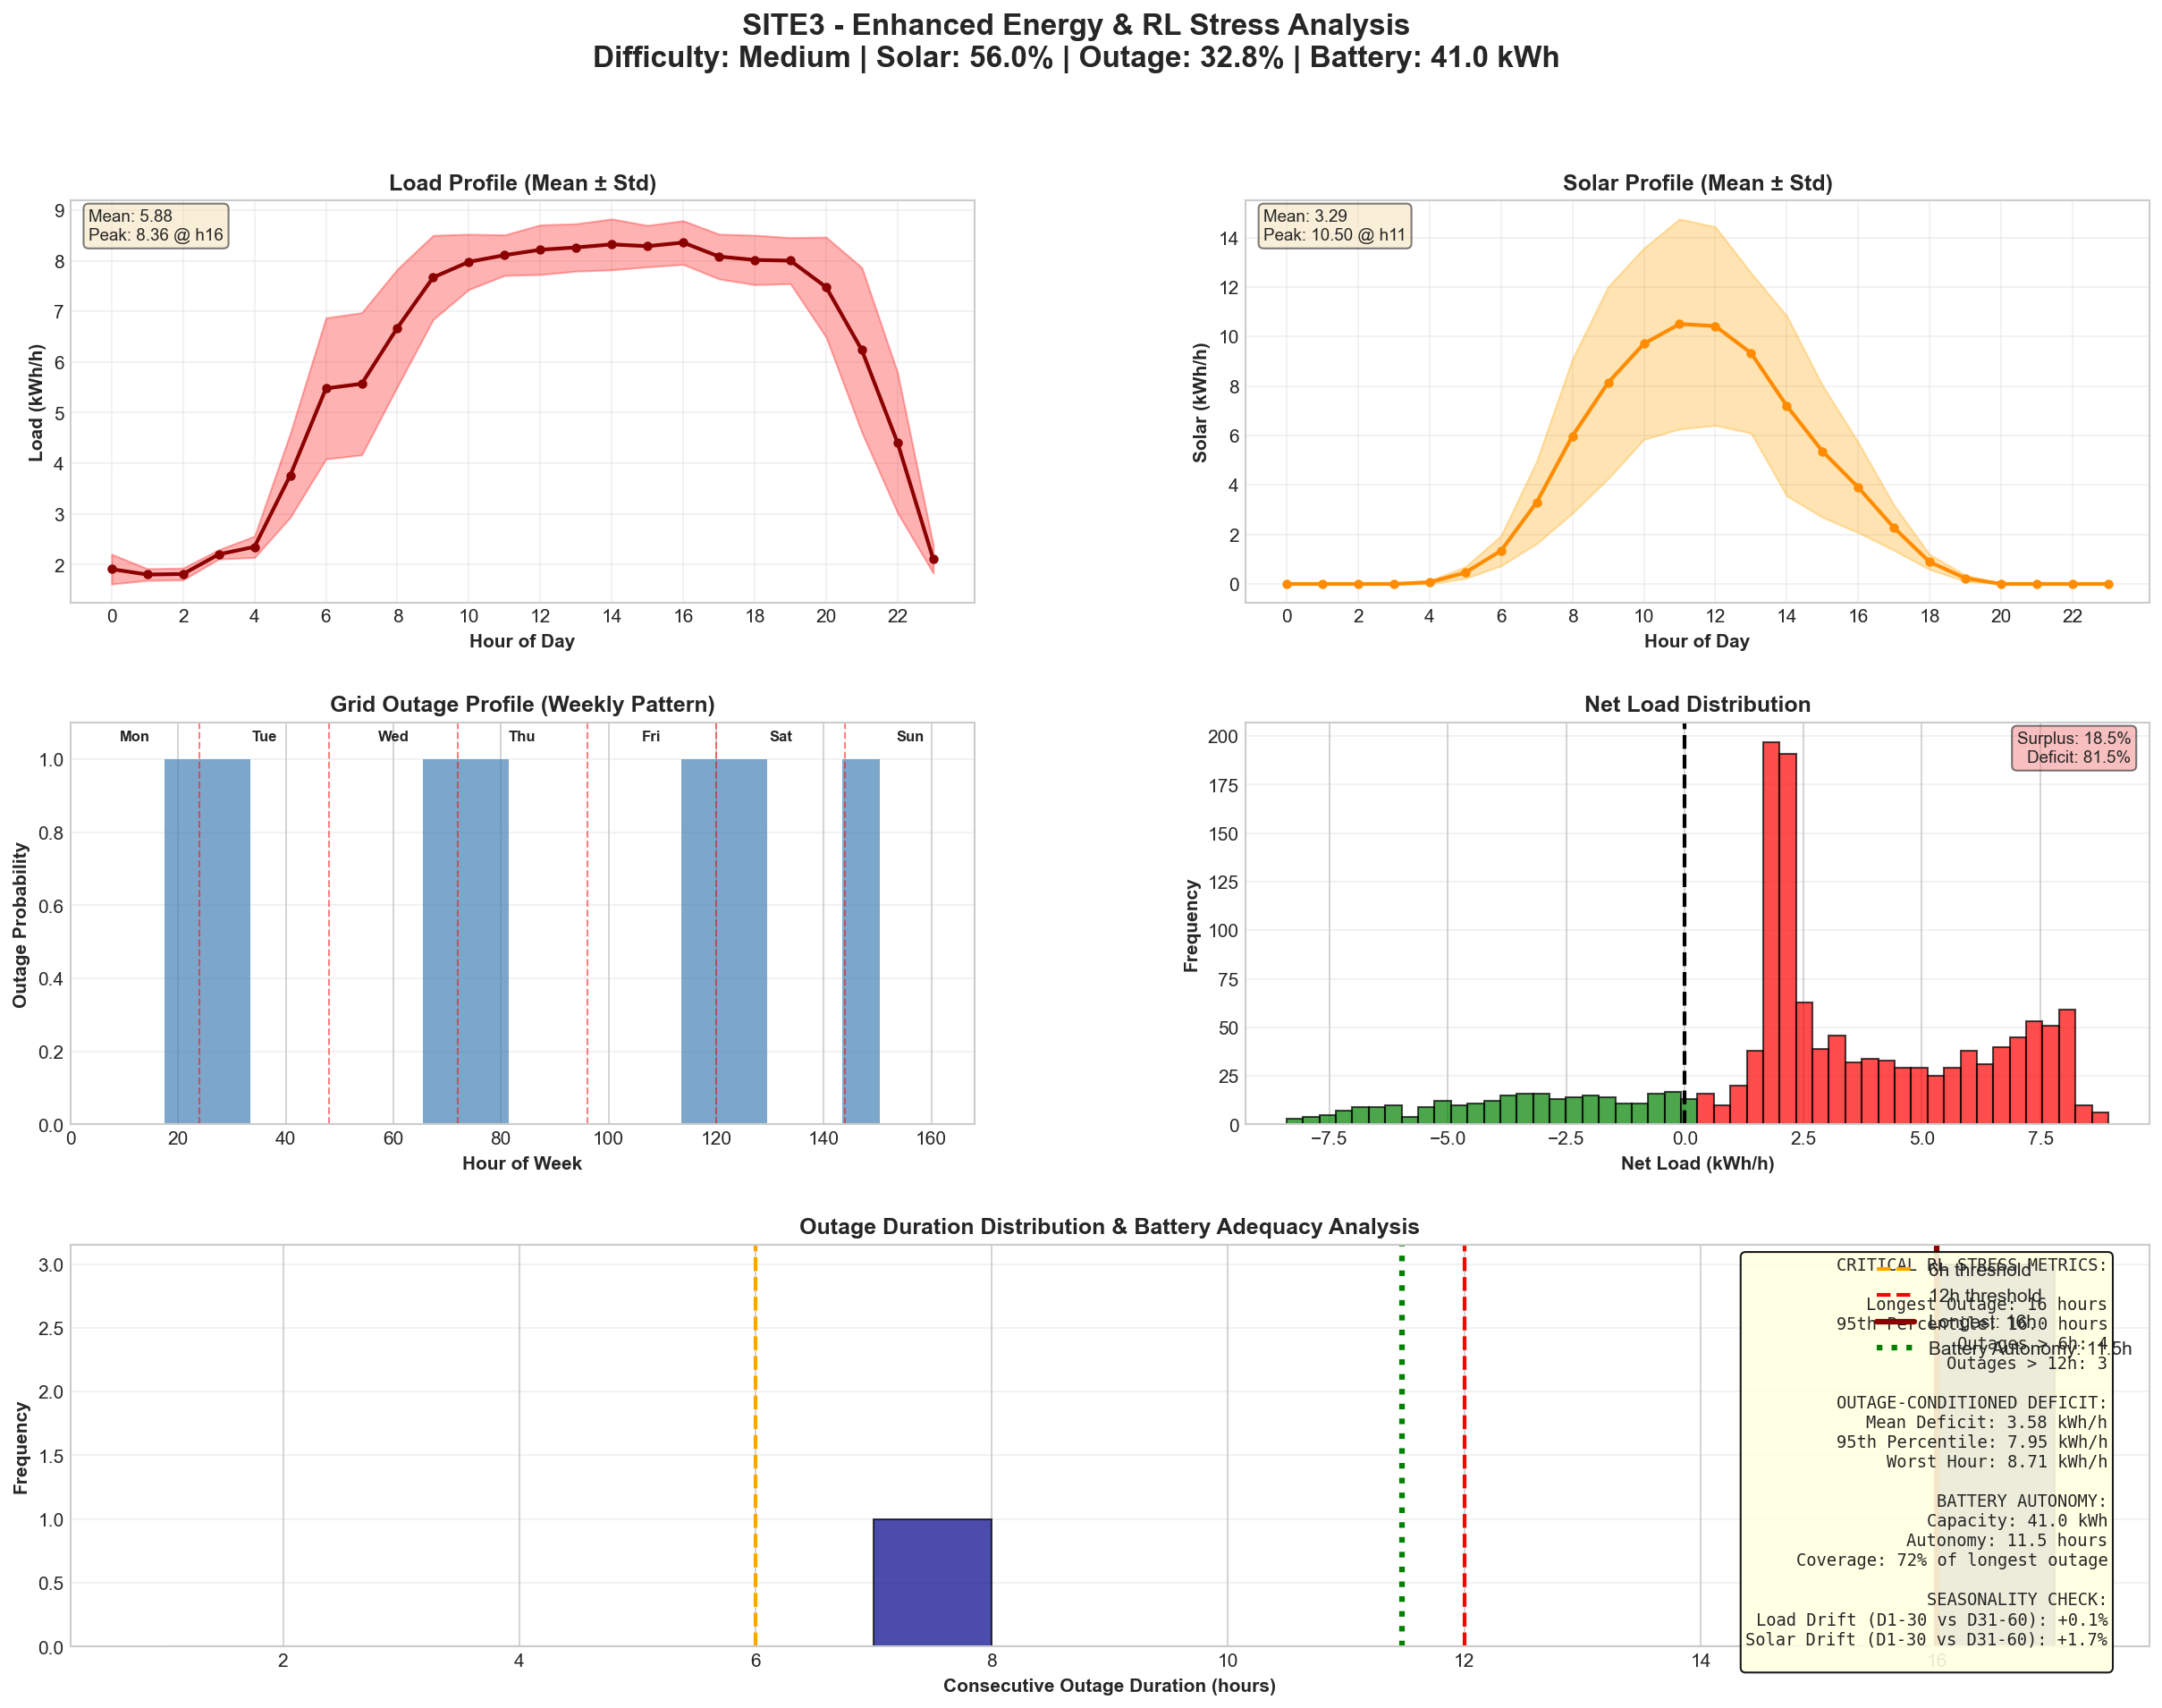
\includegraphics[width=\textwidth]{images/site3_enhanced_analysis}
\caption{Site~3 --- Medium. Load mean 5.88\,kWh/h; solar coverage 56.0\%;
battery autonomy 11.5\,h (72\% of longest outage). Three outages exceed
12\,h. Outage-conditioned mean deficit 3.58\,kWh/h.}
\label{fig:app_site3}
\end{figure}

\begin{figure}[htbp]
\centering
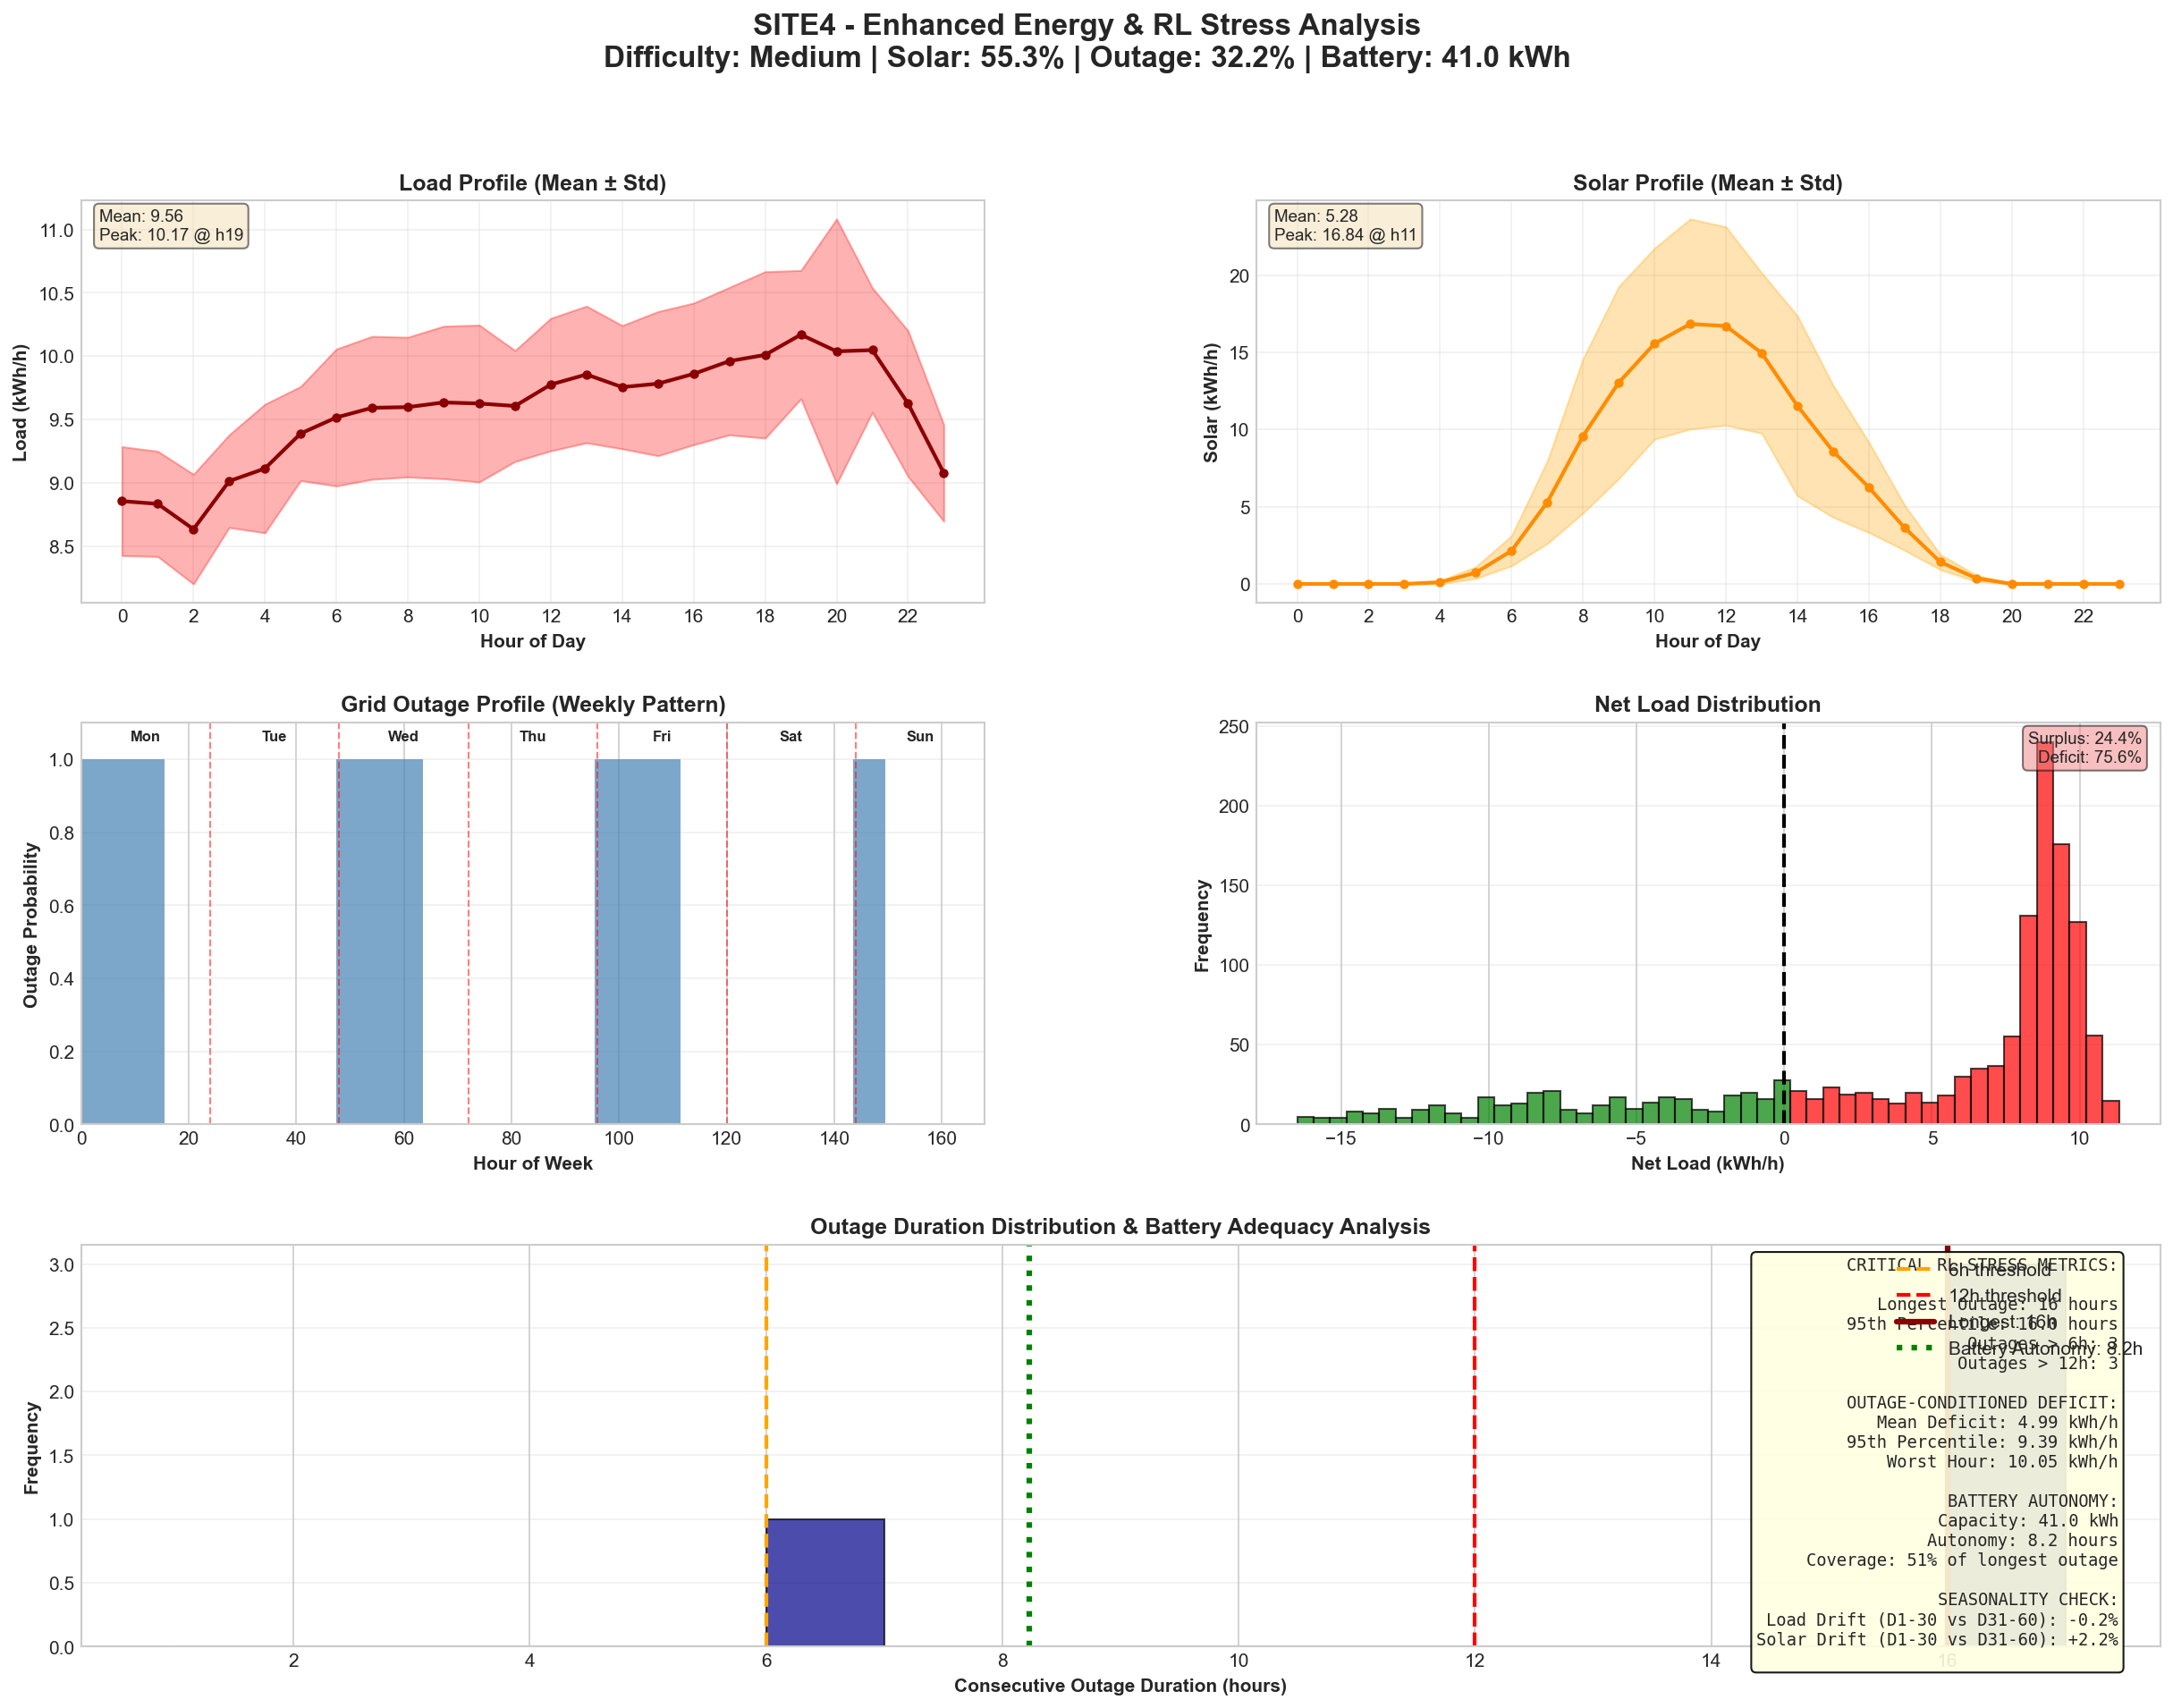
\includegraphics[width=\textwidth]{images/site4_enhanced_analysis}
\caption{Site~4 --- Medium. Load mean 9.56\,kWh/h; solar coverage 55.3\%;
battery autonomy 8.2\,h (51\% of longest outage). Three outages exceed
12\,h. Outage-conditioned mean deficit 4.99\,kWh/h. Notable for
combining high load with reasonable solar coverage.}
\label{fig:app_site4}
\end{figure}

\begin{figure}[htbp]
\centering
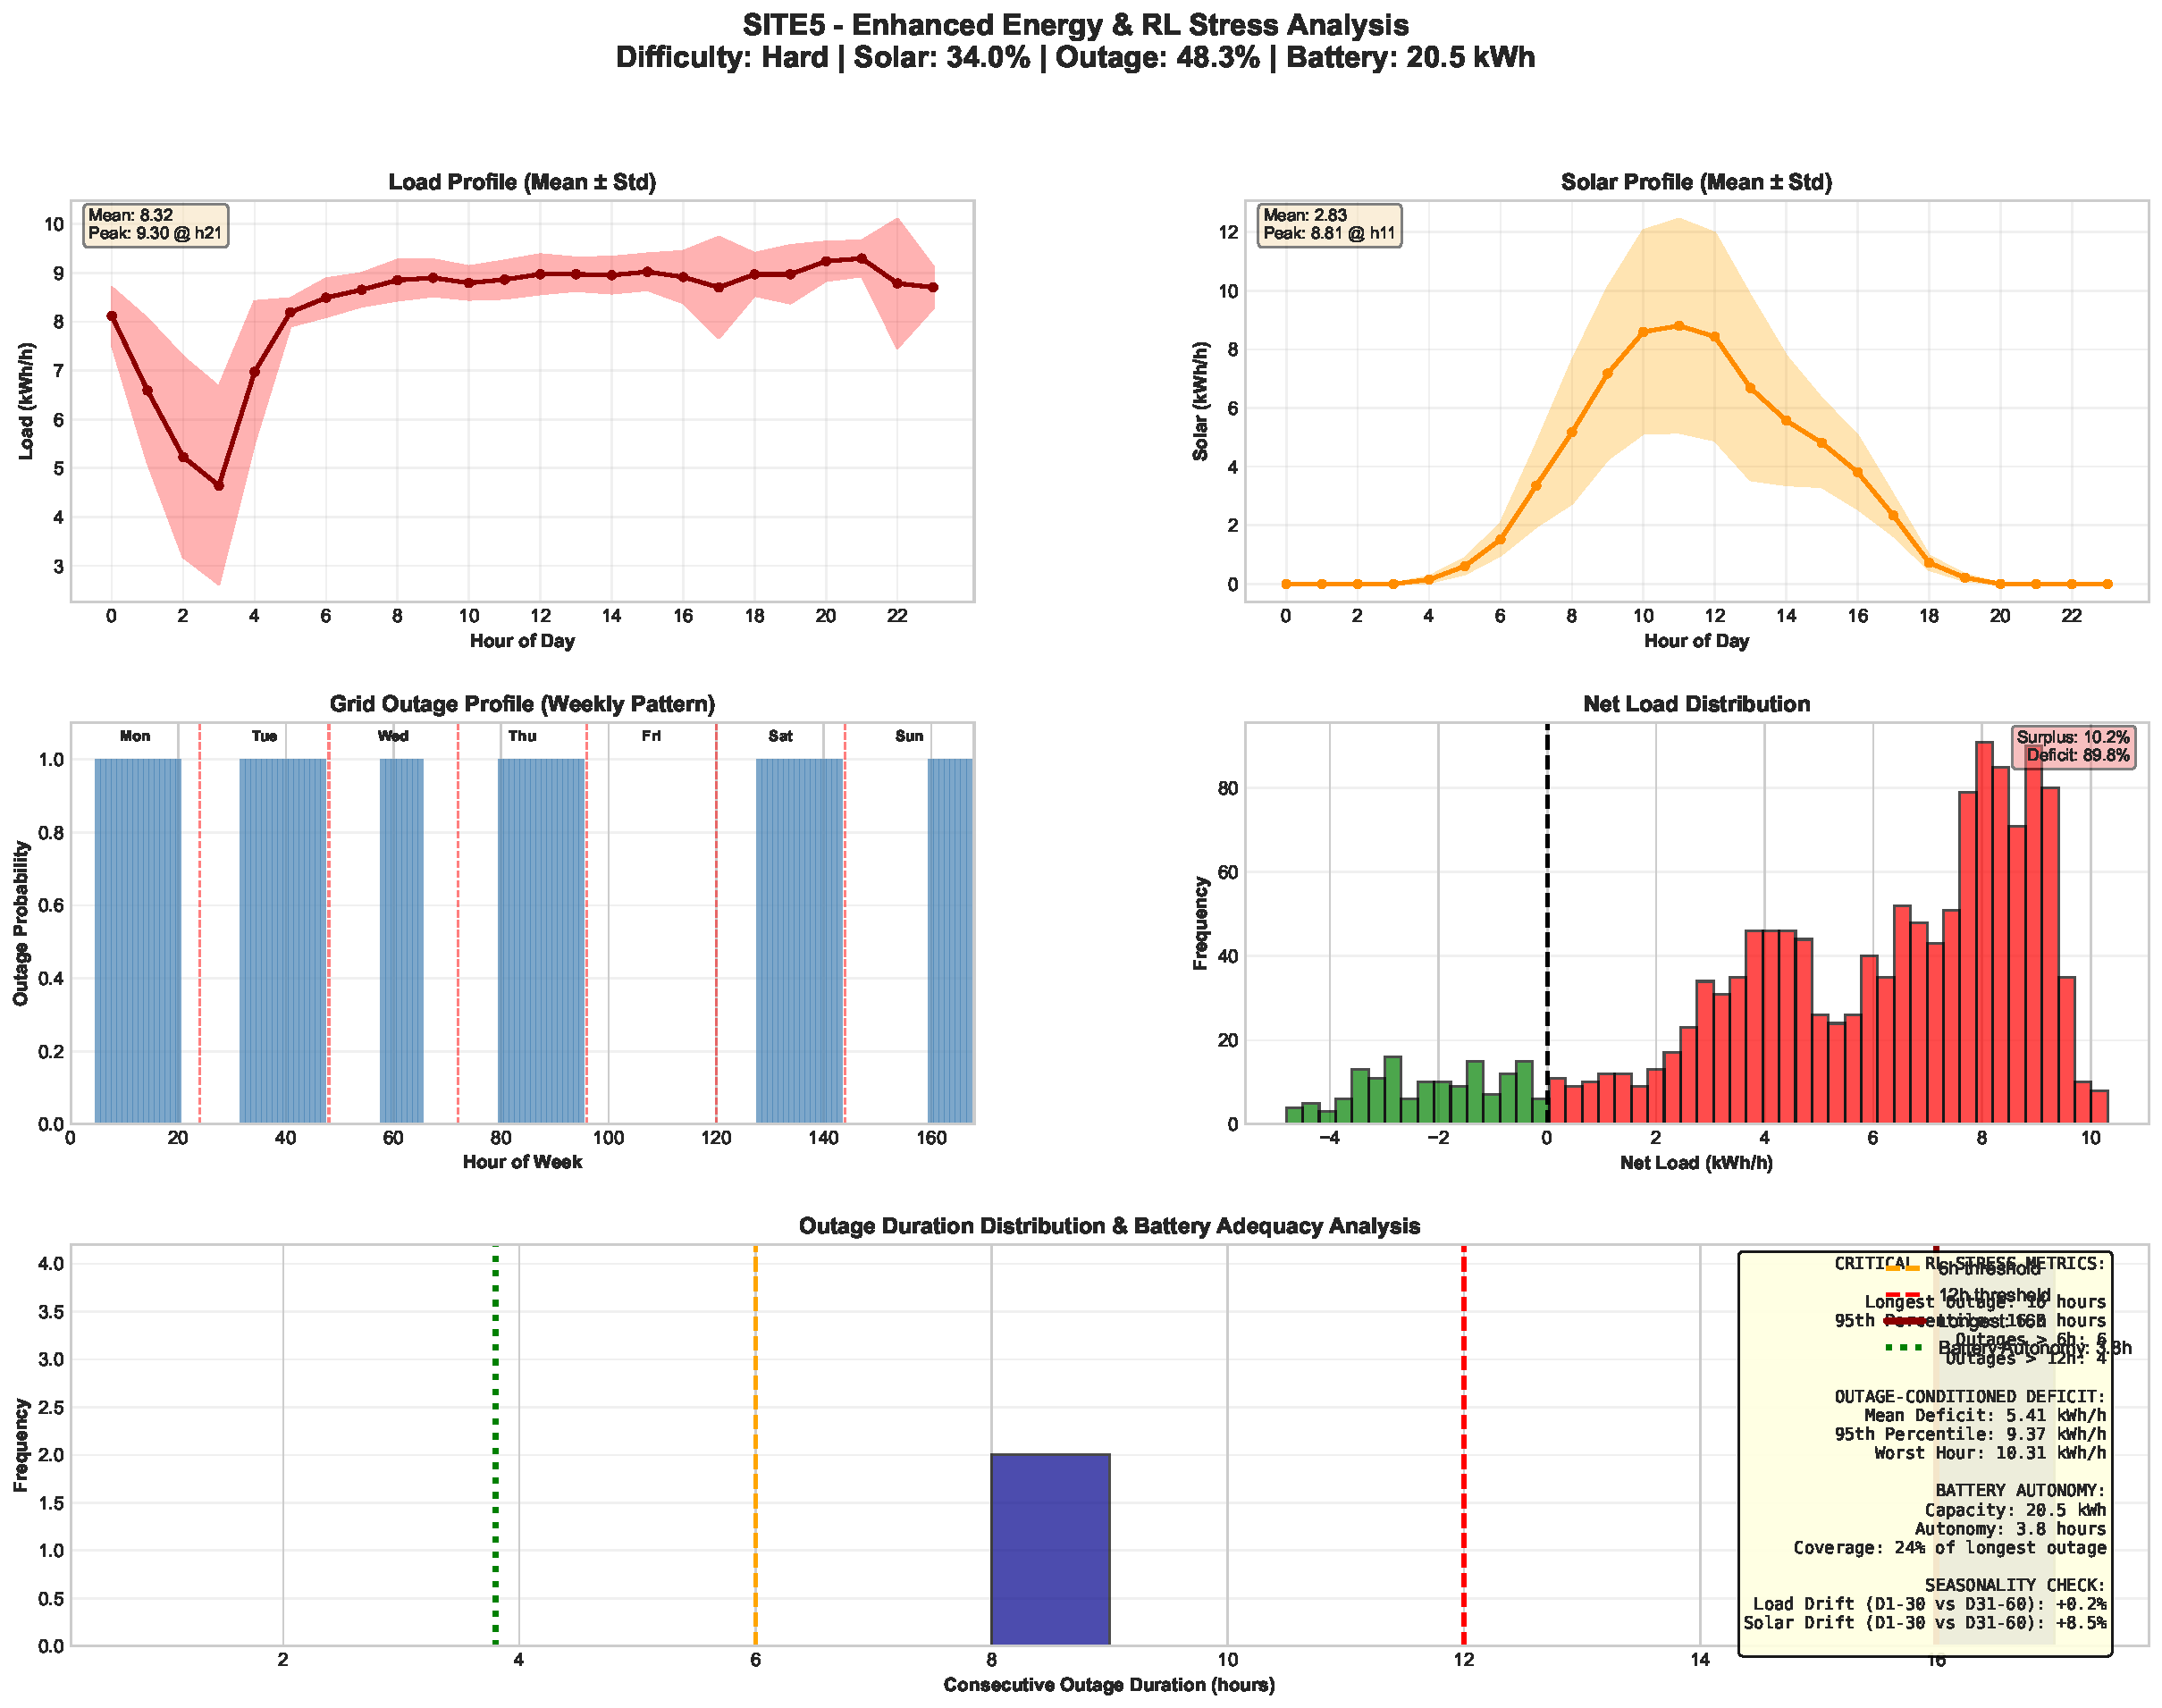
\includegraphics[width=\textwidth]{images/site5_enhanced_analysis}
\caption{Site~5 --- Hard. Load mean 8.32\,kWh/h; solar coverage 34.0\%;
battery autonomy 3.8\,h (24\% of longest outage). 52 outage events ---
highest frequency in dataset. Four outages exceed 12\,h.
Outage-conditioned mean deficit 5.41\,kWh/h.}
\label{fig:app_site5}
\end{figure}

\begin{figure}[htbp]
\centering
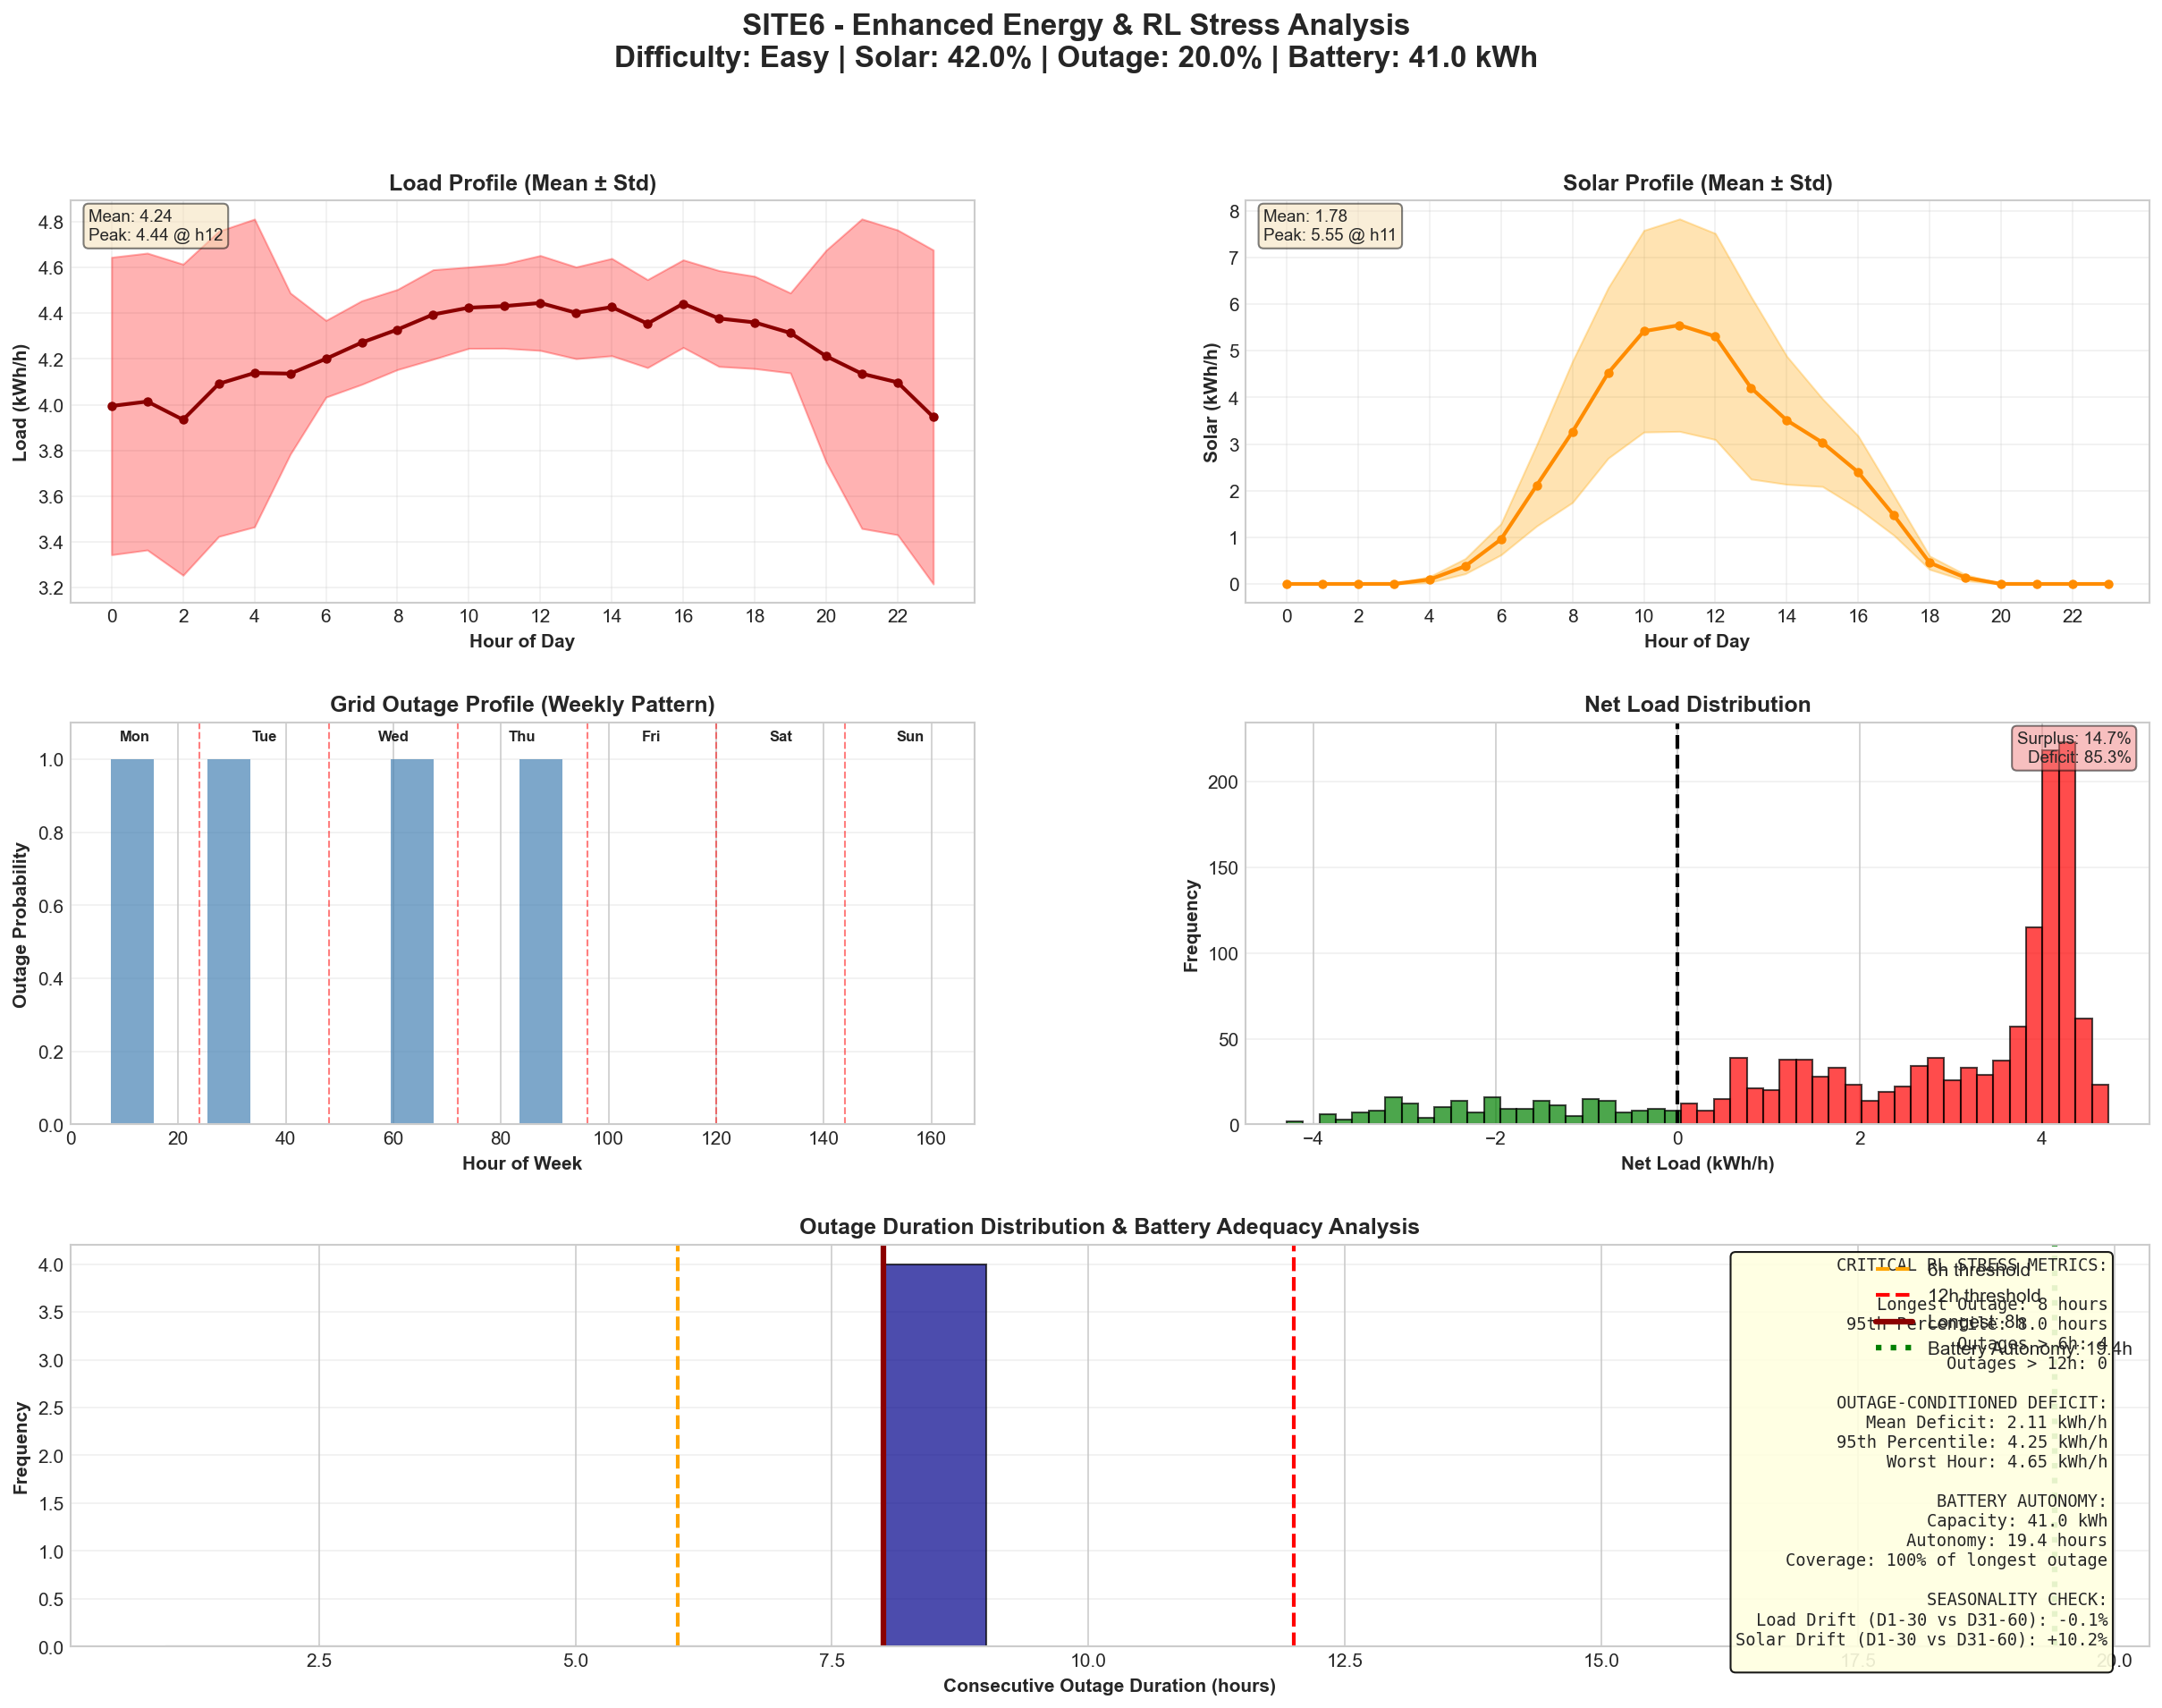
\includegraphics[width=\textwidth]{images/site6_enhanced_analysis}
\caption{Site~6 --- Easy. Load mean 4.24\,kWh/h; solar coverage 42.0\%;
grid availability 80.0\%; battery autonomy 19.4\,h (100\% of longest
outage). No outages exceed 12\,h. Outage-conditioned mean deficit
2.11\,kWh/h. Site~6 is the most battery-adequate site in the dataset.}
\label{fig:app_site6}
\end{figure}

\begin{figure}[htbp]
\centering
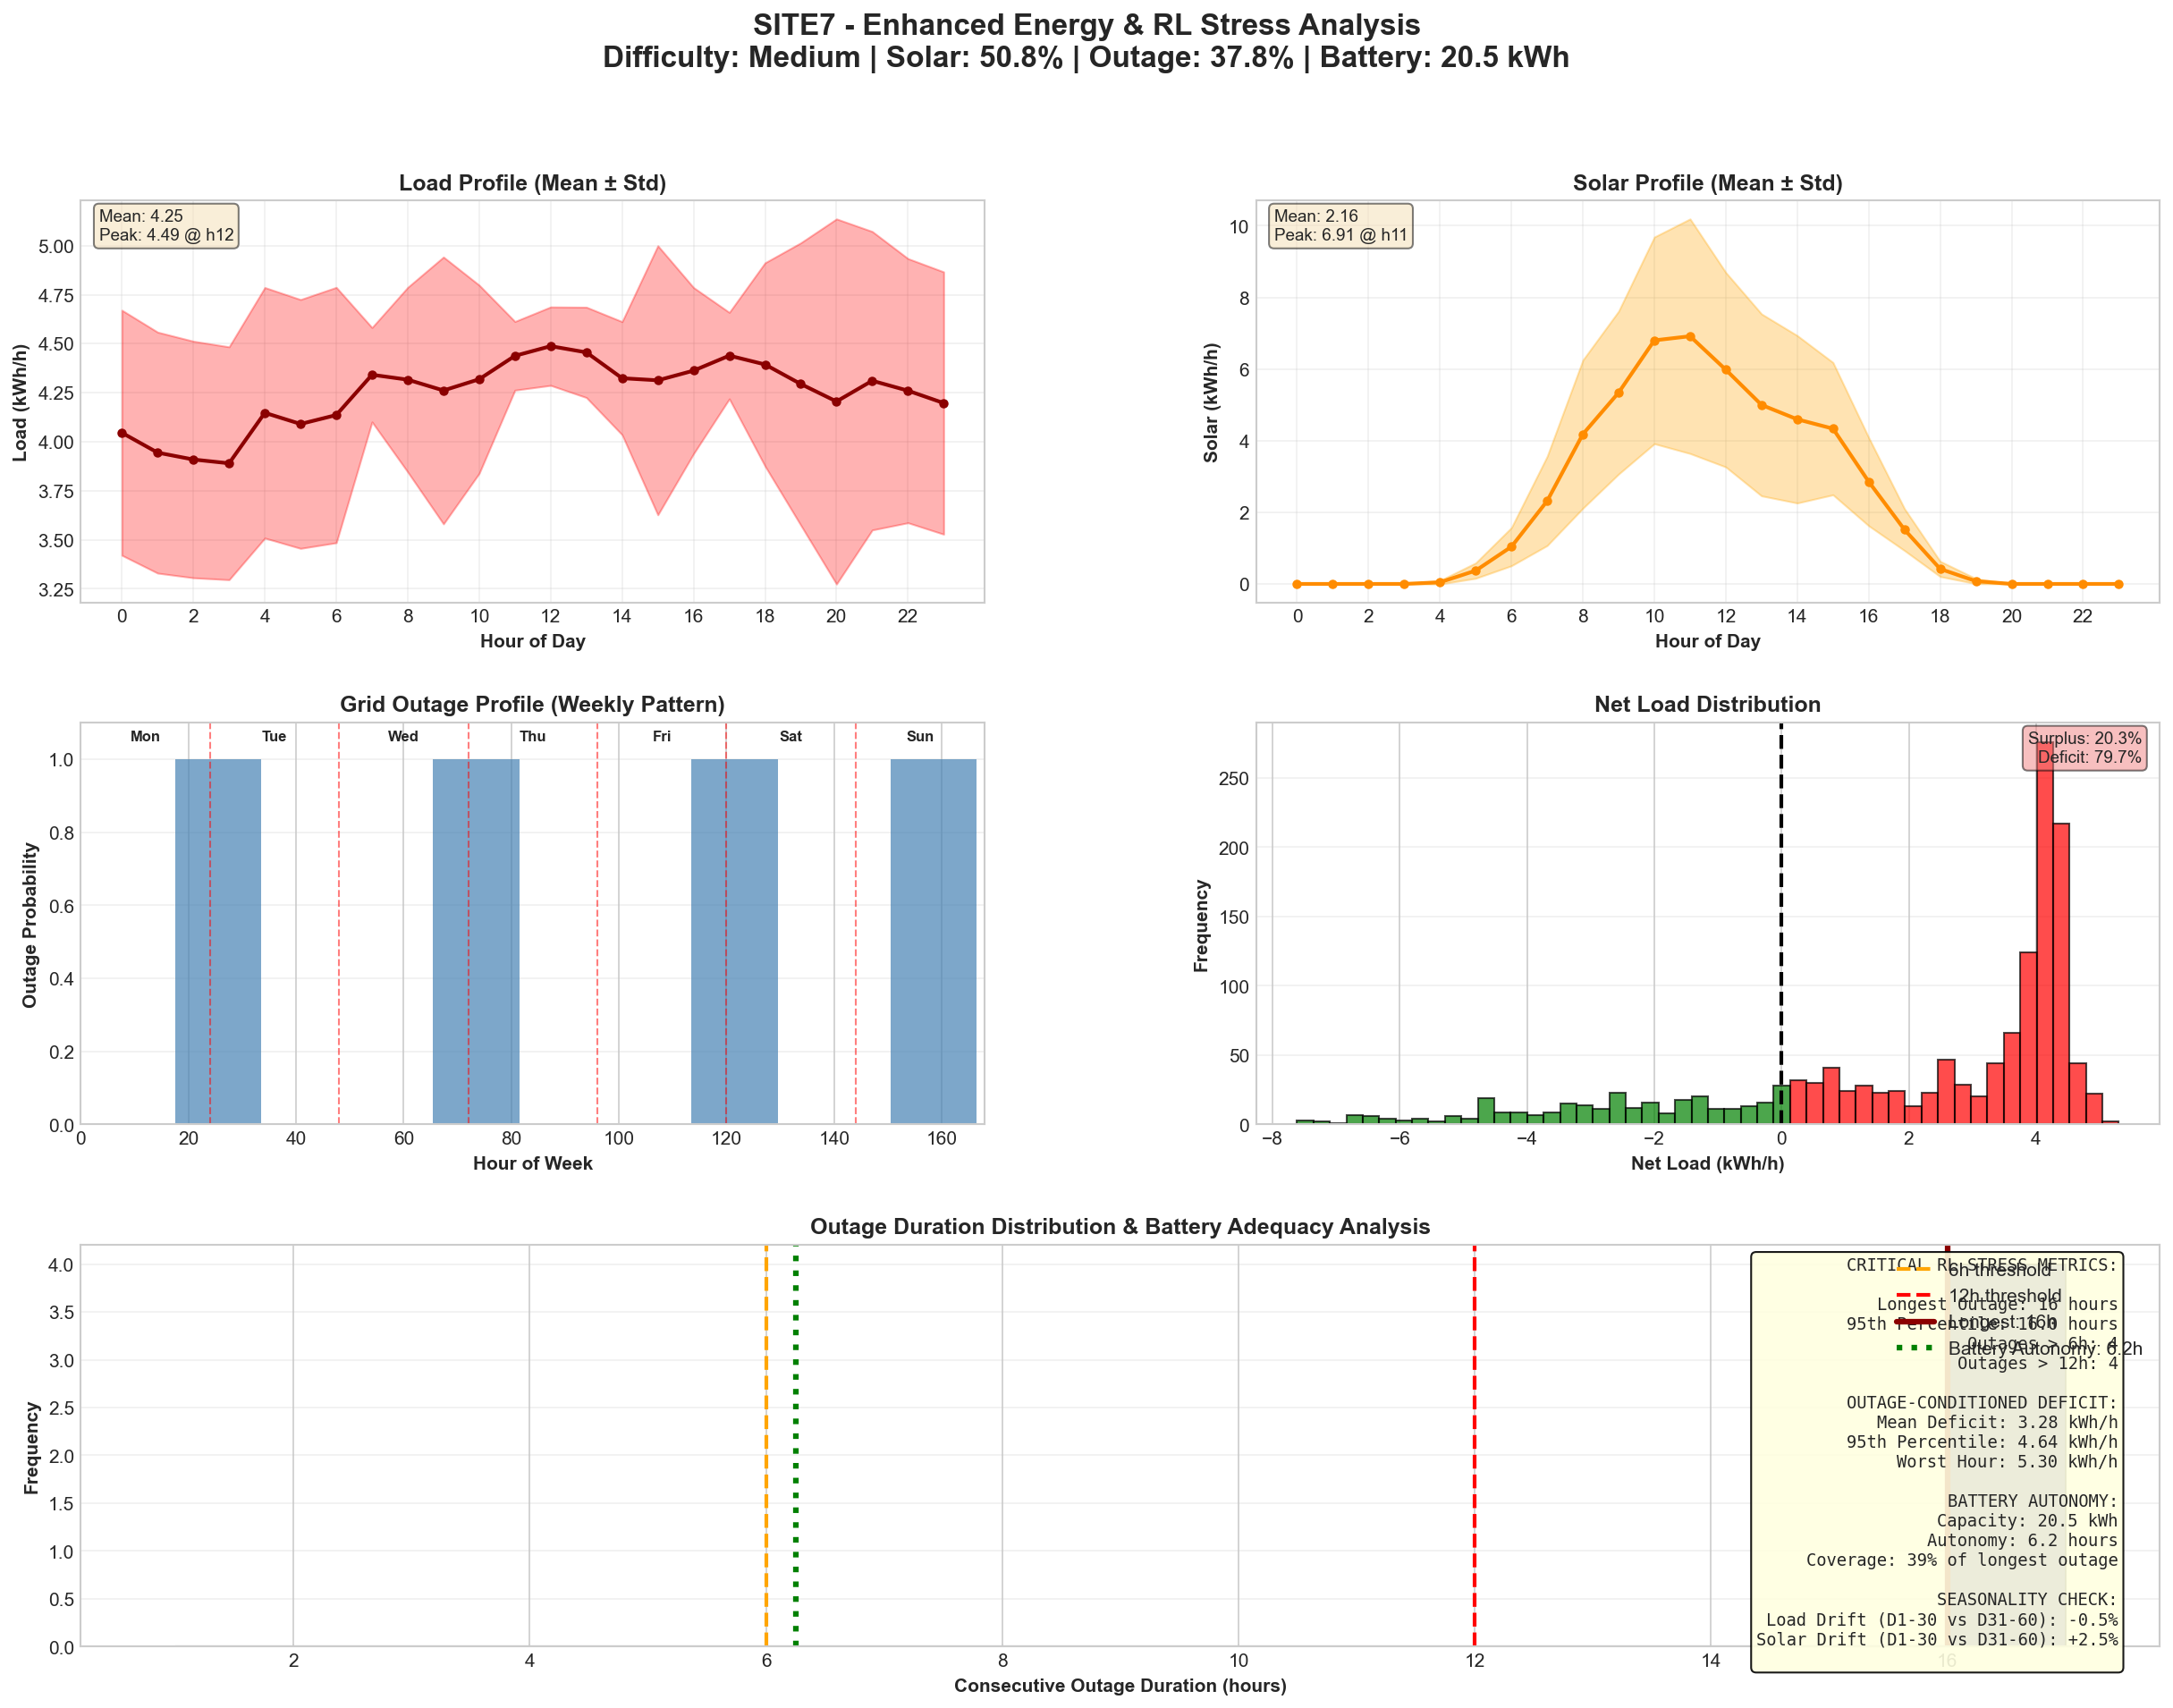
\includegraphics[width=\textwidth]{images/site7_enhanced_analysis}
\caption{Site~7 --- Medium. Load mean 4.25\,kWh/h; solar coverage 50.8\%;
battery autonomy 6.2\,h (39\% of longest outage). Four outages exceed
12\,h. Outage-conditioned mean deficit 3.28\,kWh/h. Despite moderate
load, battery undersizing relative to 16-hour outages creates reliability
risk.}
\label{fig:app_site7}
\end{figure}

\begin{figure}[htbp]
\centering
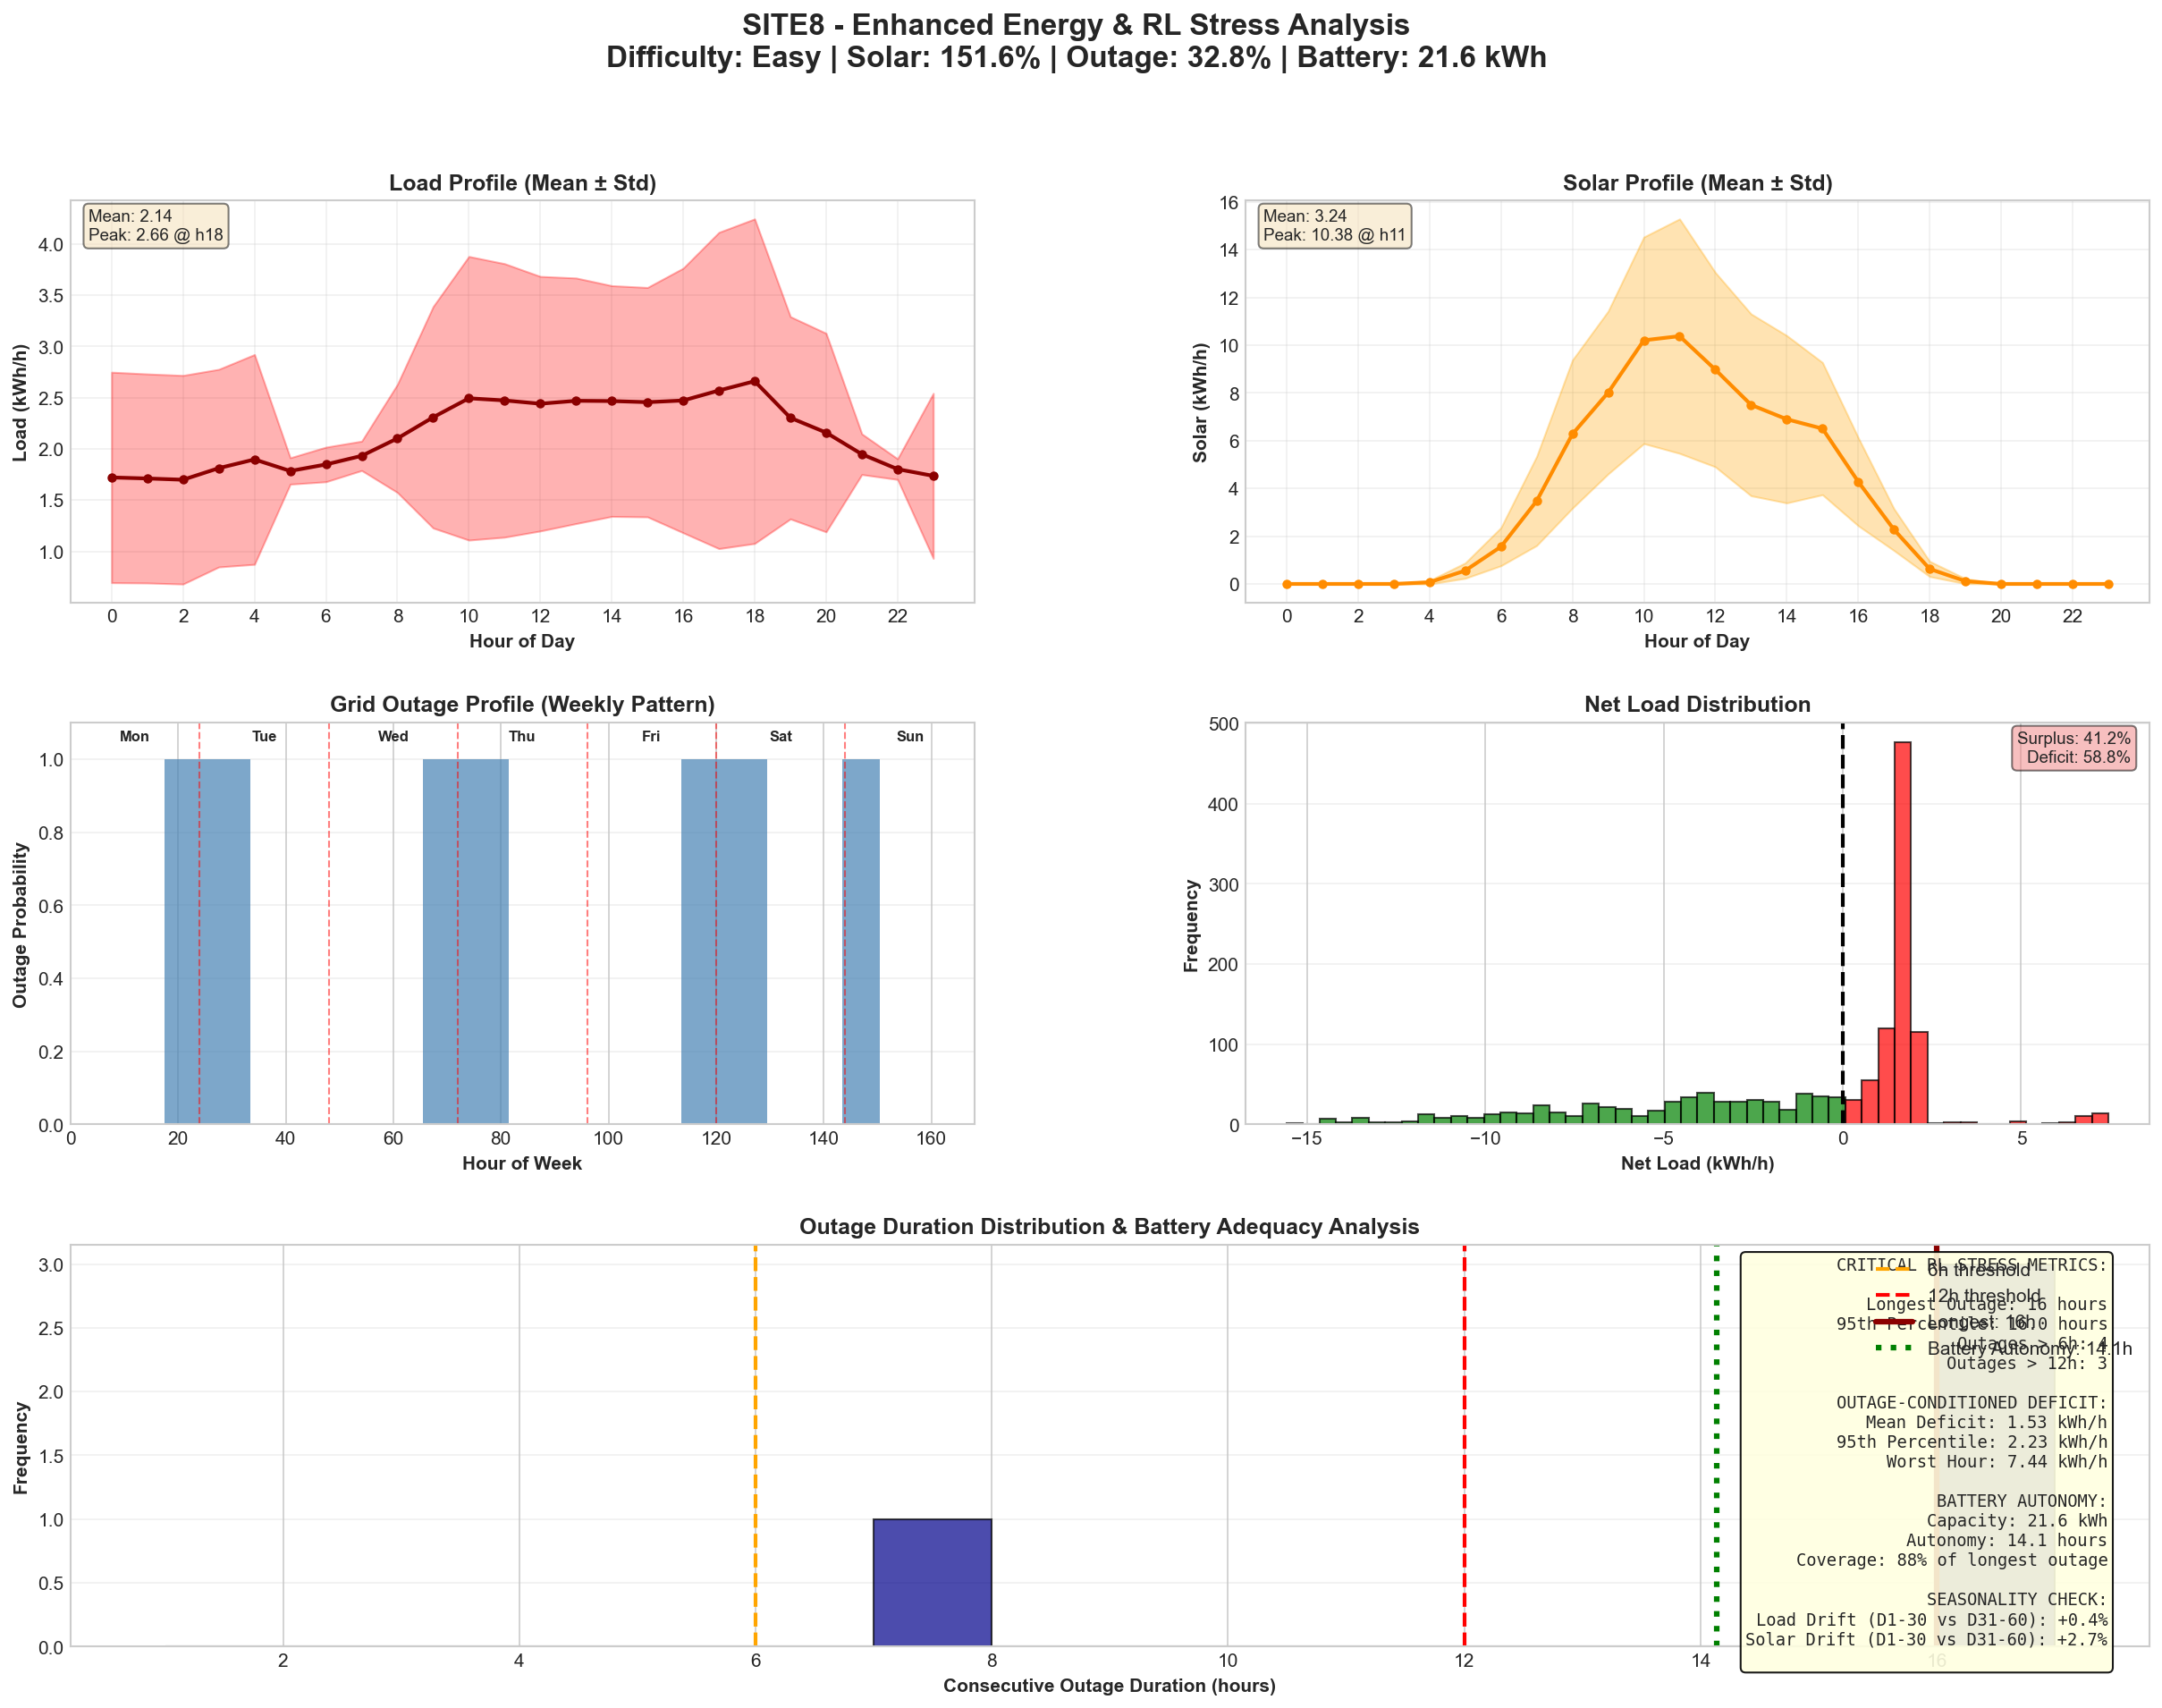
\includegraphics[width=\textwidth]{images/site8_enhanced_analysis}
\caption{Site~8 --- Easy (solar surplus). Load mean 2.14\,kWh/h; solar
coverage 151.6\%; battery autonomy 14.1\,h (88\% of longest outage).
41.2\% of hours are solar-surplus. Three outages exceed 12\,h but
outage-conditioned mean deficit is only 1.53\,kWh/h. Primary challenge
is battery saturation and curtailment, not stockout.}
\label{fig:app_site8}
\end{figure}

\begin{figure}[htbp]
\centering
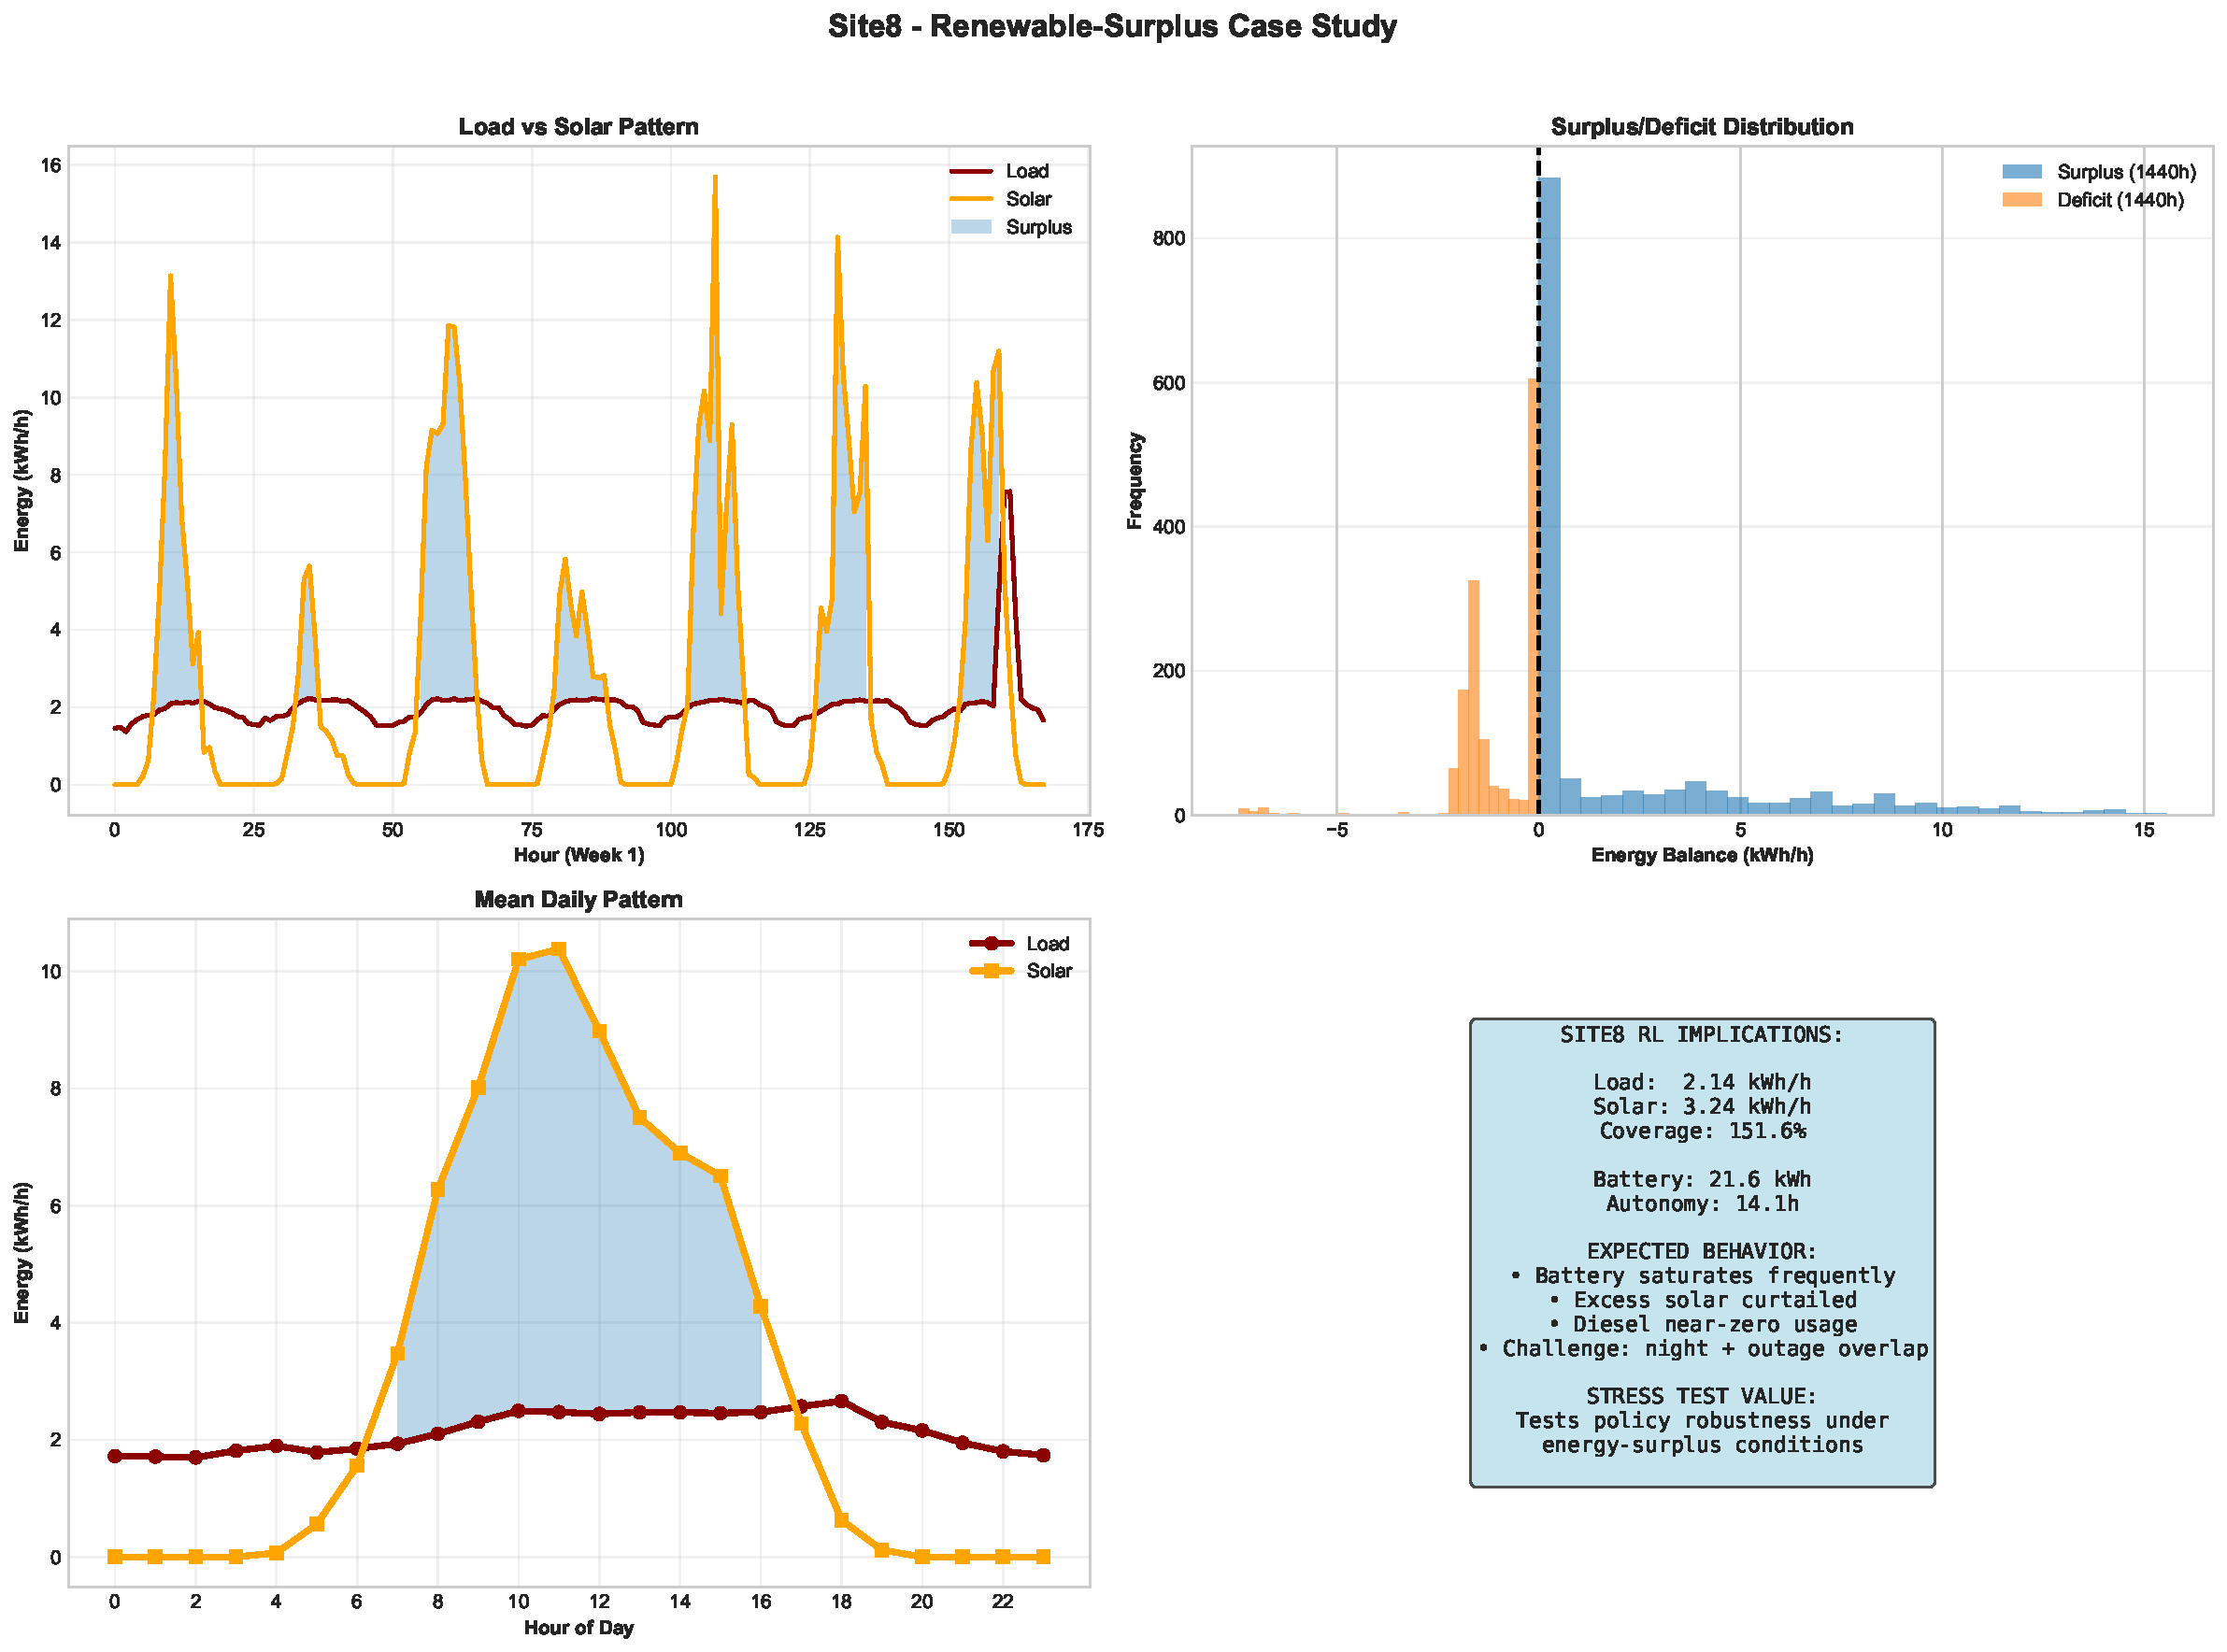
\includegraphics[width=\textwidth]{images/fig3_site8_surplus}
\caption{Site~8 renewable-surplus case study showing load vs.\ solar time
series (top-left), surplus/deficit distribution (top-right), and mean
daily pattern (bottom-left). 41\% of hours are solar-surplus; average
surplus 51\,kWh/day.}
\label{fig:app_site8_surplus}
\end{figure}

\begin{figure}[htbp]
\centering
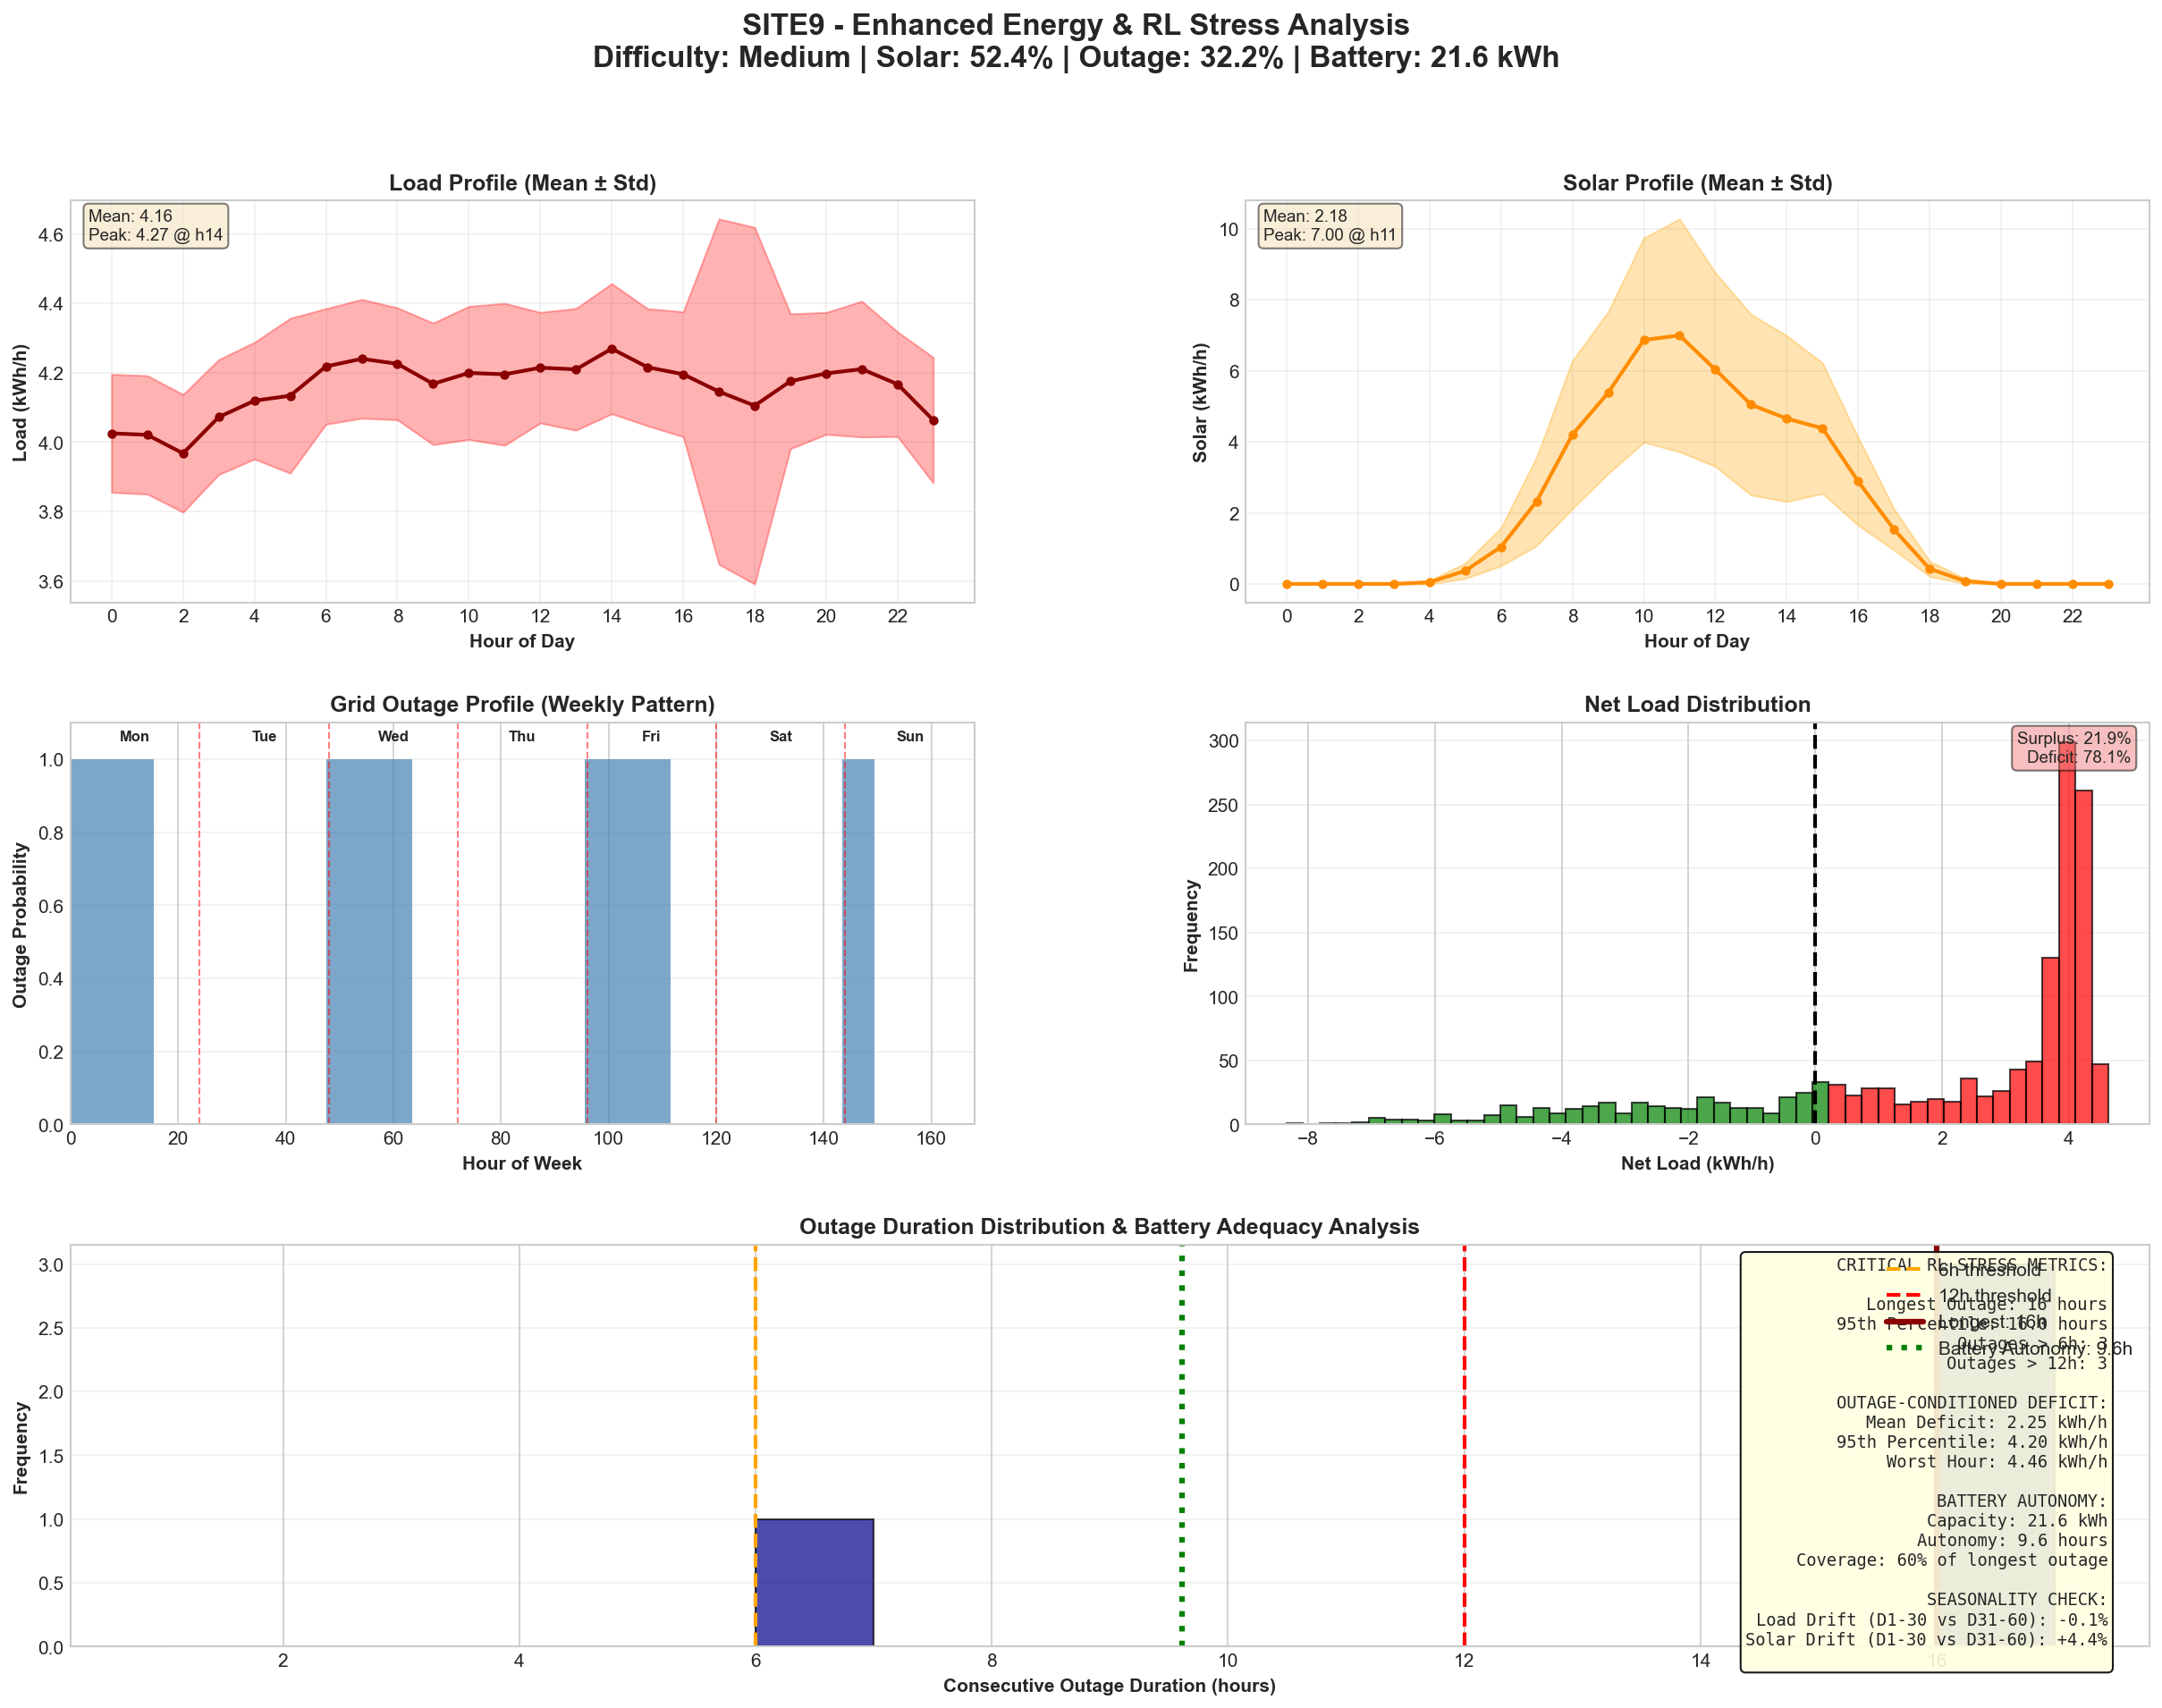
\includegraphics[width=\textwidth]{images/site9_enhanced_analysis}
\caption{Site~9 --- Medium. Load mean 4.16\,kWh/h; solar coverage 52.4\%;
battery autonomy 9.6\,h (60\% of longest outage). Three outages exceed
12\,h. Outage-conditioned mean deficit 2.25\,kWh/h. Moderate difficulty
across all dimensions.}
\label{fig:app_site9}
\end{figure}

\begin{figure}[htbp]
\centering
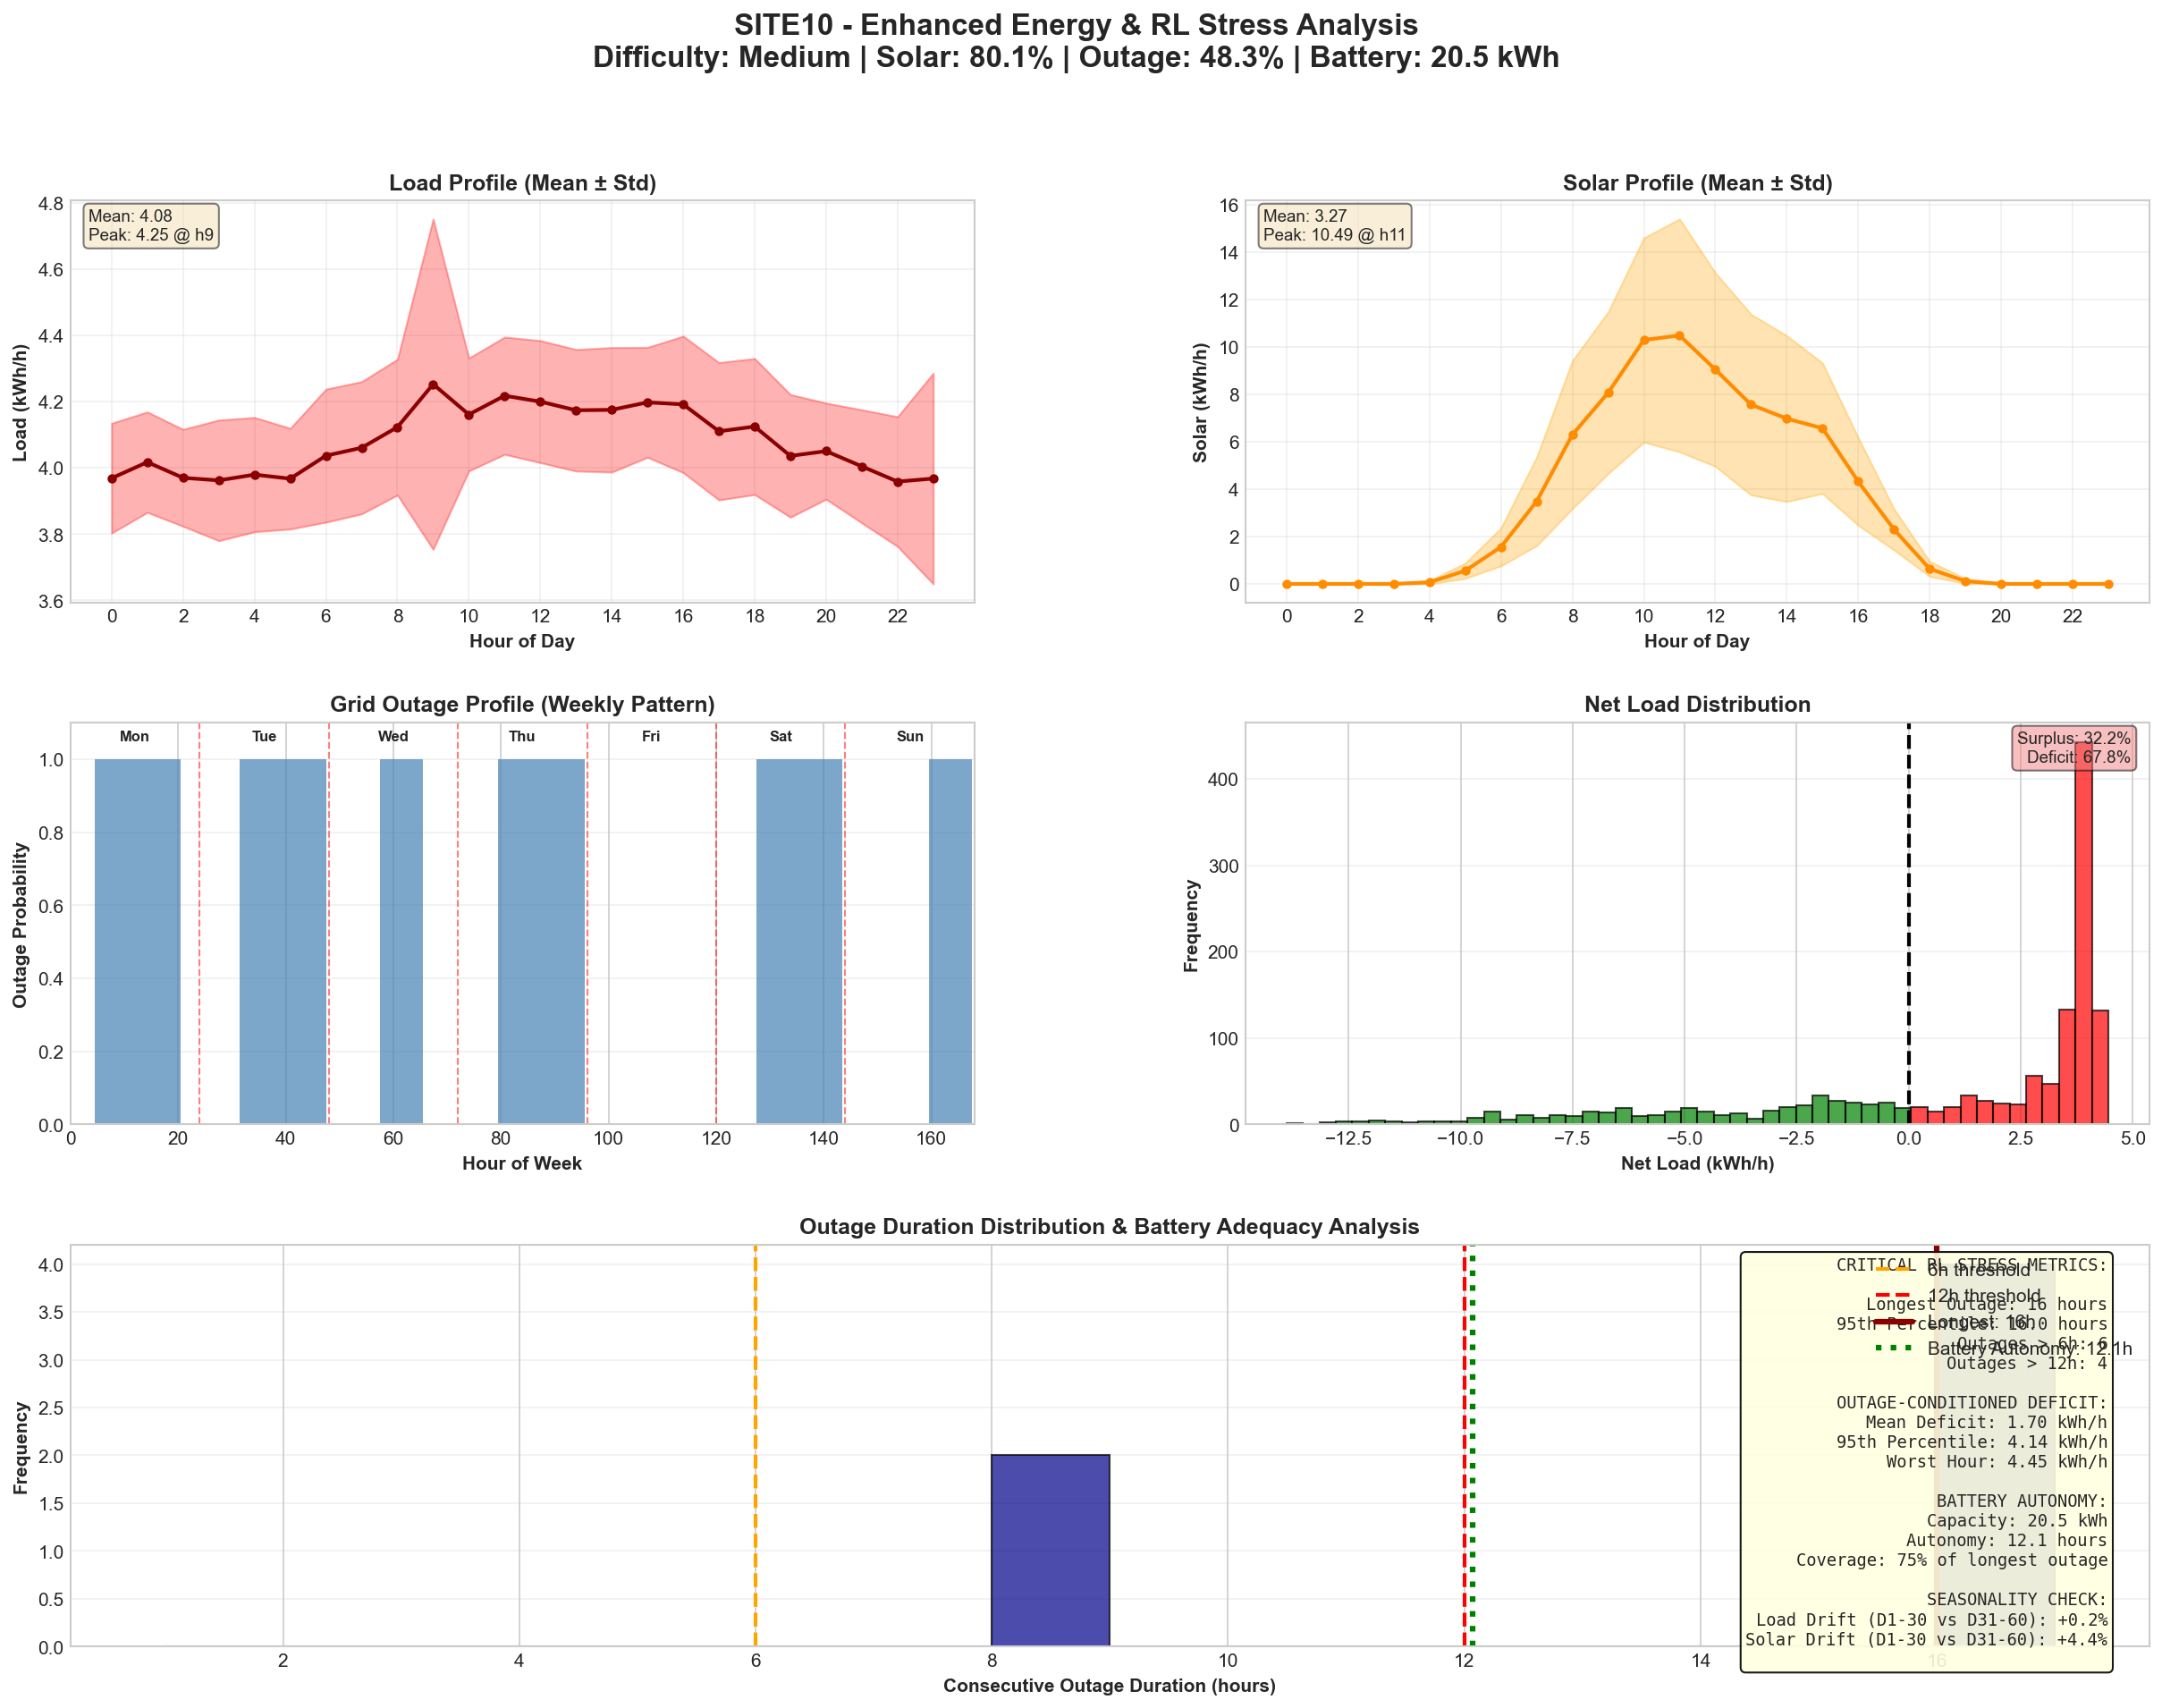
\includegraphics[width=\textwidth]{images/site10_enhanced_analysis}
\caption{Site~10 --- Medium (delayed-scenario edge case). Load mean
4.08\,kWh/h; solar coverage 80.1\%; battery autonomy 12.1\,h (75\% of
longest outage). Four outages exceed 12\,h. Despite a moderate composite score, high outage frequency (48.3\%)
combined with outages approaching battery autonomy makes this site
sensitive to logistics delays.}
\label{fig:app_site10}
\end{figure}

  \end{MainMatter}

  % ============== BACK MATTER (references etc.) ===================
  \begin{BackMatter}
    \printBibliographyReferences{references}
    % \printCV
    % \printCommittee
  \end{BackMatter}

\end{document}

